\section{Analysis}
\label{Analysis}
    \subsection{DataSet}
    \label{DataSet}
        The data used is a part of $pp$ collisions at $\sqrt{s}=13.6$ TeV obtained in 2022. The collision rate of $pp$ is $500$ kHz, and the dataset name is LHC22o$\_$apass7.
        The Monte Carlo simulation data used in \ref{Analysis:Matching} utilized Pythia8 Monash to reproduce 500 kHz $pp$ collisions at $\sqrt{s}=13.6$ TeV, employing minimum bias event simulations without extracting specific events.
        
    \subsection{Event selection}
    \label{Event_selection}
        The position of the proton-proton collision was measured by the ITS detector system. The Z-coordinate of the collision point, denoted as VtxZ, was selected with the condition $|VtxZ| < 10$ cm, using the ITS center at Z = 0 as the reference. This cut value is aligned with the ITS acceptance. The number of events obtained with this cut is $5.5 \times 10^9$.\@

    \subsection{Single muon track reconstruction}
    \label{Single_reco}
        As described in \ref{MFT-MUON_matching}, the reconstructed Global Track was used to calculate various physical quantities of the muon as follows: The muon's $\eta$ and $\phi$ were calculated using the MFT standalone Track. The momentum $p$ was derived by propagating the MCH standalone track to the Z-coordinate of the collision point, with corrections applied for multiple scattering and energy loss in the absorber.
        For the DCA, a Global Fit was performed for all tracks constituting the Global Track, and the resulting track was used. As shown in Fig. \ref{Analysis:reco:DCA}, the track was linearly extrapolated to the Z-coordinate of the collision point (IP), and the distance between the extrapolated point and the collision point was calculated as the DCA. Similarly, using the same track, $R_{abs}$ was calculated as the distance from the beam axis at the back edge of the absorber, as shown in Fig. \ref{Analysis:reco:R_abs}.\@
        Furthermore, the MFT-MCH matching $\chi^2$ was calculated based on the parameter differences when extrapolating the MFT track and MCH track to the matching plane.
        \begin{figure}[htbp]
            % Left figure
            \begin{minipage}{0.45\textwidth} % Specifying the width with minipage
                \centering
                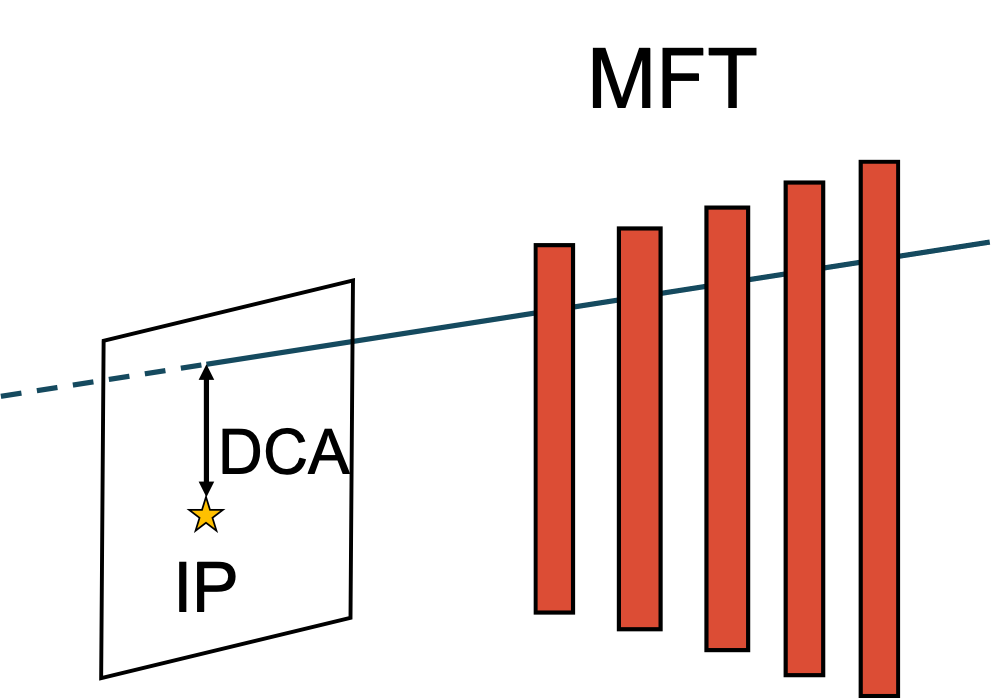
\includegraphics[keepaspectratio, scale=0.15]{fig/3_3_DCA.png} % Left image
                \caption{conceptual scheme of DCA}
                \label{Analysis:reco:DCA}
            \end{minipage}
            % Right figure
            \hspace{0.5cm}
            \begin{minipage}{0.45\textwidth}
                \centering
                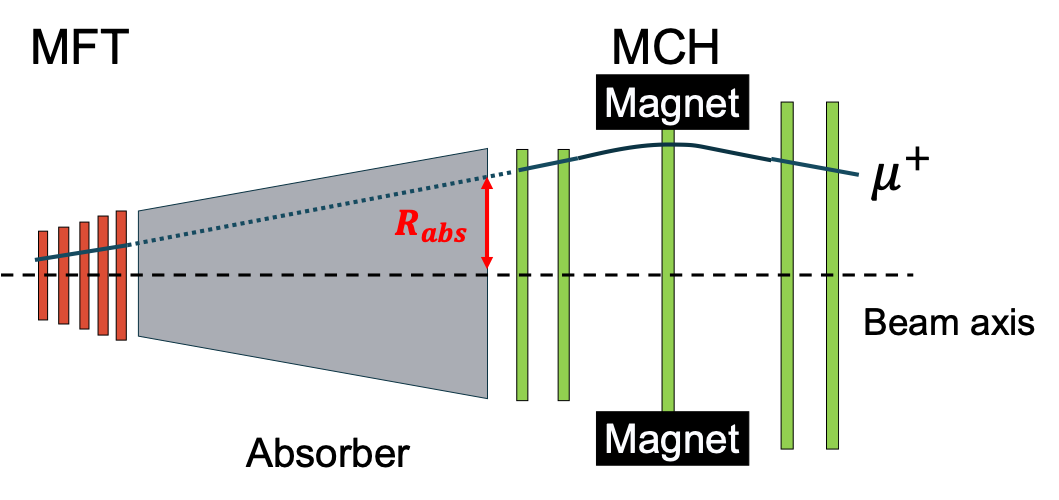
\includegraphics[keepaspectratio, scale=0.15]{fig/3_3_Rabs.png} % Right image
                \caption{conceptual scheme of $R_{abs}$}
                \label{Analysis:reco:R_abs}
            \end{minipage}
        \end{figure}

    \subsection{Single muon selection}
    \label{Single_muon_selection}
        The cuts applied to the obtained muon tracks are as follows:
        \begin{itemize}{}
            \item -3.6 <$\eta$ < -2.5
            \item 17.5 cm < $R_{abs}$ < 89.5 cm
            \item $pDCA$ < 6$\sigma$
            \item MFT-MCH matching $\chi^2$ < 30
        \end{itemize}
        The $\eta$ cut is aligned with the MFT-MHC-MID acceptance. The $R_{abs}$ cut value is set to exclude values that are influenced by the presence of the hadron absorber rear end. The $pDCA$ is the product of momentum and $DCA$, and this cut is applied to remove muons originating from beam gas. Tracks with $pDCA$ larger than 6$\sigma$ when fitted with a Gaussian distribution are excluded. 
        The final MFT-MCH matching $\chi^2$ value is obtained from a fit using the detected points of the MFT and MCH tracks when matching them. The value used in this study is optimized, as described later, to maximize the statistical uncertainty of the yields for $\omega$ and $\phi$. 
    
        \subsection{Dimuon analysis}
        \label{Dimuon}
            \subsubsection{Dimuon reconstruction}
            \label{Dimuon_reco}
                Using the single muons selected in \ref{Single_muon_selection}, dimuons are reconstructed. The mass($M_{\mu\mu}$), transverse momentum($p_T$), pseudorapidity($\eta$), and Azimuth angle($\phi$) of the dimuon are calculated as (\ref{px})~(\ref{eta_mumu}). First, the $p_T$, $\eta$, and $\phi$ of the single muons are converted into four-component vectors $(p_x, p_y, p_z, E)$ using (\ref{px}),(\ref{py}),(\ref{pz}),(\ref{E}).\@
                \begin{eqnarray}
                    p_x &=& p_T \cos(\phi)\\ \label{px}
                    p_y &=& p_T \sin (\phi)\\ \label{py}
                    p_z &=& p_T \sinh (\eta)\\ \label{pz}
                    E &=& \sqrt{p_T^2 \cosh^2(\eta) + m_\mu^2} \label{E} 
                \end{eqnarray}
                Then, using the $(p_x, p_y, p_z, E)$ of the single muons, the $(P_x, P_y, P_z, E_{\mu\mu})$ of the dimuon are calculated.
                \begin{eqnarray}
                    \begin{pmatrix}
                        P_x \\
                        P_y \\
                        P_z \\
                        E
                    \end{pmatrix}
                    &=&
                    \begin{pmatrix}
                        p_{x1} \\
                        p_{y1} \\
                        p_{z1} \\
                        E_1
                    \end{pmatrix}
                    +
                    \begin{pmatrix}
                        p_{x2} \\
                        p_{y2} \\
                        p_{z2} \\
                        E_2
                    \end{pmatrix}
                \end{eqnarray}
                Using the obtained four-component vector of the dimuon $(Px, Py, Pz, E_{\mu\mu})$, the pair's $M_\mu\mu$, $p_T$, and $\eta$ were calculated from the (\ref{M_mumu}),(\ref{pT_mumu}),(\ref{eta_mumu}).
                \begin{eqnarray}
                    M_{\mu\mu} &=& \sqrt{E^2 - (p_x^2 + p_y^2 + p_z^2)}\\ \label{M_mumu}
                    p_{T\mu\mu} &=& \sqrt{p_x^2 + p_y^2}\\ \label{pT_mumu}
                    \eta_{\mu\mu} &=& -\log\left(\tan\left(\frac{1}{2}\arctan\left(\frac{\sqrt{p_x^2 + p_y^2}}{p_z}\right)\right)\right) \label{eta_mumu}
                \end{eqnarray}
                Using the above formulas, the physical quantities of the dimuon are calculated.
                
            \subsubsection{Combinatorial background subtraction}
            \label{Analysis:Dimuon:Combinatorial BG subtraction}
                The dimuon was reconstructed by pairing oppositely charged muons present in each event.In cases where there are multiple combinations, all combinations are used to pair the muons and reconstruct the physical quantities of the dimuon. Since all combinations are considered, the mass distribution of uncorrelated muon pairs is also reconstructed. This is called the combinatorial background. In this study, the Like Sign method is used to subtract the combinatorial background. The Like Sign method is a method that estimates the combinatorial background by using the mass distribution of muon pairs with the same sign from each collision event. The key feature of this method is that it estimates the shape of uncorrelated background events using the like-sign muons from the same event, allowing for the subtraction of mass distributions of weakly correlated particles within each event, such as those arising from elliptic flow in heavy-ion collisions. The estimated uncorrelated background events depend on the $p_T$ of the dimuon.
                The calculation formula is given by (\ref{LikeSignMethod}).
                \begin{eqnarray}
                    \label{LikeSignMethod}
                    \dv{N_{sig}}{m} &=& \dv{N_{same}^{+-}}{m} - 2R \sqrt{\dv{N_{same}^{++}}{m} \dv{N_{same}^{--}}{m}}\\
                    2R &=& \frac{\dv{N_{mix}^{+-}}{m}}{\sqrt{\dv{N_{mix}^{++}}{m} \dv{N_{mix}^{--}}{m}}} 
                \end{eqnarray}
                where, $\dv{N_{sig}}{m}$ represents the number of correlated muons at each mass, $\dv{N_{same}^{**}}{m}$ represents the number of same-sign muon pairs in the same event (** corresponds to the muon sign), and $\dv{N_{mix}^{**}}{m}$ represents the number of muon pairs formed from different events. R is a term to correct for the acceptance difference due to the muon sign. If there is no acceptance difference due to the sign, R = 1. In this analysis, since muon pairs from different events were not reconstructed, R = 1 was used for the calculation.

                The result of the combinatorial background subtraction in the dimuon transverse momentum region of (1 < $p_T$ < 30) GeV is shown Fig.\ref{All_pt_CB}.
                \begin{figure}[H]
                    \centering
                    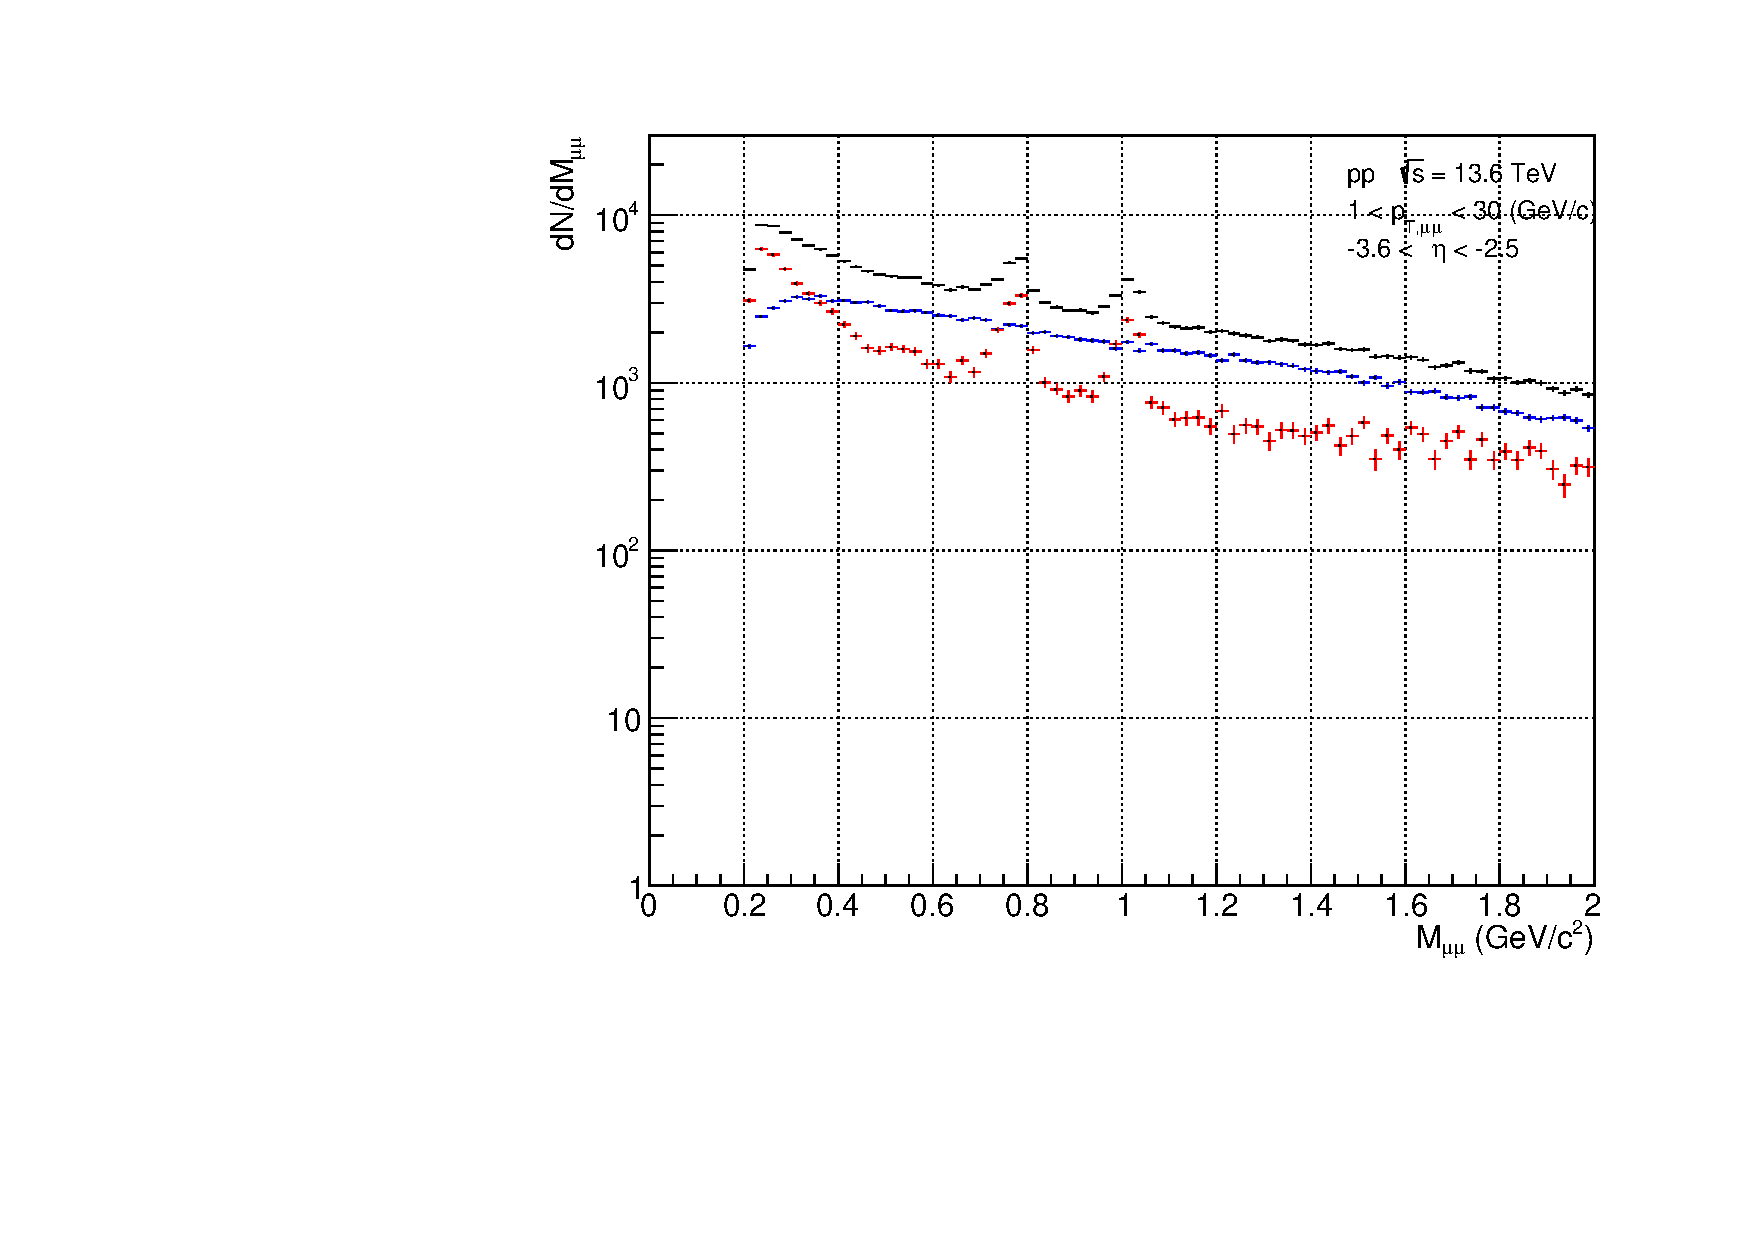
\includegraphics[keepaspectratio, scale=0.5]{fig/3_4_1_CB_pt_1to30.pdf}
                    \caption{1 < $p_{T}$ < 30}
                    \label{All_pt_CB}
                \end{figure}
                The black distribution represents the invariant mass reconstructed by pairing oppositely charged muon particles from all combinations within the same event, while the blue distribution represents the uncorrelated background events estimated using the Like Sign method. The red distribution, obtained by subtracting the blue from the black one, represents the dimuon invariant mass distribution with correlations.
                To examine the transverse momentum dependence of the $\omega$ and $\phi$ yields, the mass distributions were separated by dimuon $p_T$, and uncorrelated background events were subtracted using the Like Sign method in each invariant mass distribution. The subtracted plots are shown in Fig.\ref{Analysis:Dimuon:CB:CB_pt_separation}.

                \begin{figure}[H]
                    \centering
                    \begin{minipage}{0.45\textwidth}
                        \centering
                        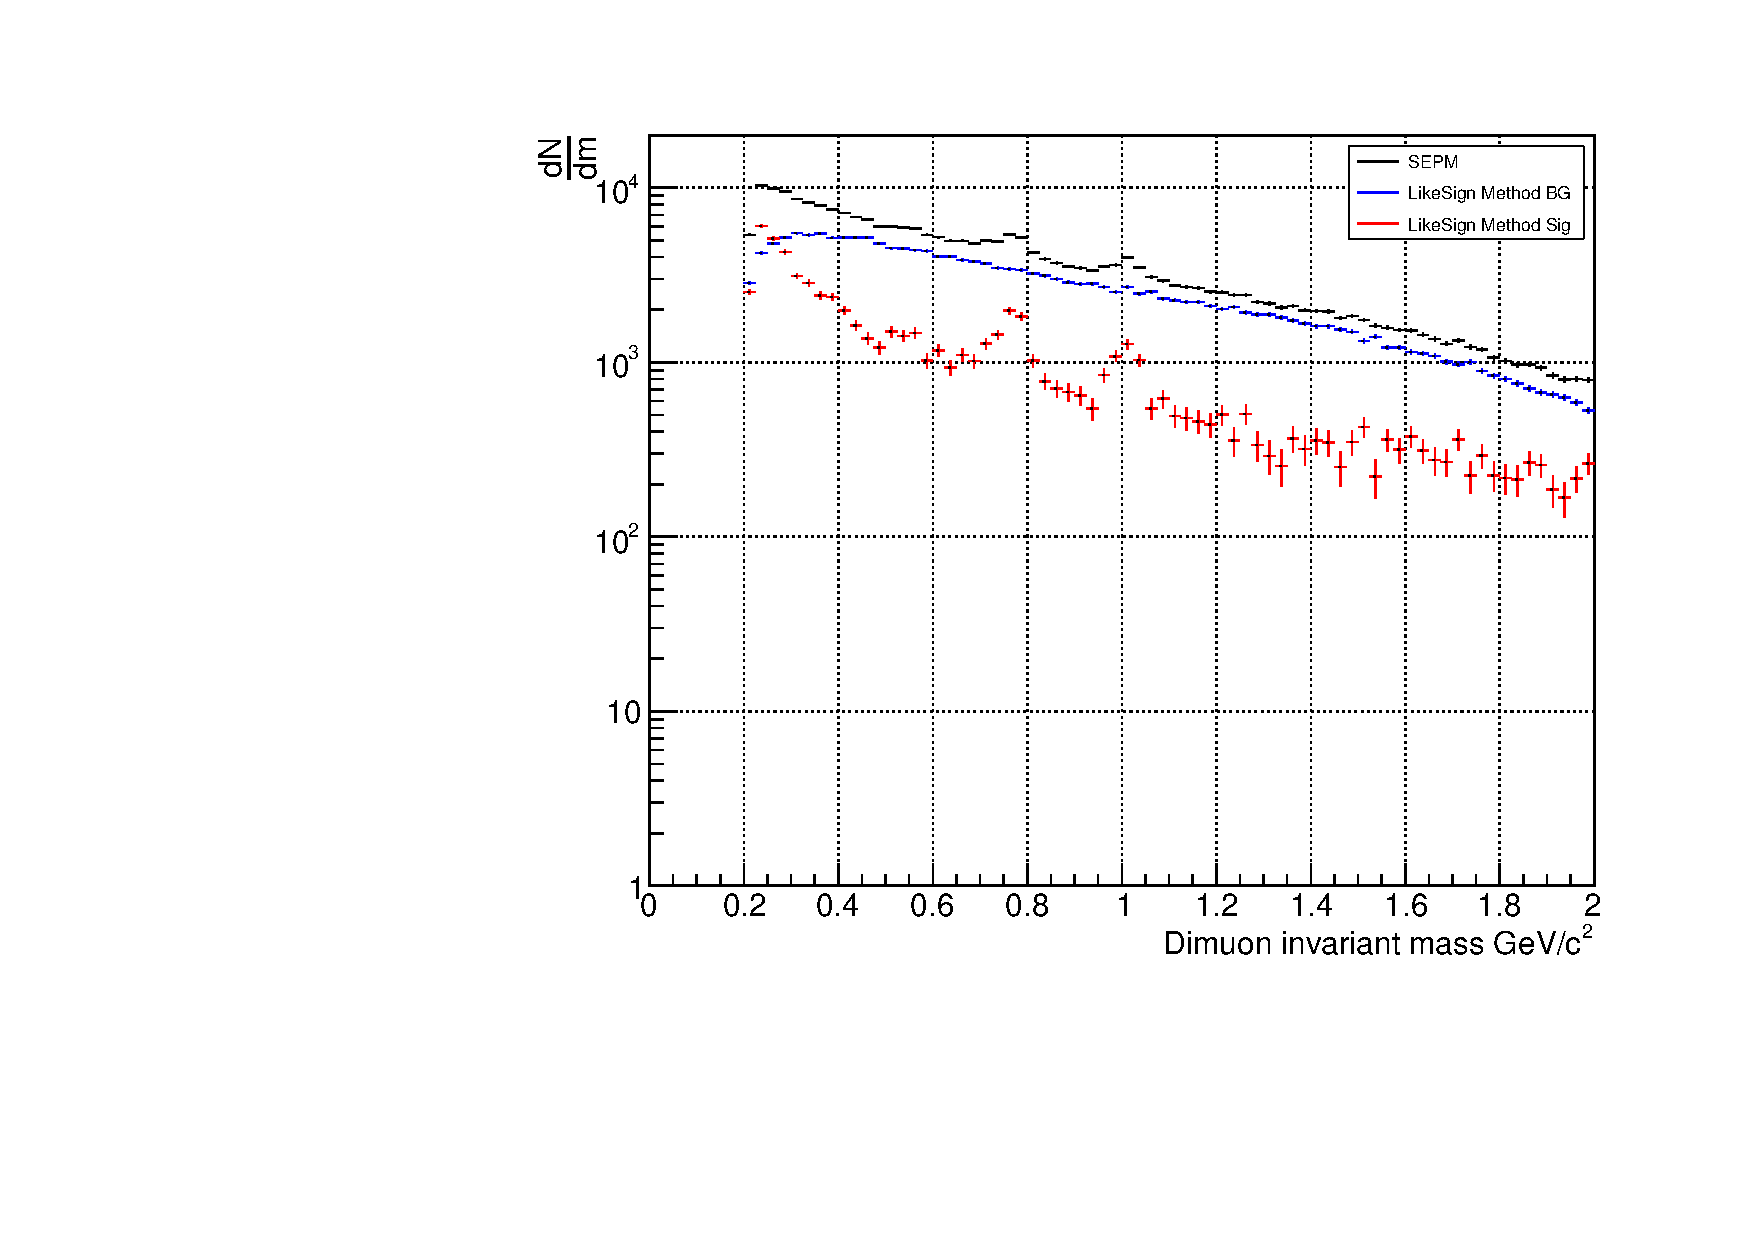
\includegraphics[width=\textwidth]{fig/3_4_1_CB_pt_1to2.pdf}
                        \caption*{1 < $p_{T}$ < 2}
                    \end{minipage}
                    \hfill
                    \begin{minipage}{0.45\textwidth}
                        \centering
                        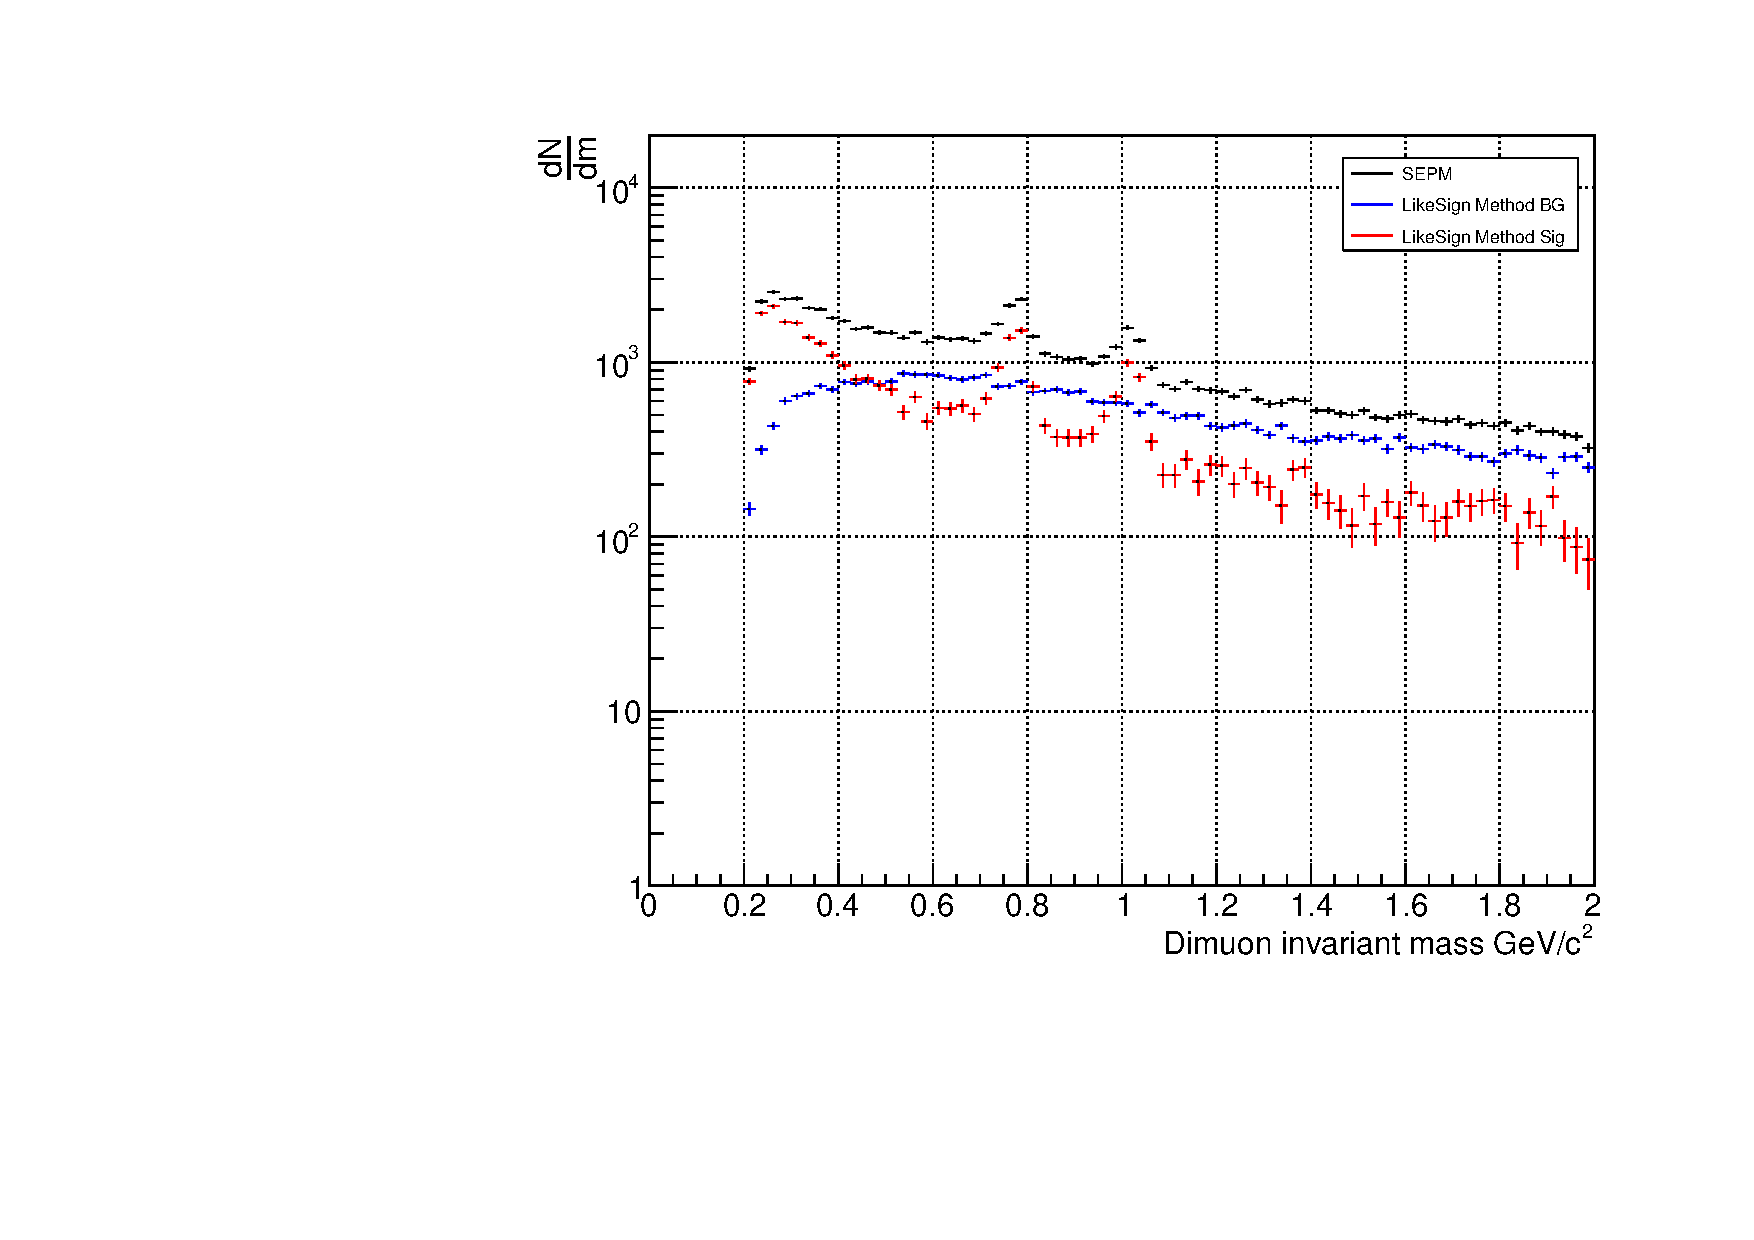
\includegraphics[width=\textwidth]{fig/3_4_1_CB_pt_2to3.pdf}
                        \caption*{2 < $p_{T}$ < 3}
                    \end{minipage}
                    \\
                    \vspace{1em}
                    \begin{minipage}{0.45\textwidth}
                        \centering
                        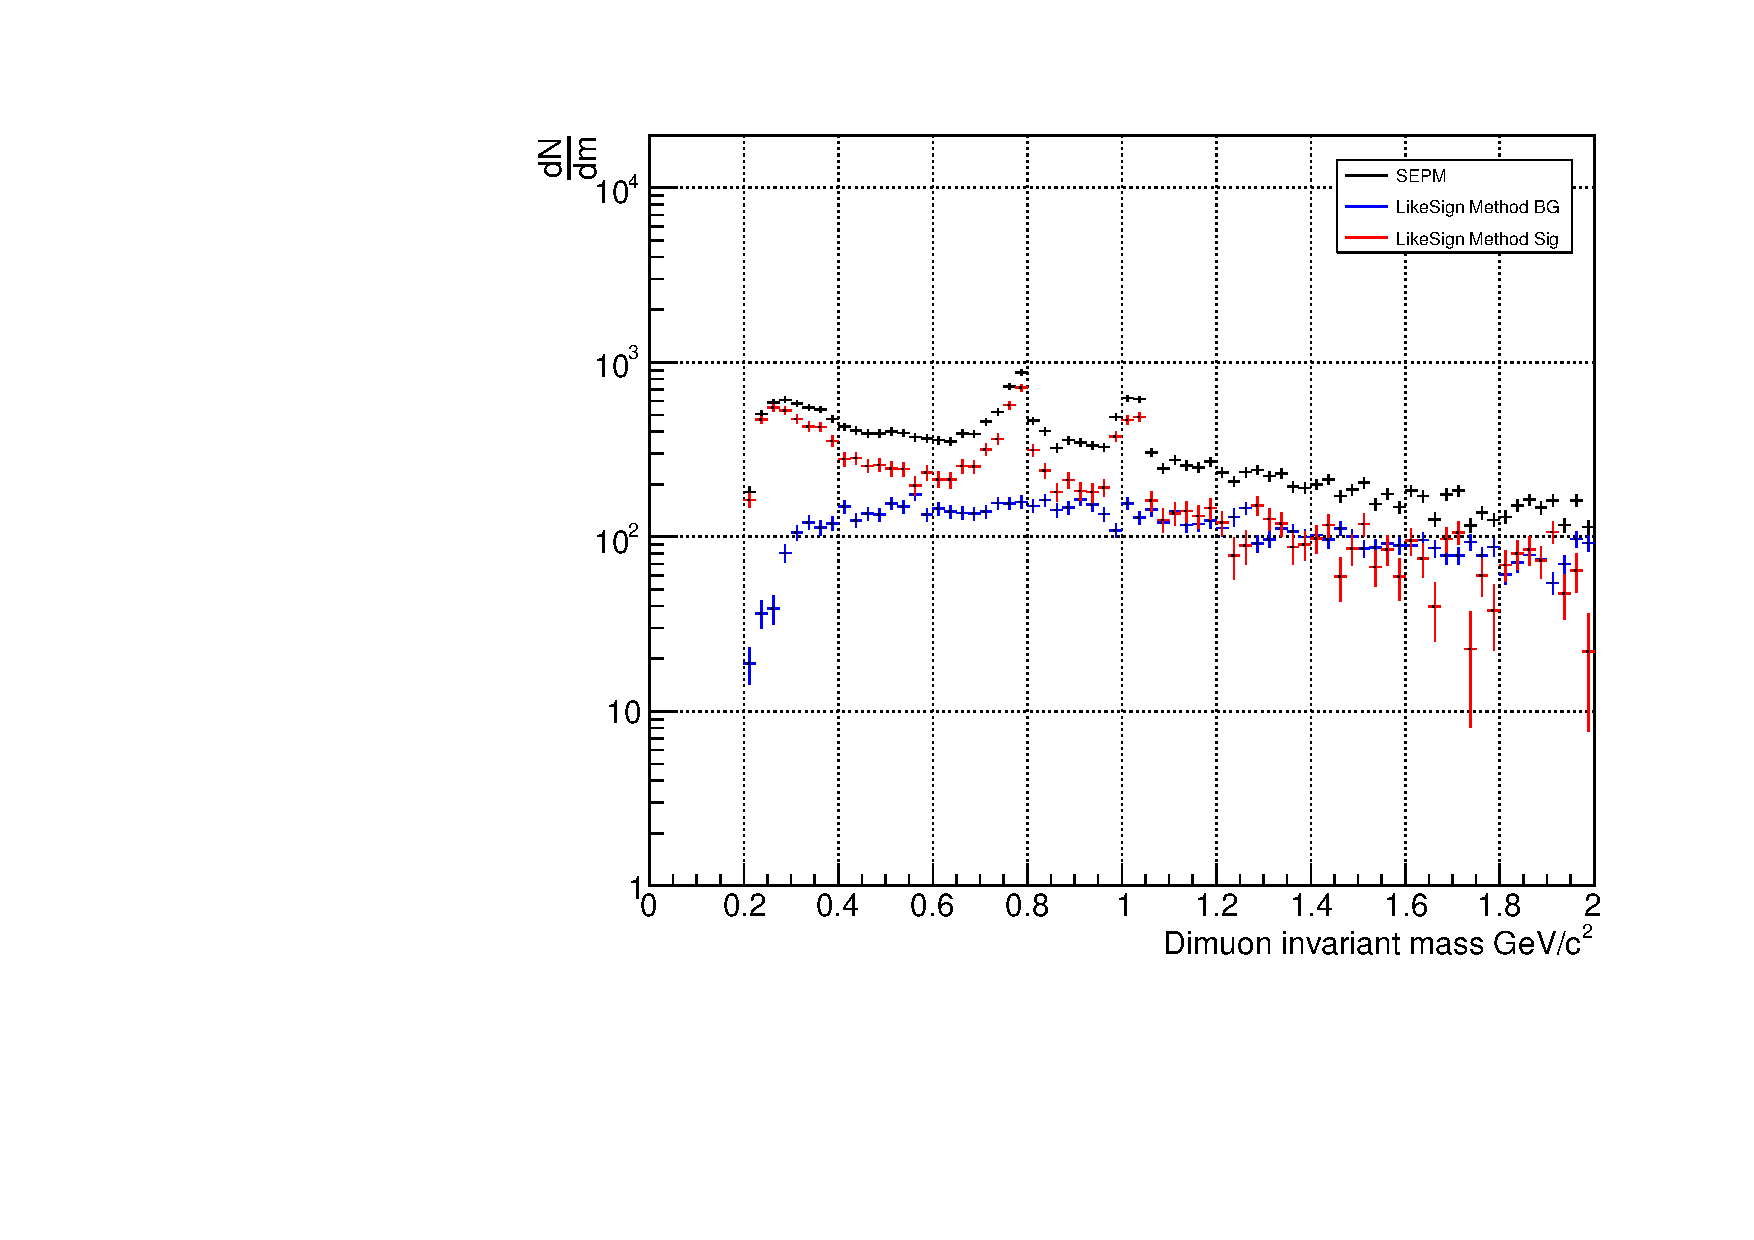
\includegraphics[width=\textwidth]{fig/3_4_1_CB_pt_3to4.pdf}
                        \caption*{3 < $p_{T}$ < 4}
                    \end{minipage}
                    \hfill
                    \begin{minipage}{0.45\textwidth}
                        \centering
                        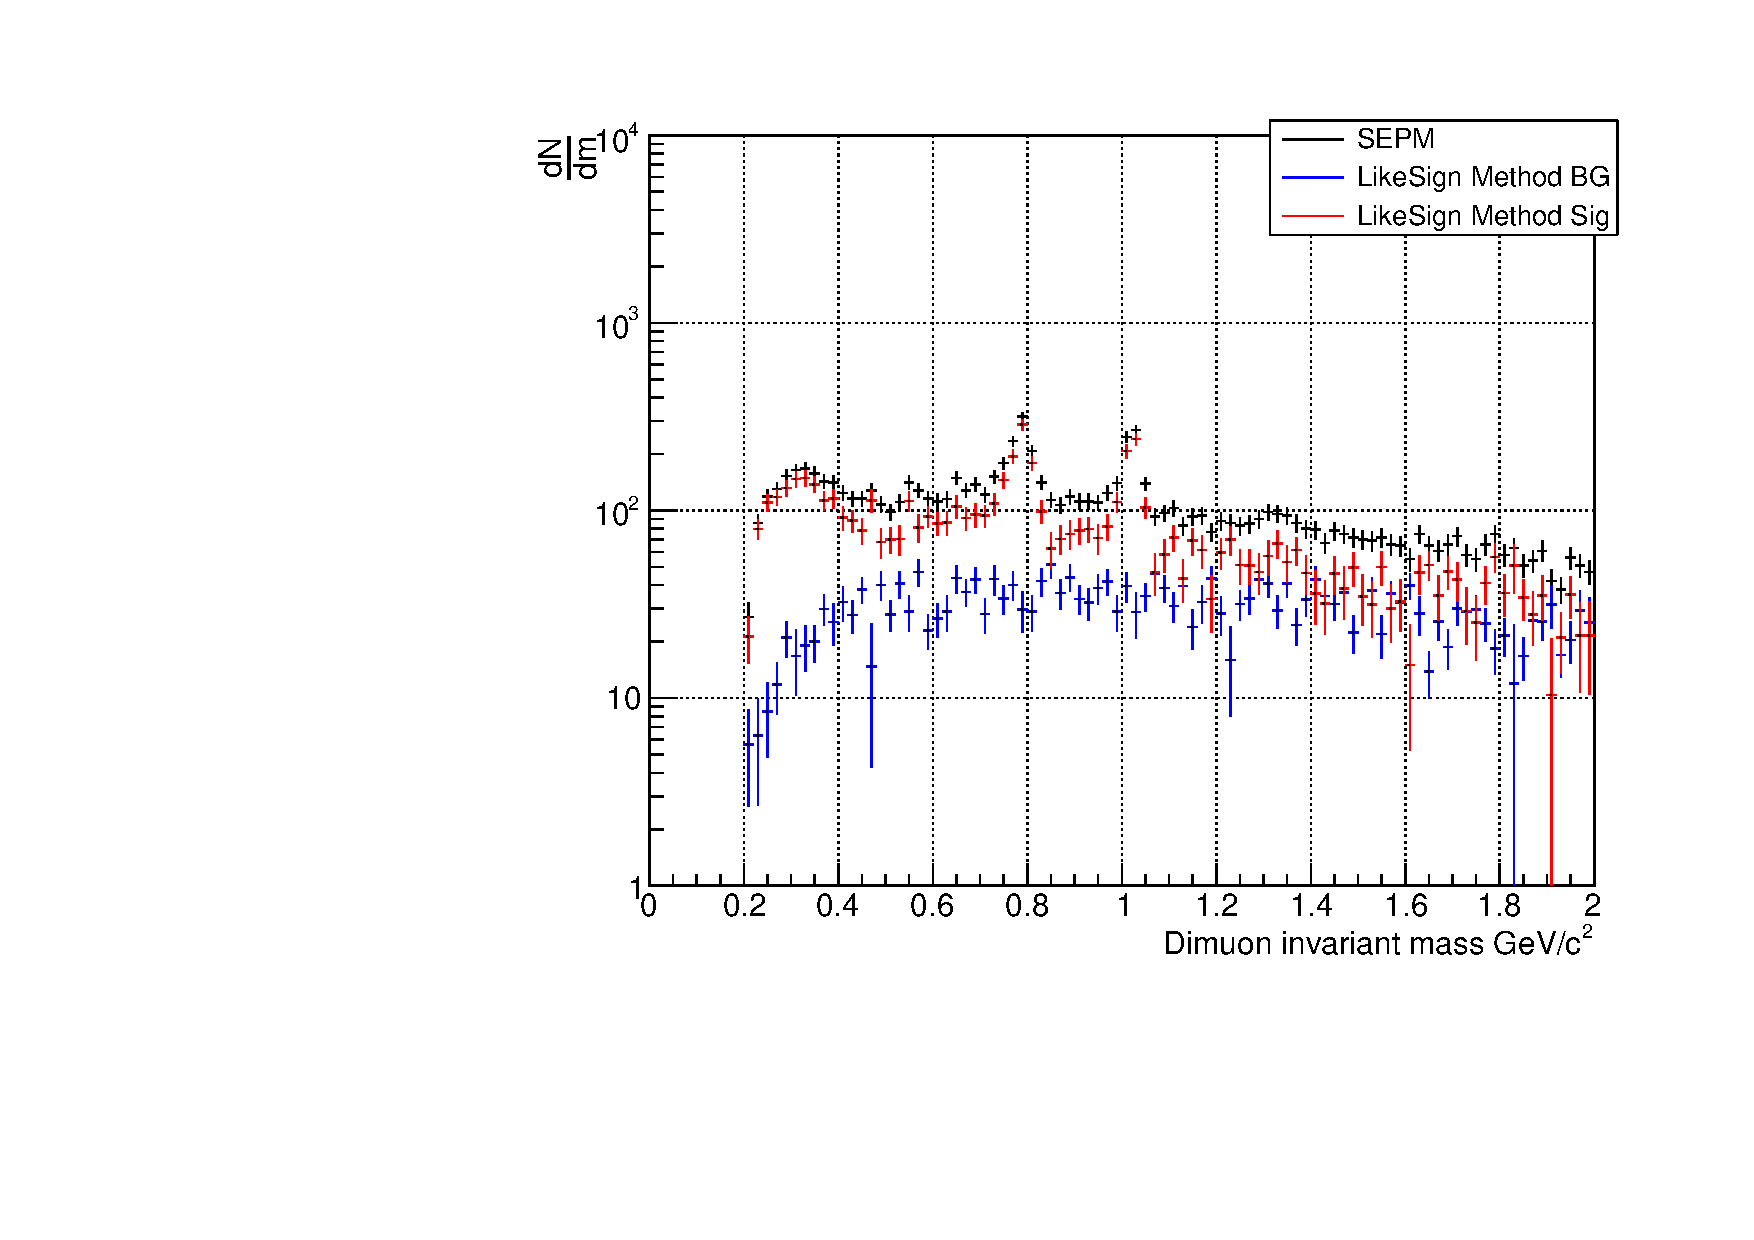
\includegraphics[width=\textwidth]{fig/3_4_1_CB_pt_4to5.pdf}
                        \caption*{4 < $p_{T}$ < 5}
                    \end{minipage}
                    \\
                    \vspace{1em}
                    \begin{minipage}{0.45\textwidth}
                        \centering
                        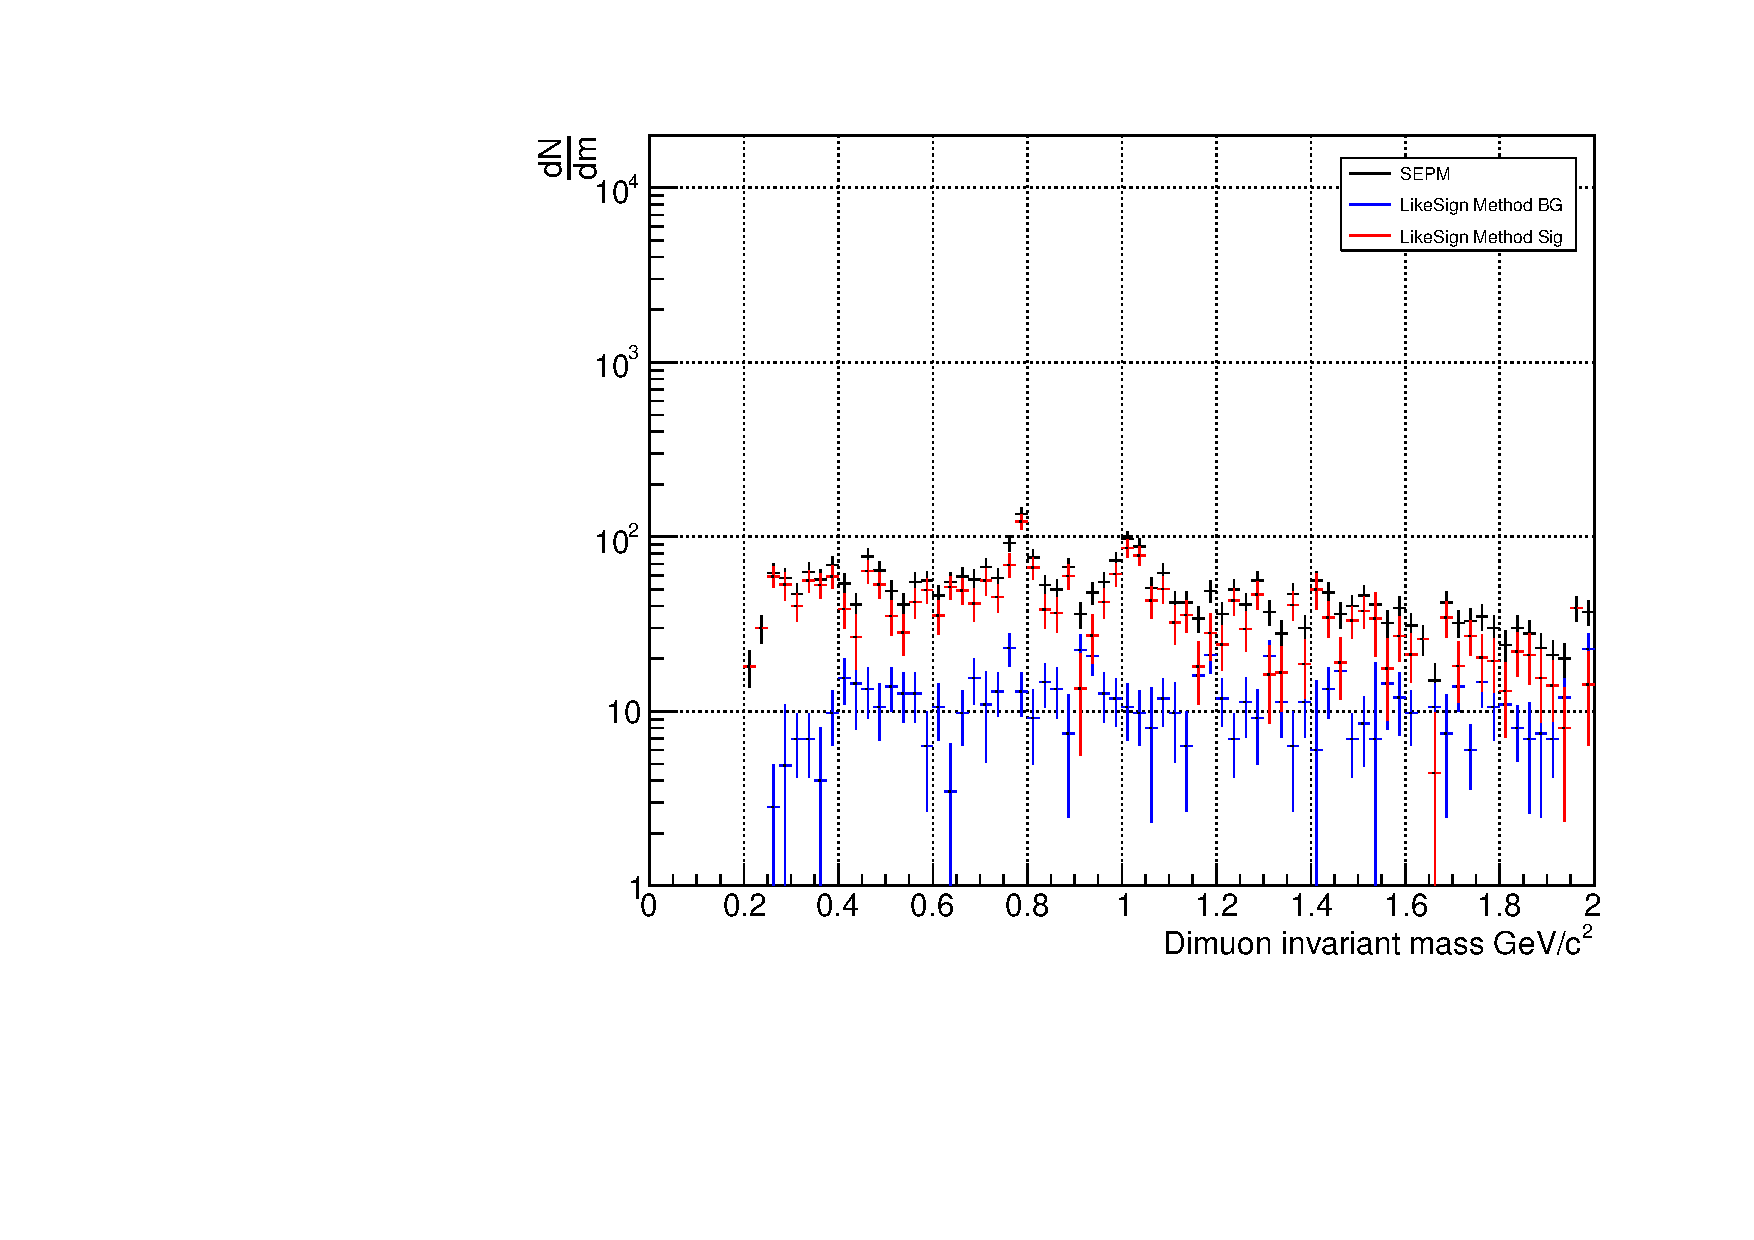
\includegraphics[width=\textwidth]{fig/3_4_1_CB_pt_5to6.pdf}
                        \caption*{5 < $p_{T}$ < 6}
                    \end{minipage}
                    \hfill
                    \begin{minipage}{0.45\textwidth}
                        \centering
                        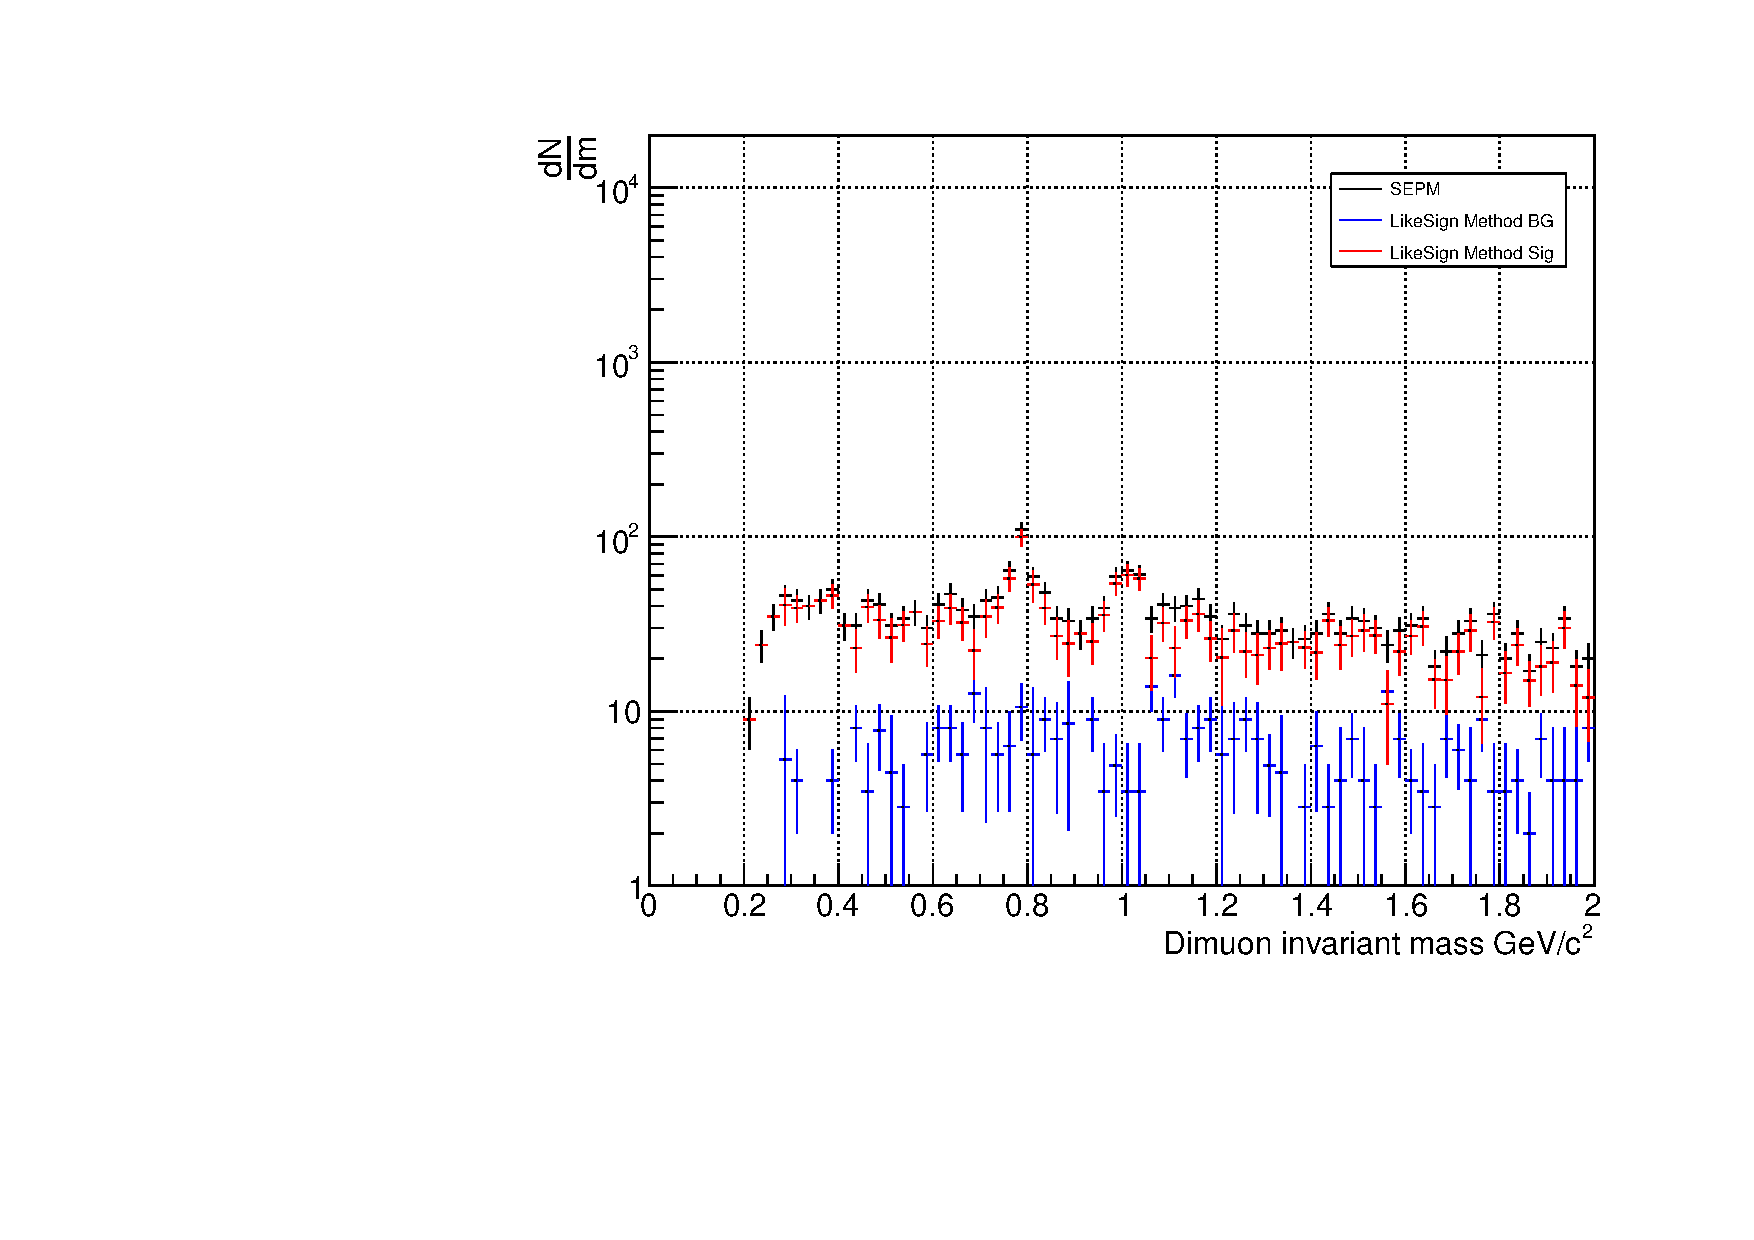
\includegraphics[width=\textwidth]{fig/3_4_1_CB_pt_6to10.pdf}
                        \caption*{6 < $p_{T}$ < 10}
                    \end{minipage}
                    \caption{Result of combinatorial background subtracktion of each $p_T$}
                    \label{Analysis:Dimuon:CB:CB_pt_separation}
                \end{figure}
                In the region of \(0 < p_T < 1\) GeV, no peaks for \(\omega\) and \(\phi\) were observed. This is believed to be due to insufficient resolution of the single muon \(p_T\) and the dominance of tracks with incorrect MFT-MCH matching. The region of \(6 < p_T < 10\) GeV was chosen to be wider than other transverse momentum regions in order to preserve the statistical significance.
        
            \subsubsection{Peak extraction of $\omega \rightarrow \mu\mu ,\phi \rightarrow \mu\mu$}
            \label{Peak_extraction}
                The distributions of the correlated dimuon invariant mass obtained from \ref{Analysis:Dimuon:Combinatorial BG subtraction} are used to extract the distributions of $\omega \rightarrow \mu\mu,\phi \rightarrow \mu\mu$. The dimuon invariant mass distribution under 2($GeV/c^2$) contains pairs of muons coming from light flavor mesons and open heavy flavor. Charm and bottom quarks have heavy masses and are produced through pair creation in the initial collision. The pair-created \(c\bar{c}\) quarks separate and form \(D\bar{D}\) mesons. The \(D\) and \(\bar{D}\) mesons undergo semileptonic decays, such as \(D \rightarrow \bar{K}^0 + \mu^+ + \nu_\mu\) or \(D \rightarrow \mu^+ + \nu_\mu\), and \(\bar{D} \rightarrow K^0 + \mu^- + \nu_\mu\) or \(\bar{D} \rightarrow \mu^- + \nu_\mu\). Since the parent \(D\) and \(\bar{D}\) mesons are produced through pair creation, they are strongly correlated, and their decay products, the muons, also exhibit correlation. As a result, the dimuon mass distribution with correlations is included. The same correlation applies in the case of \(B\) mesons.
                \begin{itemize}
                    \item $\eta \rightarrow \mu^+ \mu^-$
                    \item $\eta \rightarrow \mu^+ \mu^- \gamma$
                    \item $\rho \rightarrow \mu^+ \mu^-$
                    \item $\omega \rightarrow \mu^+ \mu^-$
                    \item $\omega \rightarrow \mu^+ \mu^- \pi^0$
                    \item $\eta' \rightarrow \mu^+ \mu^- \gamma$
                    \item $\phi \rightarrow \mu^+ \mu^-$
                    \item $c\bar{c} \rightarrow D\bar{D} \rightarrow \mu^+ \mu^- + others$
                    \item $b\bar{b} \rightarrow B\bar{B} \rightarrow \mu^+ \mu^- + others$
                \end{itemize}
                The decays \(\omega \rightarrow \mu\mu\) and \(\phi \rightarrow \mu\mu\) are known to exhibit sharp peak structures from previous lepton pair measurements, forming peaks near 0.8 \(\mathrm{GeV/c^2}\) and 1.0 \(\mathrm{GeV/c^2}\) in the mass distribution.
                It is known that no sharp peak structures exist for any decays other than the two-body decays of \(\omega\) and \(\phi\). Therefore, the continuous component was fitted using an exponential function. The fitting was performed in the range of 0.5 < \(M_{\mu\mu}\) < 1.3 \(\mathrm{GeV/c^2}\), excluding the regions with peak structures at 0.7 < \(M_{\mu\mu}\) < 0.86 and 0.92 < \(M_{\mu\mu}\) < 1.15. The continuous component was fitted using the exponential function shown (\ref{fit:BG}).
                \begin{eqnarray}
                    \label{fit:BG}
                    f_{BG}(m)=N_0*\exp{-p1* m}
                \end{eqnarray}
                where, \(N_0\) and \(p1\) are the fit parameters. The continuous component mass distribution was subtracted using the results from the fit, and Gaussian fits were performed for the \(\omega\) and \(\phi\) in the mass regions 0.7 < \(M_{\mu\mu}\) < 0.86 \(\mathrm{GeV/c^2}\) and 0.92 < \(M_{\mu\mu}\) < 1.15 \(\mathrm{GeV/c^2}\), respectively. The fitting function is given by (\ref{fit:omega}) and (\ref{fit:phi}).
                \begin{eqnarray}
                    \label{fit:omega}
                    f_{\omega} &=& N_{\omega}*\exp{-\frac{1}{2}\qty(\frac{m-M_{\omega}}{\sigma_{\omega}})^2}\\\
                    \label{fit:phi}
                    f_{\phi} &=& N_{\phi}*\exp{-\frac{1}{2}\qty(\frac{m-M_{\phi}}{\sigma_{\phi}})^2}
                \end{eqnarray}
                The fit parameters are \(N_{\omega}, N_{\phi}, M_{\omega}, M_{\phi}, \sigma_{\omega}, \sigma_{\phi}\). Specifically, \(M_{\omega}\) and \(M_{\phi}\) correspond to the mean mass positions of \(\omega\) and \(\phi\), while \(\sigma_{\omega}\) and \(\sigma_{\phi}\) correspond to the mass widths. Using the fit parameters obtained from the continuous component and the Gaussian fits for \(\omega\) and \(\phi\), all functions were combined, and a global fit was performed to extract the mean mass positions and mass widths of \(\omega\) and \(\phi\). The fit range is 0.5 < \(M_{\mu\mu}\) < 1.3 \(\mathrm{GeV/c^2}\). The function for the overall fit is given by the (\ref{fit:globalfit}).
                \begin{eqnarray}
                    \label{fit:globalfit}
                    f(m)=N_0*\exp{-p1* m}+N_{\omega}*\exp{-\frac{1}{2}\qty(\frac{m-M_{\omega}}{\sigma_{\omega}})^2}+N_{\phi}*\exp{-\frac{1}{2}\qty(\frac{m-M_{\phi}}{\sigma_{\phi}})^2}
                \end{eqnarray}
                The parameters for the overall fit are similarly \(N_0, N_{\omega}, N_{\phi}, M_{\omega}, M_{\phi}, \sigma_{\omega}, \sigma_{\phi}\). The fit results are shown in Figure \ref{Analysis:Dimuon:Yield:fit} and Table \ref{Analysis:Dimuon:Yield:Fit_Results}.
                \begin{figure}[H]
                    \centering
                    \begin{minipage}{0.45\textwidth}
                        \centering
                        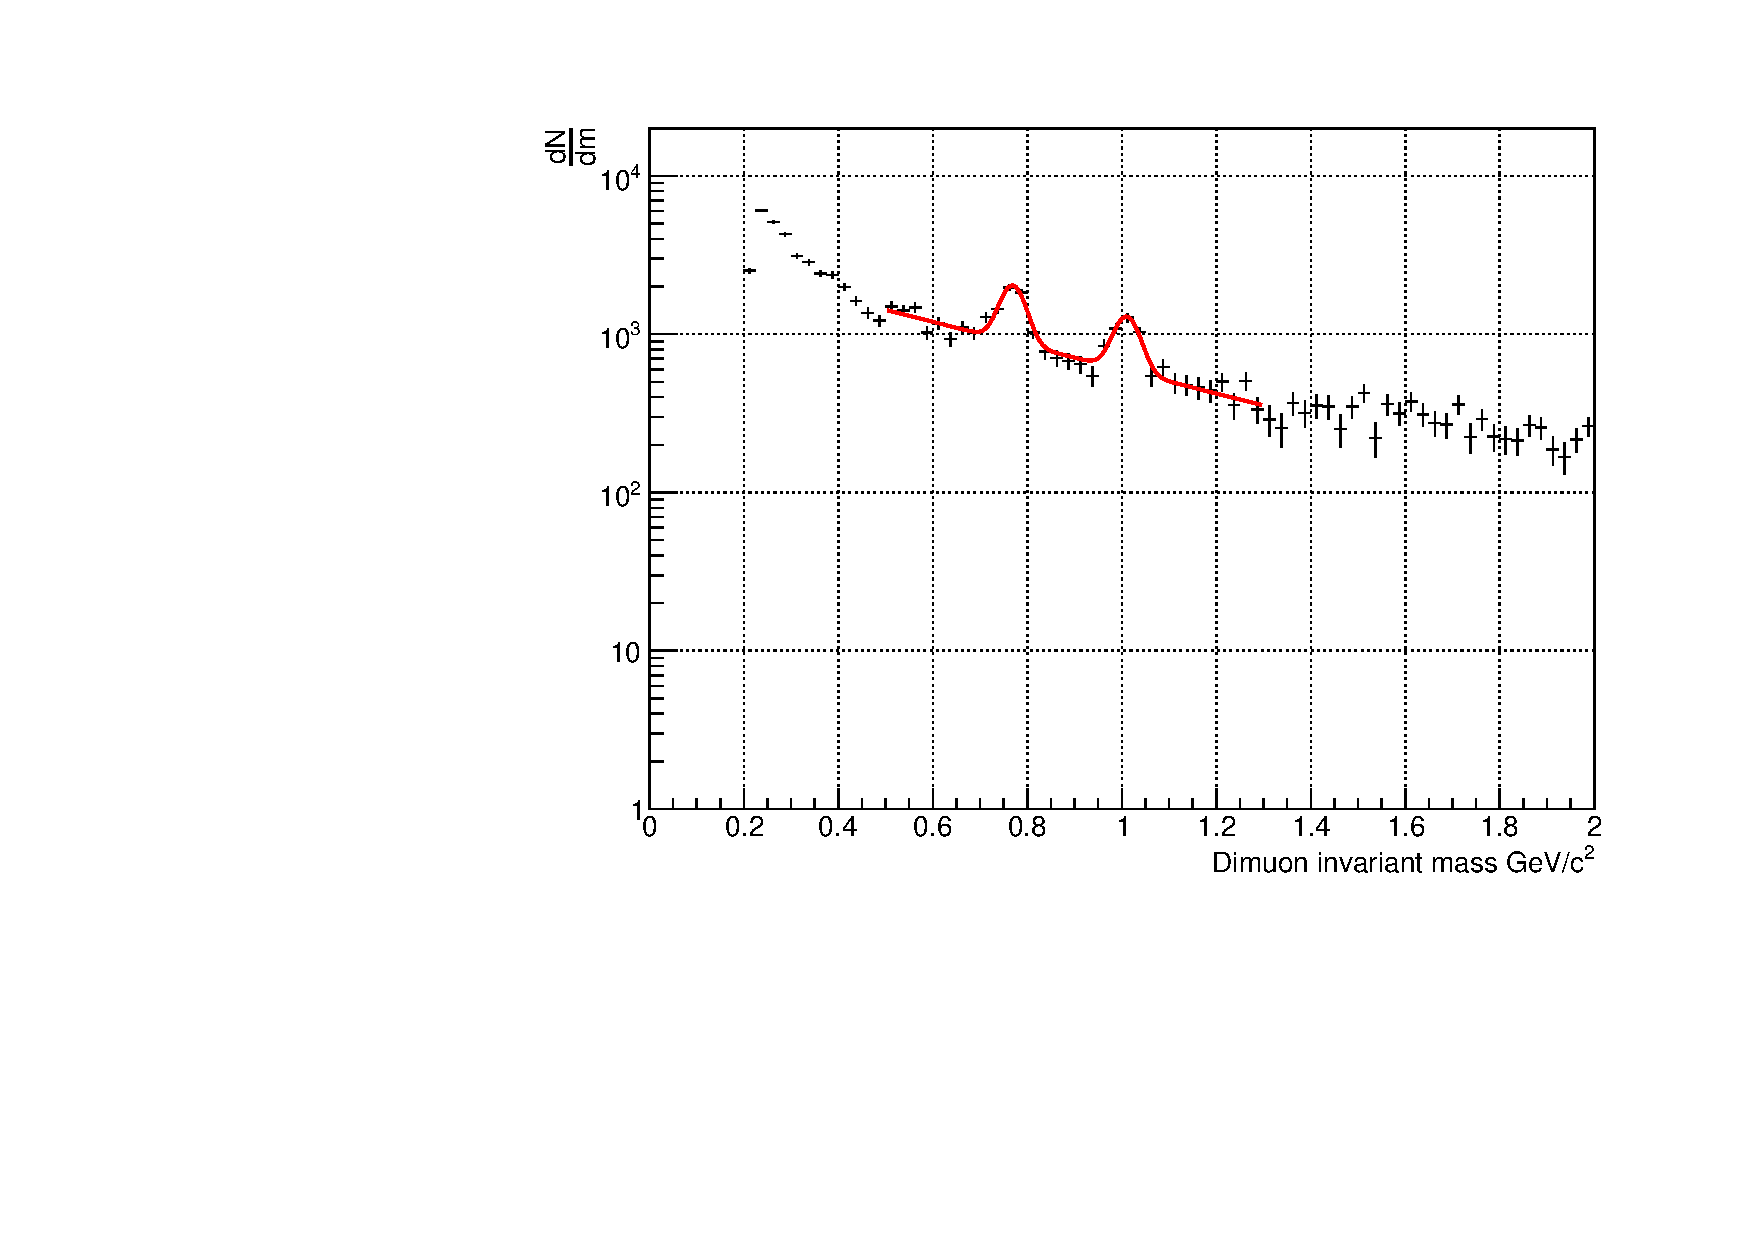
\includegraphics[width=\textwidth]{fig/3_4_2_fit_pt_1to2.pdf}
                        \captionsetup{labelformat=empty}
                        \caption*{1 < $p_{T}$ < 2}
                    \end{minipage}
                    \hfill
                    \begin{minipage}{0.45\textwidth}
                        \centering
                        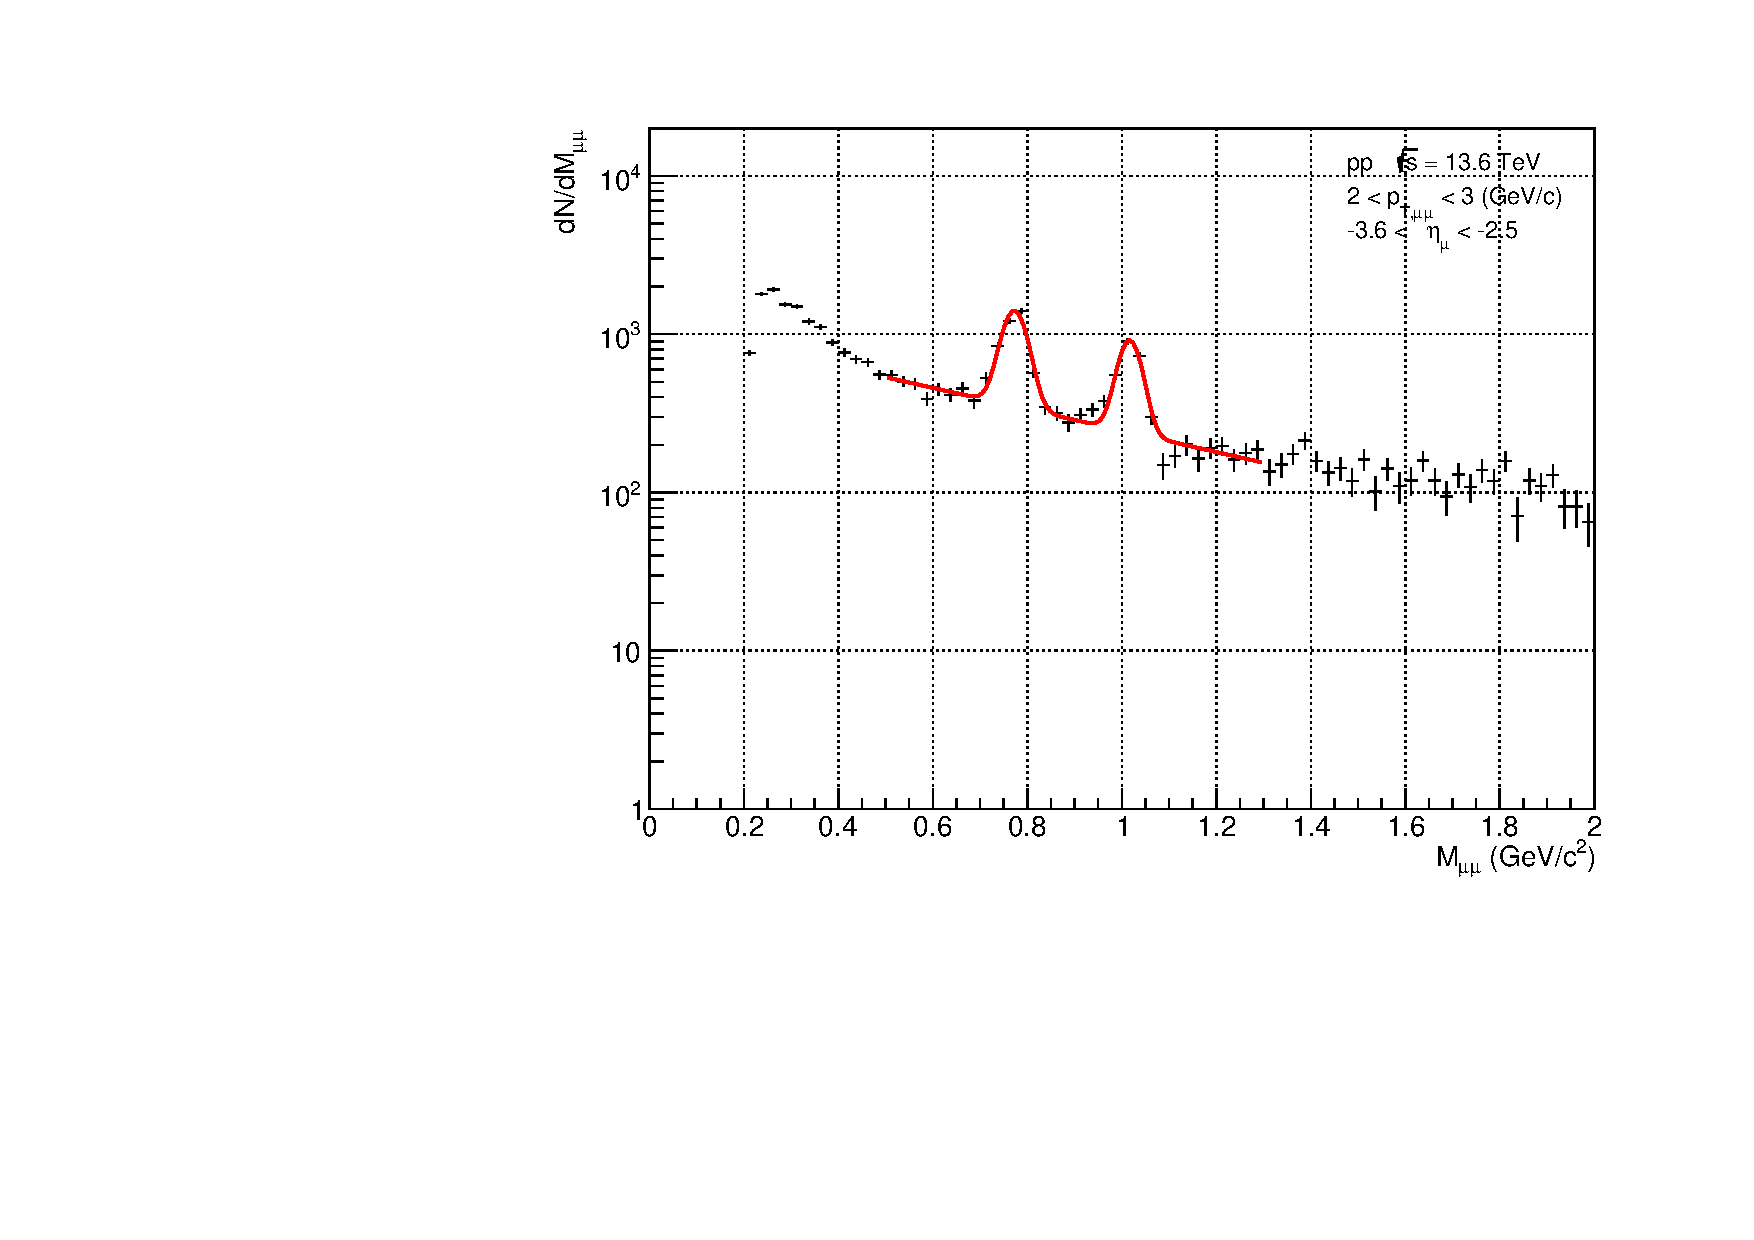
\includegraphics[width=\textwidth]{fig/3_4_2_fit_pt_2to3.pdf}
                        \captionsetup{labelformat=empty}
                        \caption*{2 < $p_{T}$ < 3}
                    \end{minipage}
                    \\
                    \vspace{1em}
                    \begin{minipage}{0.45\textwidth}
                        \centering
                        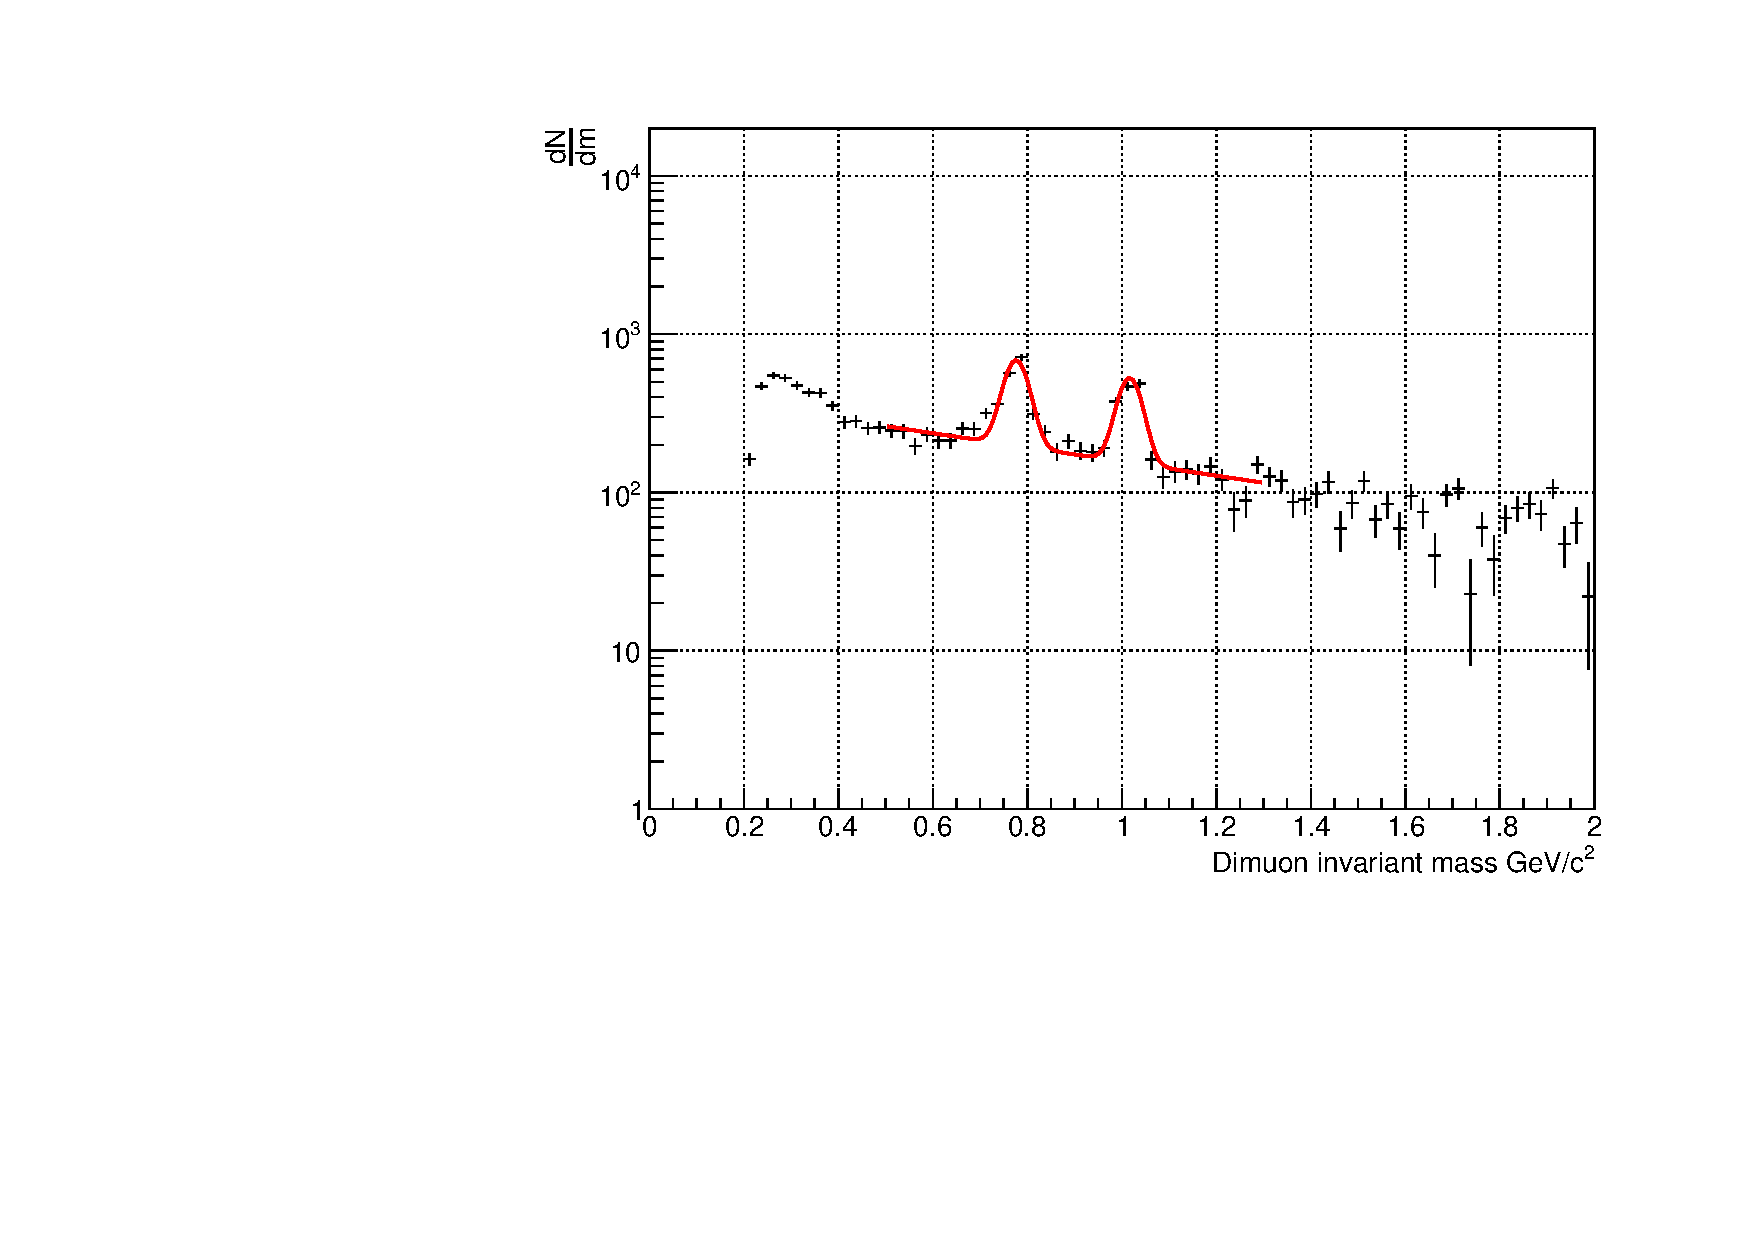
\includegraphics[width=\textwidth]{fig/3_4_2_fit_pt_3to4.pdf}
                        \captionsetup{labelformat=empty}
                        \caption*{3 < $p_{T}$ < 4}
                    \end{minipage}
                    \hfill
                    \begin{minipage}{0.45\textwidth}
                        \centering
                        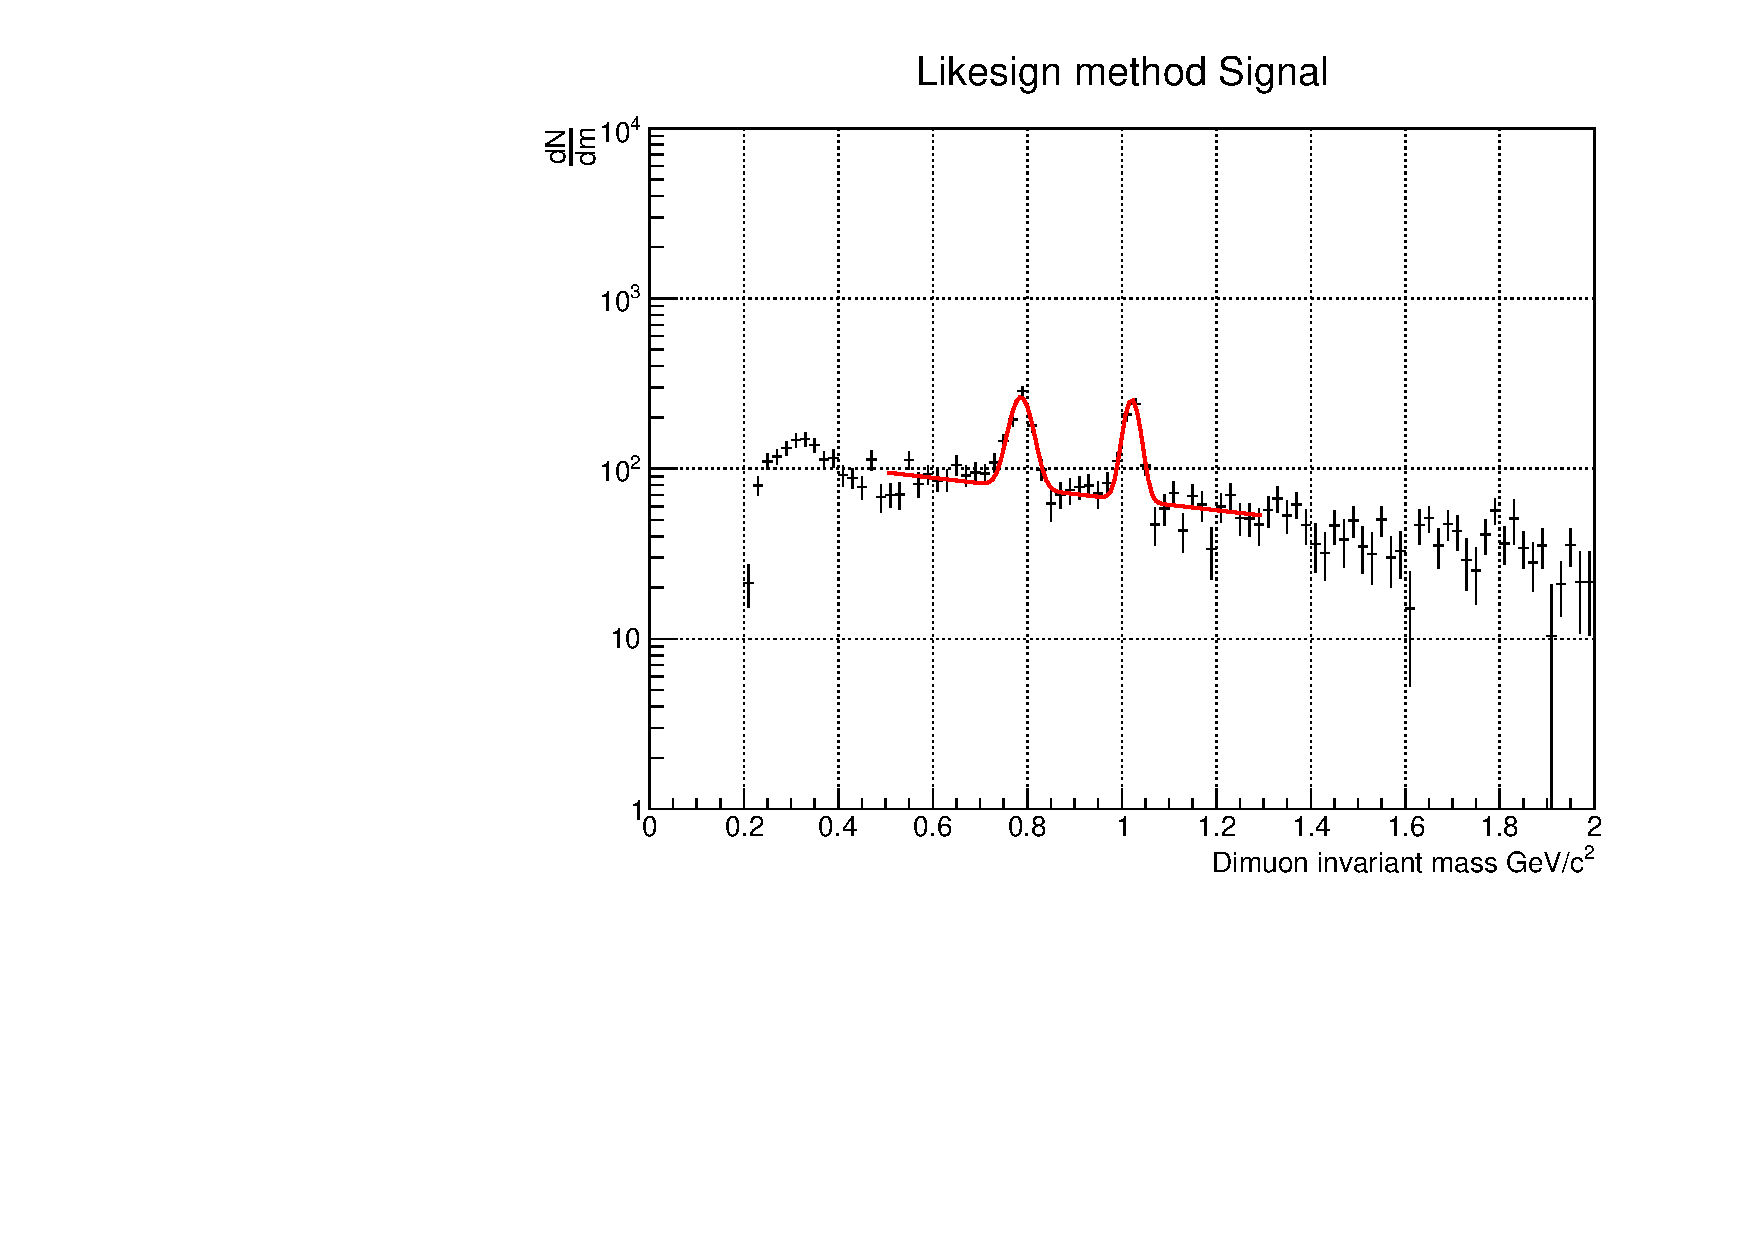
\includegraphics[width=\textwidth]{fig/3_4_2_fit_pt_4to5.pdf}
                        \captionsetup{labelformat=empty}
                        \caption*{4 < $p_{T}$ < 5} 
    
                    \end{minipage}
                    \\
                    \vspace{1em}
                    \begin{minipage}{0.45\textwidth}
                        \centering
                        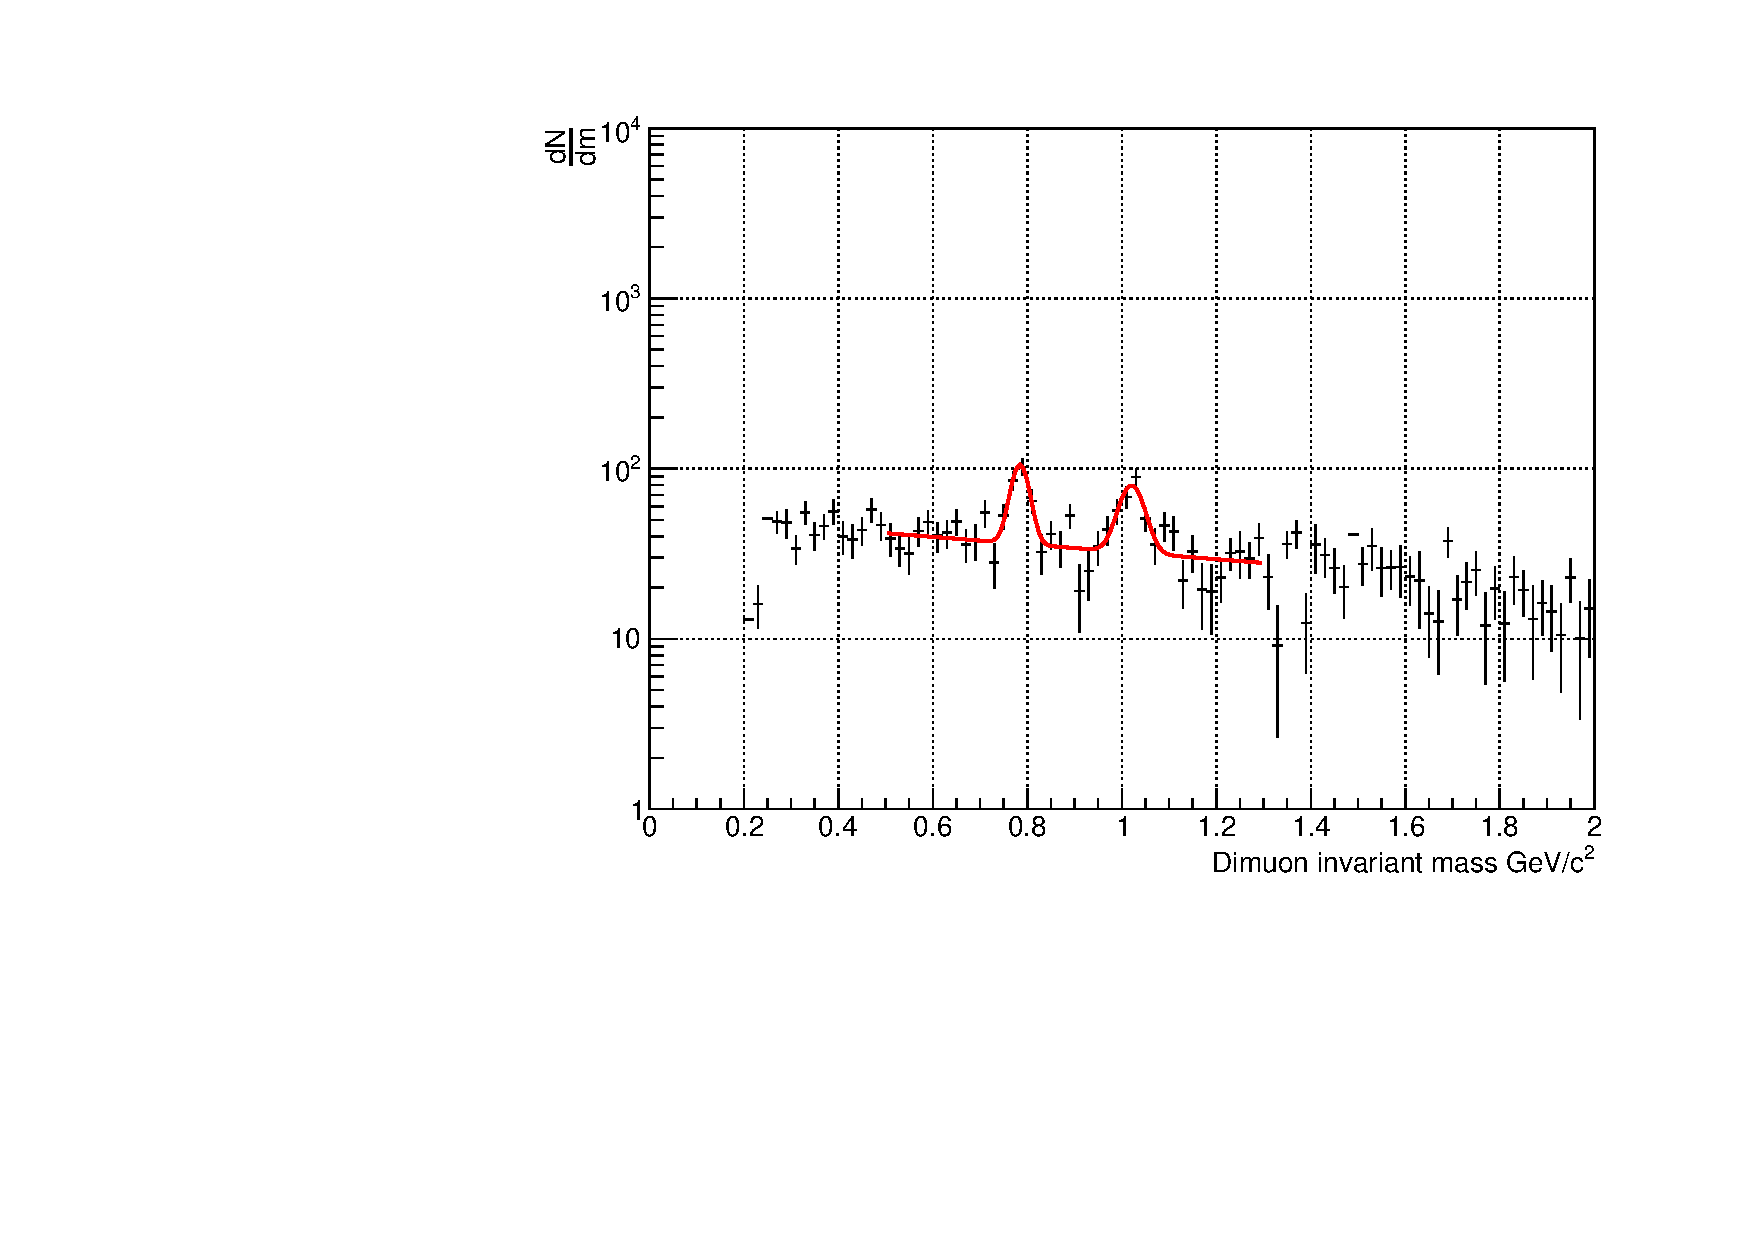
\includegraphics[width=\textwidth]{fig/3_4_2_fit_pt_5to6.pdf}
                        \captionsetup{labelformat=empty}
                        \caption*{5 < $p_{T}$ < 6}
                    \end{minipage}
                    \hfill
                    \begin{minipage}{0.45\textwidth}
                        \centering
                        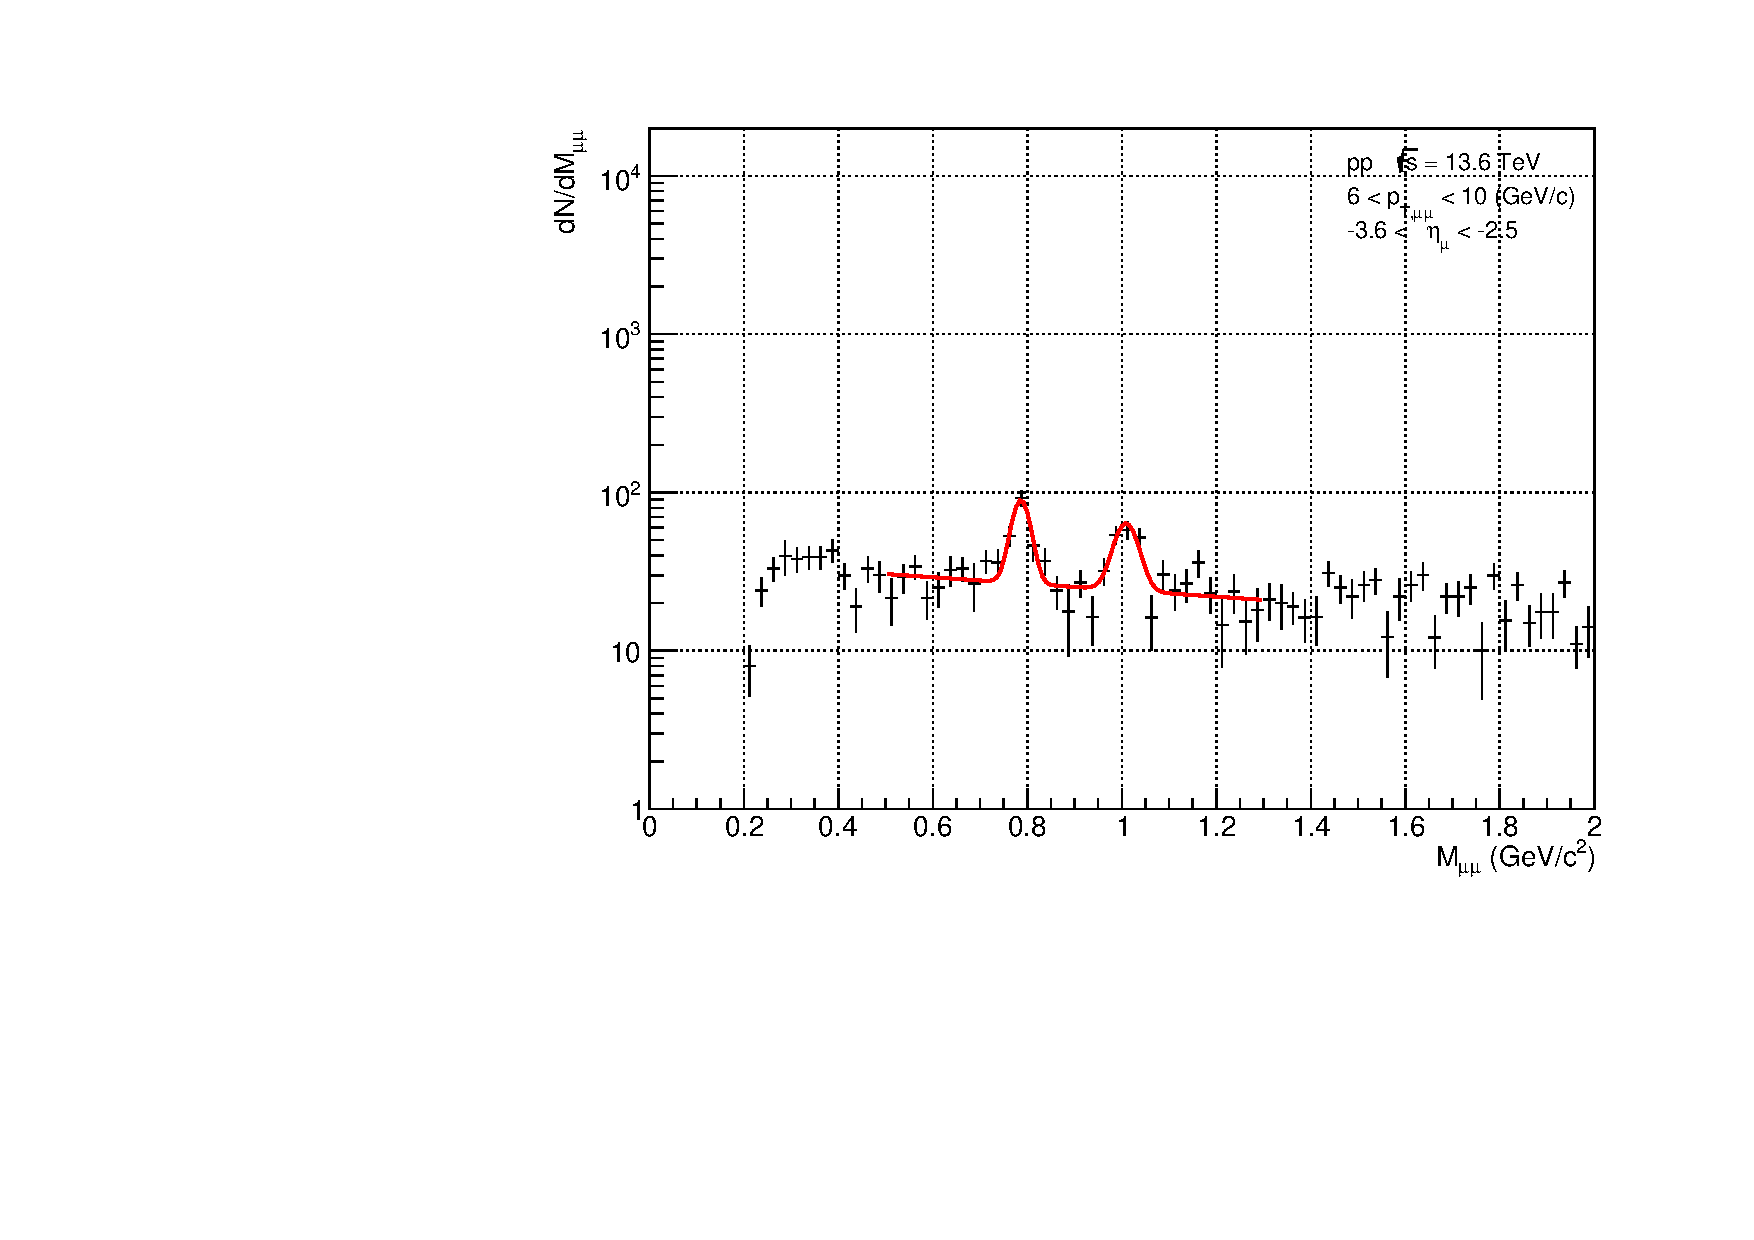
\includegraphics[width=\textwidth]{fig/3_4_2_fit_pt_6to10.pdf}
                        \captionsetup{labelformat=empty}
                        \caption*{6 < $p_{T}$ < 10}
                    \end{minipage}
                    \caption{fit result of each pt}
                    \label{Analysis:Dimuon:Yield:fit}
                \end{figure}
                The mean mass positions and mass widths of \(\omega\) and \(\phi\) for each transverse momentum, as well as the \(\chi^2\) of the fit, are summarized in the following table.
                    \begin{table}[htbp]
                        \centering
                        \caption{Fit Results}
                        \resizebox{\textwidth}{!}{
                            \begin{tabular}{|c||c|c|c|c|c|}
                                \hline
                                & $\omega$ mean mass & $\omega$ mass width & $\phi$ mean mass & $\phi$ mass width & fit $\chi^2$ \\ \hline \hline
                                1 < $p_{T}$ < 2 &$0.769\pm0.002$& $0.026\pm0.002$ &$1.01\pm0.00$ &$0.026\pm 0.003$ & 34.71/24\\ \hline
                                2 < $p_{T}$ < 3 &$0.774\pm0.001$&$0.026\pm0.001$ & $1.016\pm0.002$& $0.024\pm 0.001$ & 44.32/24\\ \hline
                                3 < $p_{T}$ < 4 &$0.776\pm0.002$& $0.025\pm0.002$ &$1.017\pm0.002$ &$0.025\pm 0.001$ & 71.93/24\\ \hline
                                4 < $p_{T}$ < 5 &$0.787\pm0.002$& $0.023\pm0.002$ &$1.02\pm0.00$ &$0.021\pm 0.002$ & 45.63/24\\ \hline
                                5 < $p_{T}$ < 6 &$0.787\pm0.003$& $0.018\pm0.003$ &$1.02\pm0.005$ &$0.027\pm 0.006$ & 41.72/24\\ \hline
                                6 < $p_{T}$ < 10 &$0.787\pm0.004$& $0.021\pm0.005$ &$1.01\pm0.01$ &$0.025\pm 0.004$ & 16.18/22\\ \hline
                            \end{tabular}
                        }
                        \label{Analysis:Dimuon:Yield:Fit_Results}
                    \end{table}
        \subsubsection{Yield calculation of $\omega,\phi$} 
            Using the mean mass position and mass width of $\omega \rightarrow \mu\mu$ and $\phi \rightarrow \mu\mu$ obtained from the above fit, the yield for each meson was calculated. The number of dimuons falling within 3$\sigma$ of each Gaussian was calculated as the yield for $\omega$ and $\phi$, respectively.
            \begin{eqnarray}
                \mathrm{min} &=&  -3 \times \sigma + M \\
                \mathrm{max} &=&  3 \times \sigma + M \\
                \mathrm{Yield} &=& \sum_{\mathrm{min}}^{\mathrm{max}} F(m)
                \label{Yield:calculation}
            \end{eqnarray}
            Using the mean mass positions and mass widths of \(\omega \rightarrow \mu\mu\) and \(\phi \rightarrow \mu\mu\) obtained from the above fit, the yields for each were calculated. The mass distribution, obtained by subtracting the continuous component from the dimuon mass distribution with correlations, was used. For this mass distribution, the number of entries within three times the mass width from the mass positions of \(\omega\) and \(\phi\) were calculated as their respective yields. The calculation formula is as (\ref{Yield:calculation}), where the mass distribution after subtracting the continuous component is denoted as \(F(m)\).
            \begin{table}[htbp]
                \centering
                \caption{Fit Results}
                \begin{tabular}{|c||c|c|}
                    \hline
                    & $\omega$ Yield & $\phi$ Yield \\ \hline \hline
                    1 < $p_{T}$ < 2 &$(3.00\pm0.24)\times10^3$& $(1.83\pm0.21)\times10^3$\\ \hline
                    2 < $p_{T}$ < 3 &$(3.11\pm0.14)\times10^3$& $(1.75\pm0.11)\times10^3$\\ \hline
                    3 < $p_{T}$ < 4 &$(1.331\pm0.070)\times10^3$& $(0.902\pm0.062)\times10^3$\\ \hline
                    4 < $p_{T}$ < 5 &$(0.538\pm0.042)\times10^3$& $(0.387\pm0.037)\times10^3$\\ \hline
                    5 < $p_{T}$ < 6 &$(0.150\pm0.022)\times10^3$& $(0.144\pm0.024)\times10^3$\\ \hline
                    6 < $p_{T}$ < 10 &$(0.037\pm0.0057)\times10^3$& $(0.023\pm0.050)\times10^3$\\ \hline     
                \end{tabular}
                \label{Analysis:Dimuon:Yield:Results}
            \end{table}
            The results from the table above are presented as graphs in \ref{fig:omega_yield} and \ref{fig:phi_yield}.

    \subsection{Analysis for improving MFT-MCH matching purity}
        The mass distribution of dimuons with \( p_T \) below 1 GeV, which is not shown in \ref{Analysis:Dimuon:CB:CB_pt_separation}, is presented here.
        \begin{figure}
            \centering
            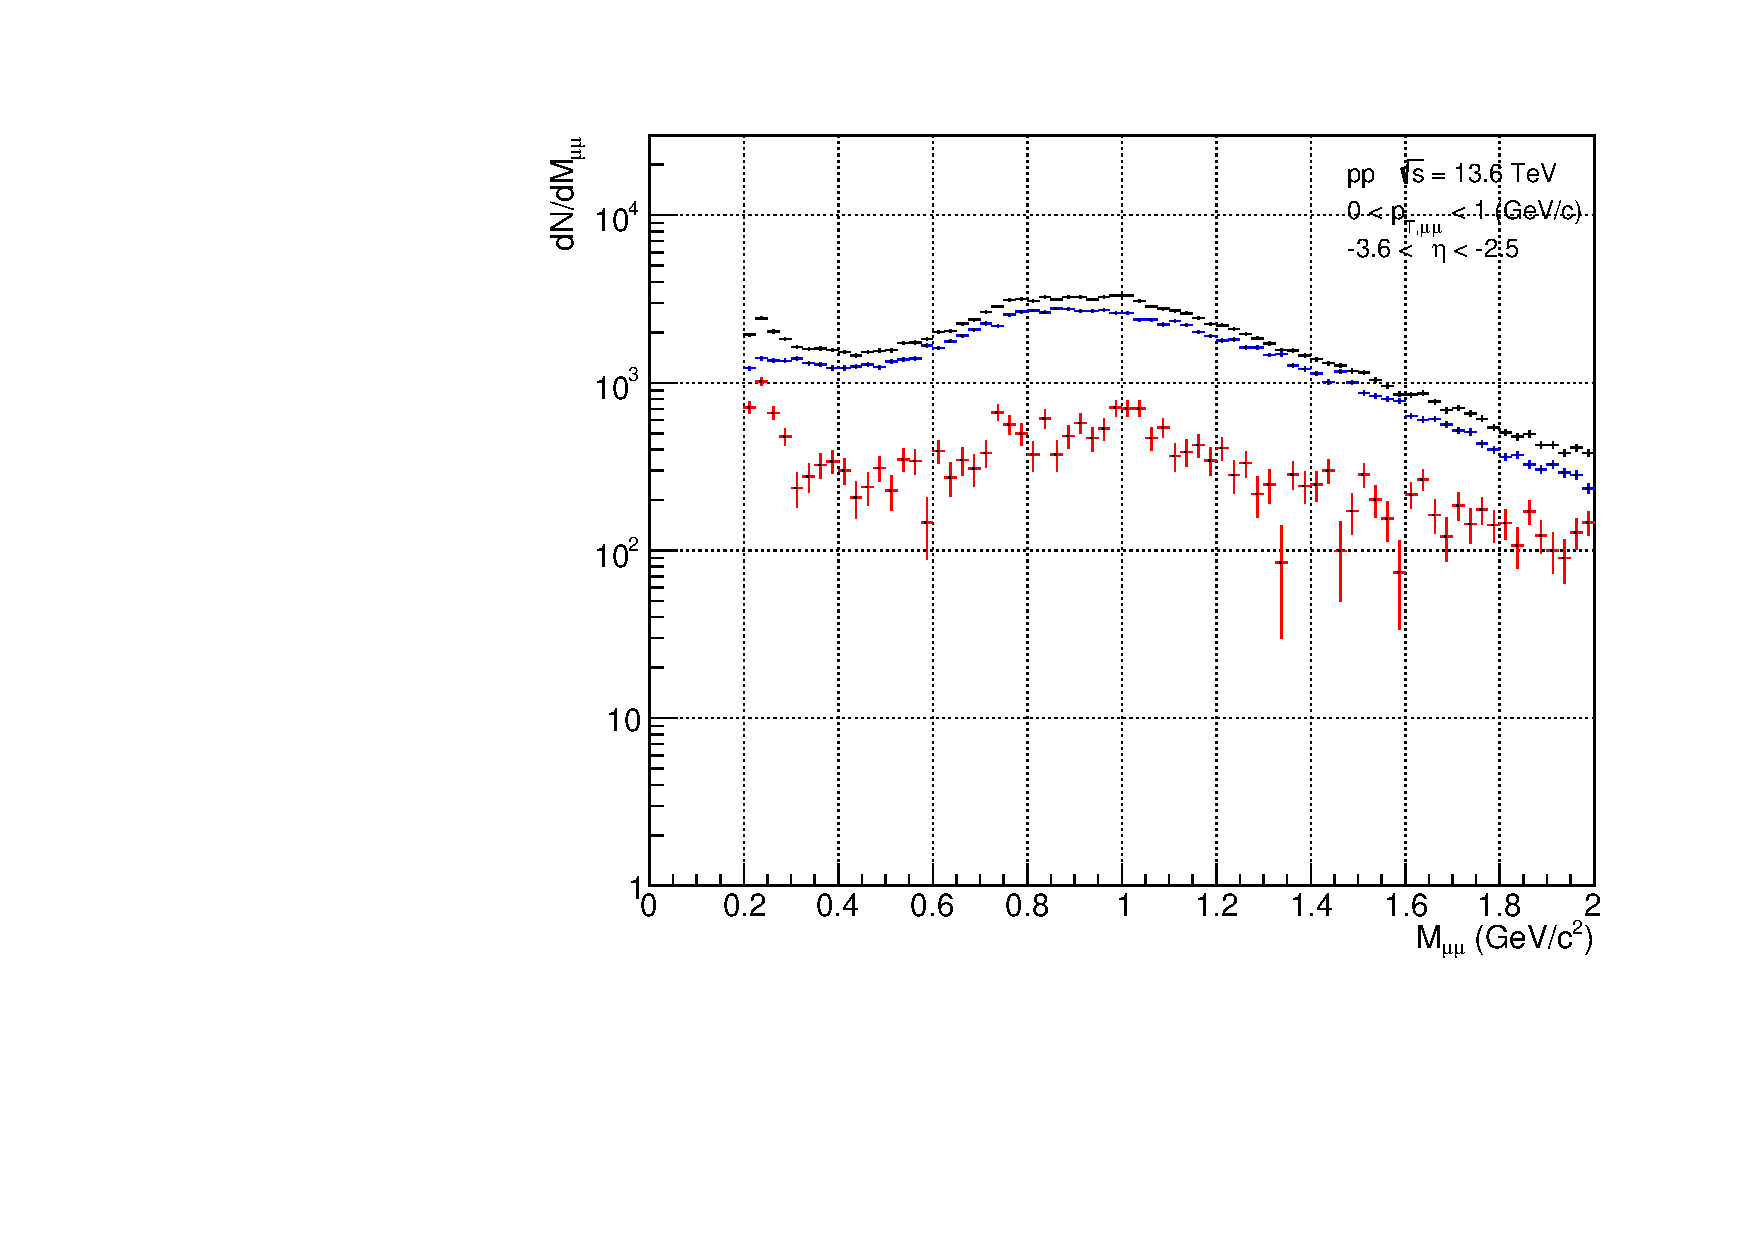
\includegraphics[keepaspectratio, scale=0.4]{fig/3_6_CB_pt0to1.pdf}
            \caption{Combinatorial subtraction of dimuon transverse momentum 0 < $p_T$ < 1}
            \label{Analysis:Dimuon:pt0to1}
        \end{figure}
        From \ref{Analysis:Dimuon:pt0to1}, the peak structures of \(\omega\) and \(\phi\) could not be measured. This is due to the insufficient reconstruction resolution of \(\eta\), \(p_T\), and \(\phi\) at low \(p_T\) for single muons. The introduction of the MFT is expected to enable high-precision measurements of \(\eta\) and \(\phi\), which would improve the reconstruction resolution of \(p_T\) through enhanced \(\eta\) and \(\phi\) resolution. However, with the current reconstruction method, sufficient resolution has not been achieved, resulting in the inability to observe the peaks of \(\omega\) and \(\phi\) in the dimuon invariant mass distribution at low transverse momentum. This can likely be attributed to issues in the matching between tracks from the newly introduced MFT and those from the MCH, which prevent achieving adequate resolution. In this chapter, we present an analysis aimed at improving the MFT-MCH matching purity across all transverse momentum distributions, without restricting to low \(p_T\).

        \subsubsection{MFT-MCH matching $\chi^2$ Optimization}
        \label{matching_chi2_opt}
            Using the yield analysis method for \(\omega \rightarrow \mu\mu, \phi \rightarrow \mu\mu\) described in \ref{Analysis:Dimuon:Combinatorial BG subtraction}-\ref{Analysis:Dimuon:Yieldcal}, the MFT-MCH matching \(\chi^2\) cut value for single muon tracks was optimized to maximize signal detection efficiency. The MFT-MCH matching \(\chi^2\) value represents the difference in parameters when extrapolating MFT and MCH tracks to the matching plane. A larger \(\chi^2\) value tends to indicate more fake matches, whereas a smaller value corresponds to more correct matches. By applying a cut on this value, fake match tracks can be removed. however, it is necessary to optimize the cut to minimize fake matches while preserving as many correct matches as possible. In this study, the optimization was performed by maximizing the signal significance using the peaks of \(\omega\) and \(\phi\).
            The signal was calculated by performing the same analysis as in \ref{Analysis:Dimuon:Combinatorial BG subtraction}, \ref{Peak_extraction}, and \ref{Analysis:Dimuon:Yieldcal} for the mass distributions in all transverse momentum regions. The number of background events was determined by counting the entries in the background-subtracted mass distribution within the same mass window used for signal calculation, and this was used as the background estimate. The significance, \( S/\sqrt{S+BG} \), was then calculated. This calculation was performed for mass distributions reconstructed using only muons with an MFT-MCH matching \(\chi^2\) below a given threshold.  
            Fig. \ref{Analysis:Dimuon:Matching_CB} presents the results of the combinatorial background subtraction after applying the \(\chi^2\) cut. Similar to \ref{Analysis:Dimuon:CB:CB_pt_separation}, the black histogram represents the mass distribution reconstructed from all oppositely charged muon pairs in the same event, while the blue histogram represents the combinatorial background estimated using the Like Sign method. The red histogram corresponds to the background-subtracted distribution, representing the invariant mass distribution of correlated dimuons.
            \begin{figure}[H]
                \centering
                \begin{minipage}{0.45\textwidth}
                    \centering
                    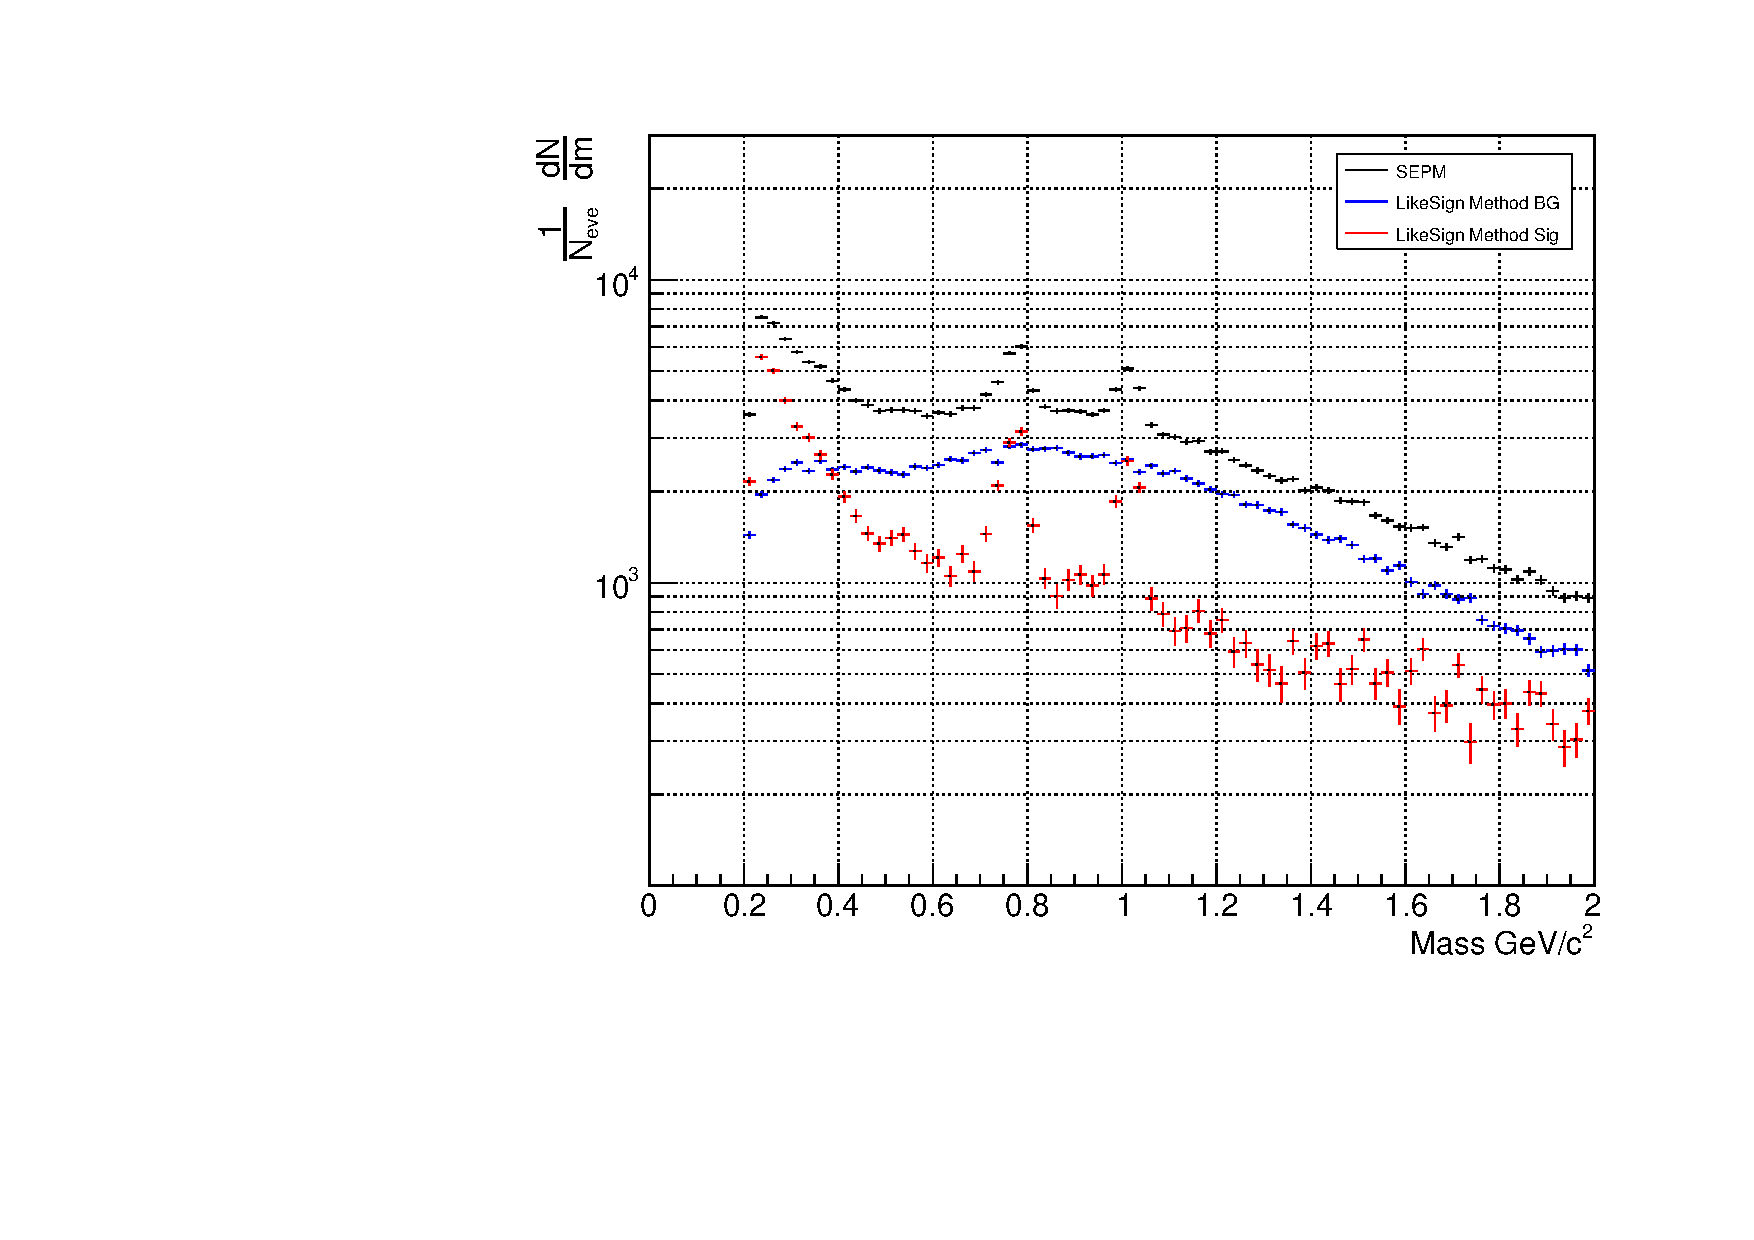
\includegraphics[width=\textwidth]{fig/3_4_4_CB_chi2_20.pdf}
                    \caption*{MFT-MCH matching $\chi^2 < 20$}
                \end{minipage}
                \hfill
                \begin{minipage}{0.45\textwidth}
                    \centering
                    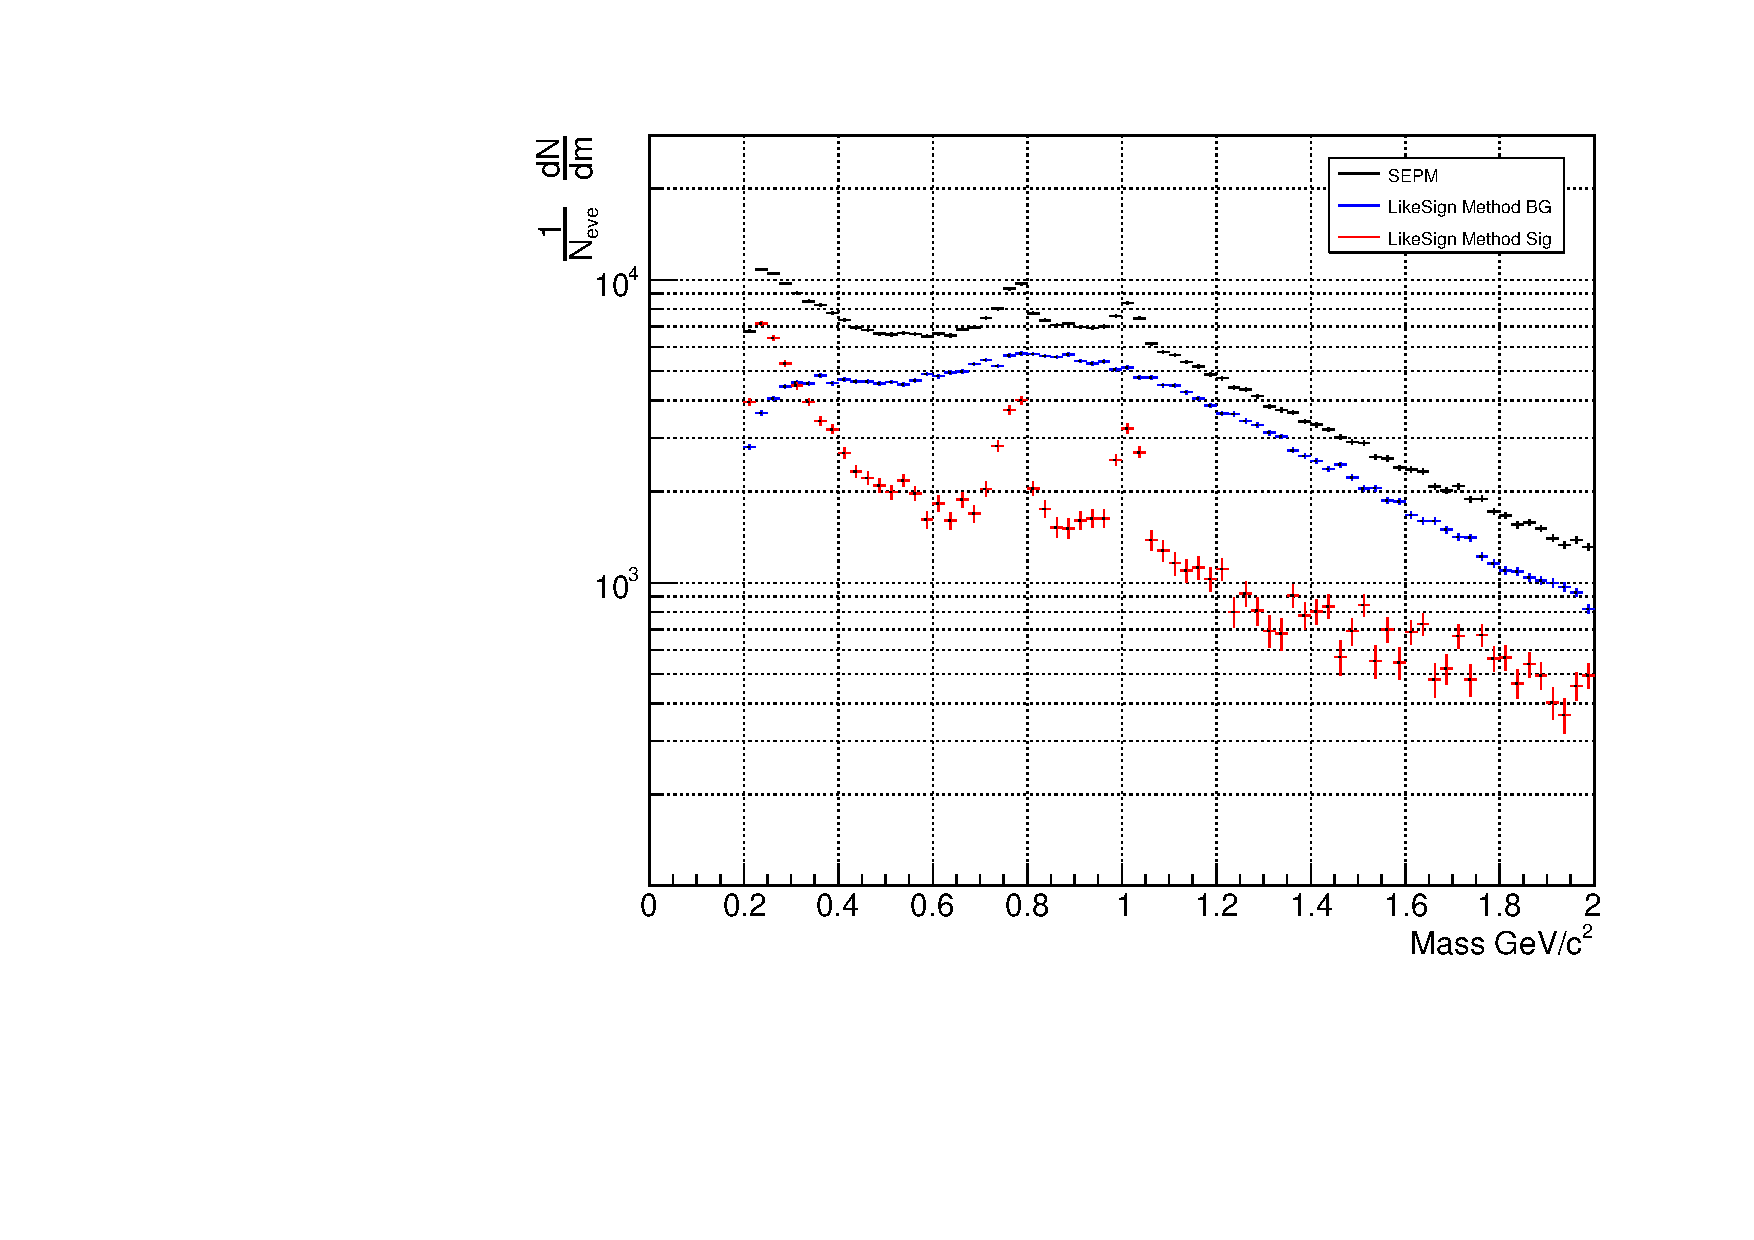
\includegraphics[width=\textwidth]{fig/3_4_4_CB_chi2_40.pdf}
                    \caption*{MFT-MCH matching $\chi^2 < 40$}
                \end{minipage}
                \\
                \vspace{1em}
                \begin{minipage}{0.45\textwidth}
                    \centering
                    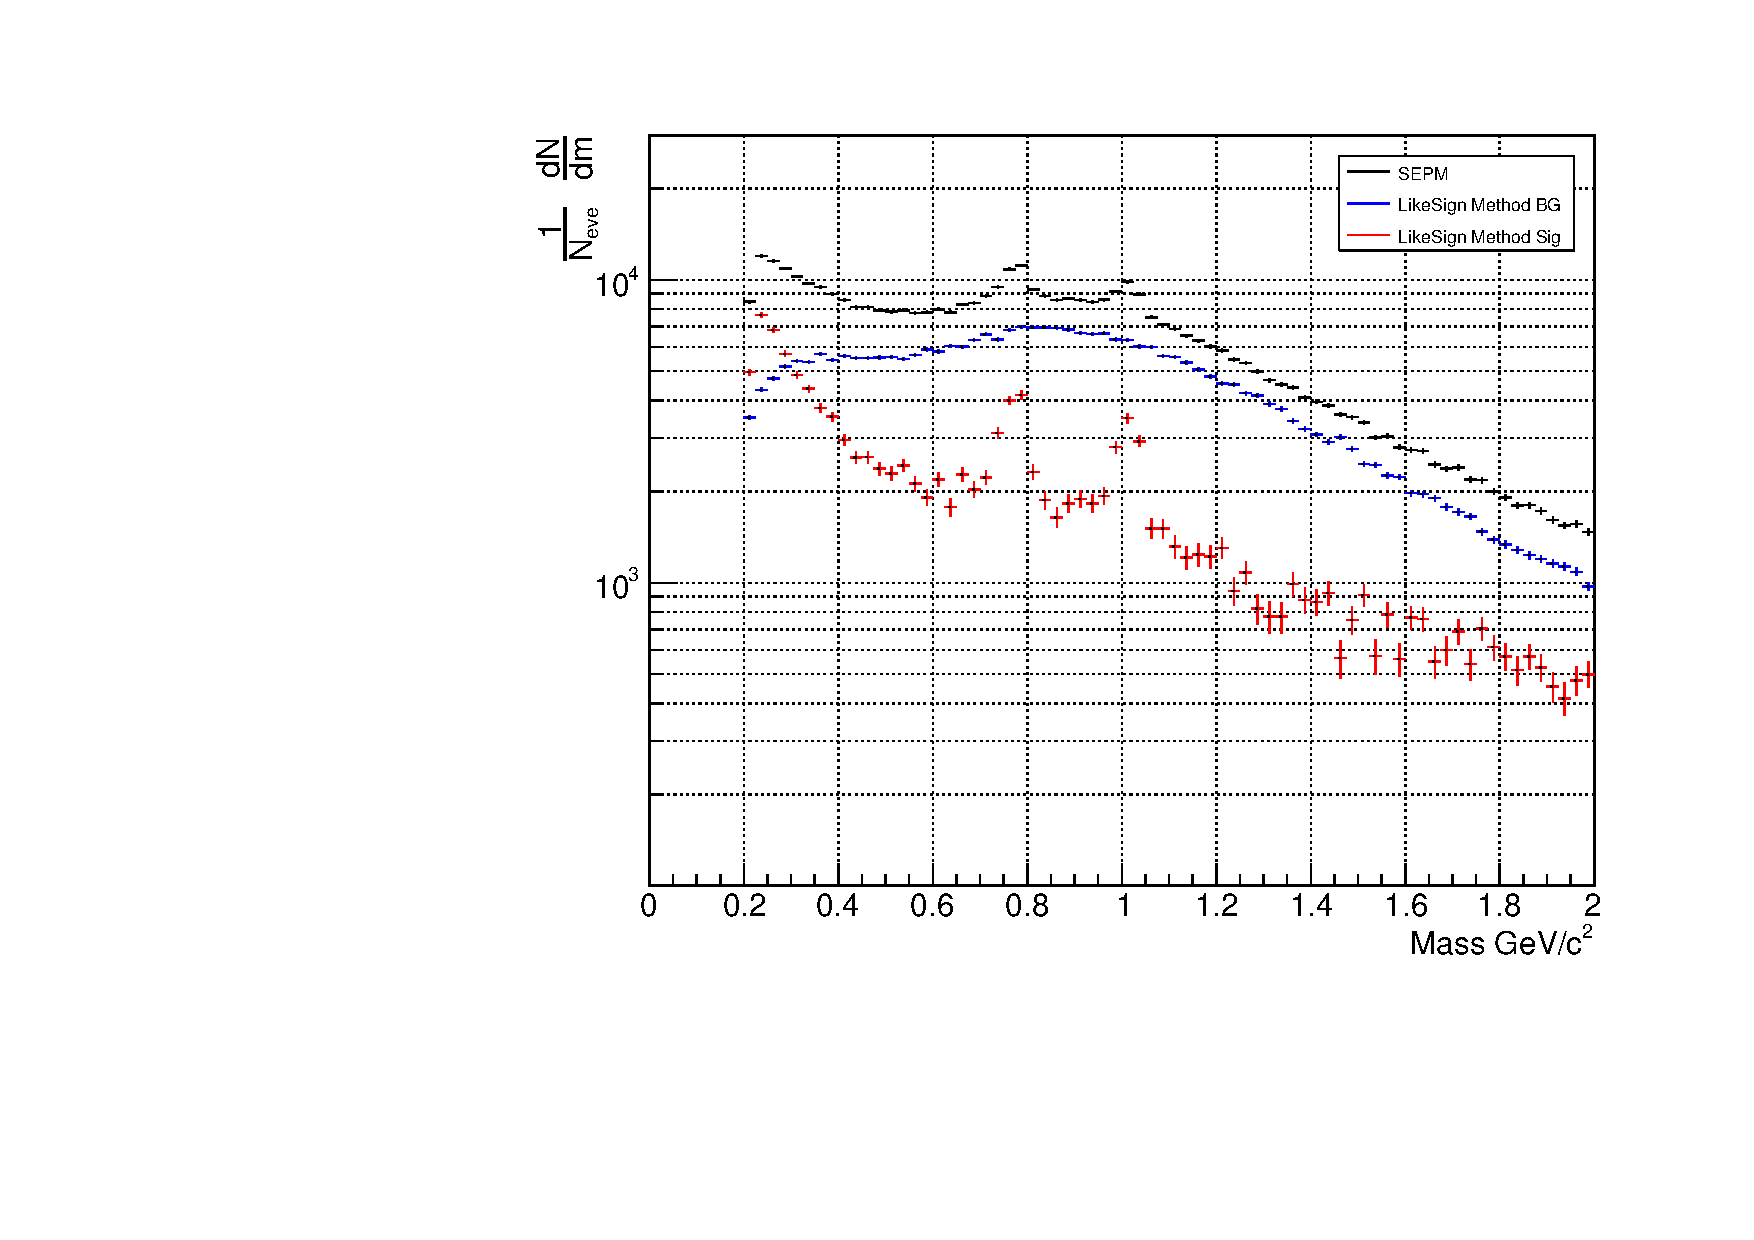
\includegraphics[width=\textwidth]{fig/3_4_4_CB_chi2_60.pdf}
                    \caption*{MFT-MCH matching $\chi^2 < 60$}
                \end{minipage}
                \hfill
                \begin{minipage}{0.45\textwidth}
                    \centering
                    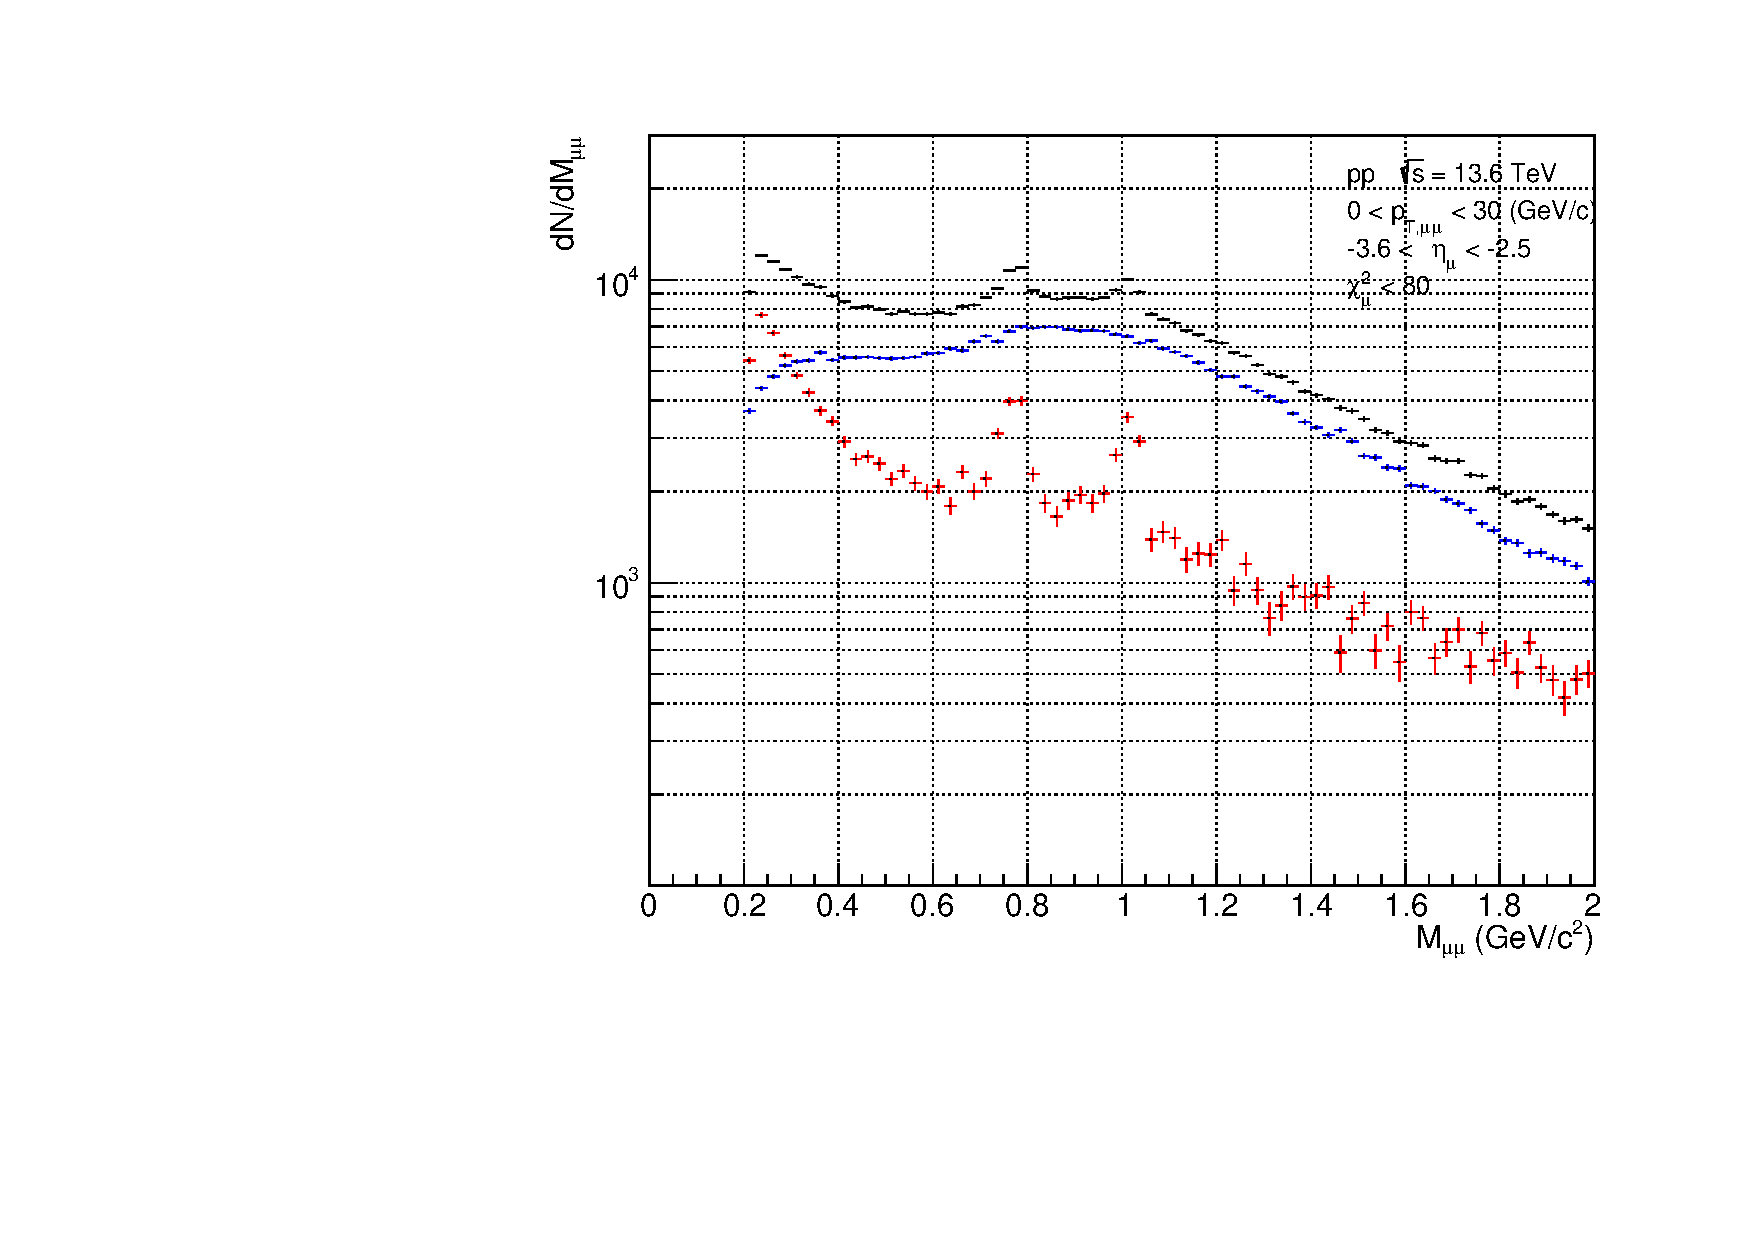
\includegraphics[width=\textwidth]{fig/3_4_4_CB_chi2_80.pdf}
                    \caption*{MFT-MCH matching $\chi^2 < 80$} 
             
                \end{minipage}
                \\
                \vspace{1em}
                \begin{minipage}{0.45\textwidth}
                    \centering
                    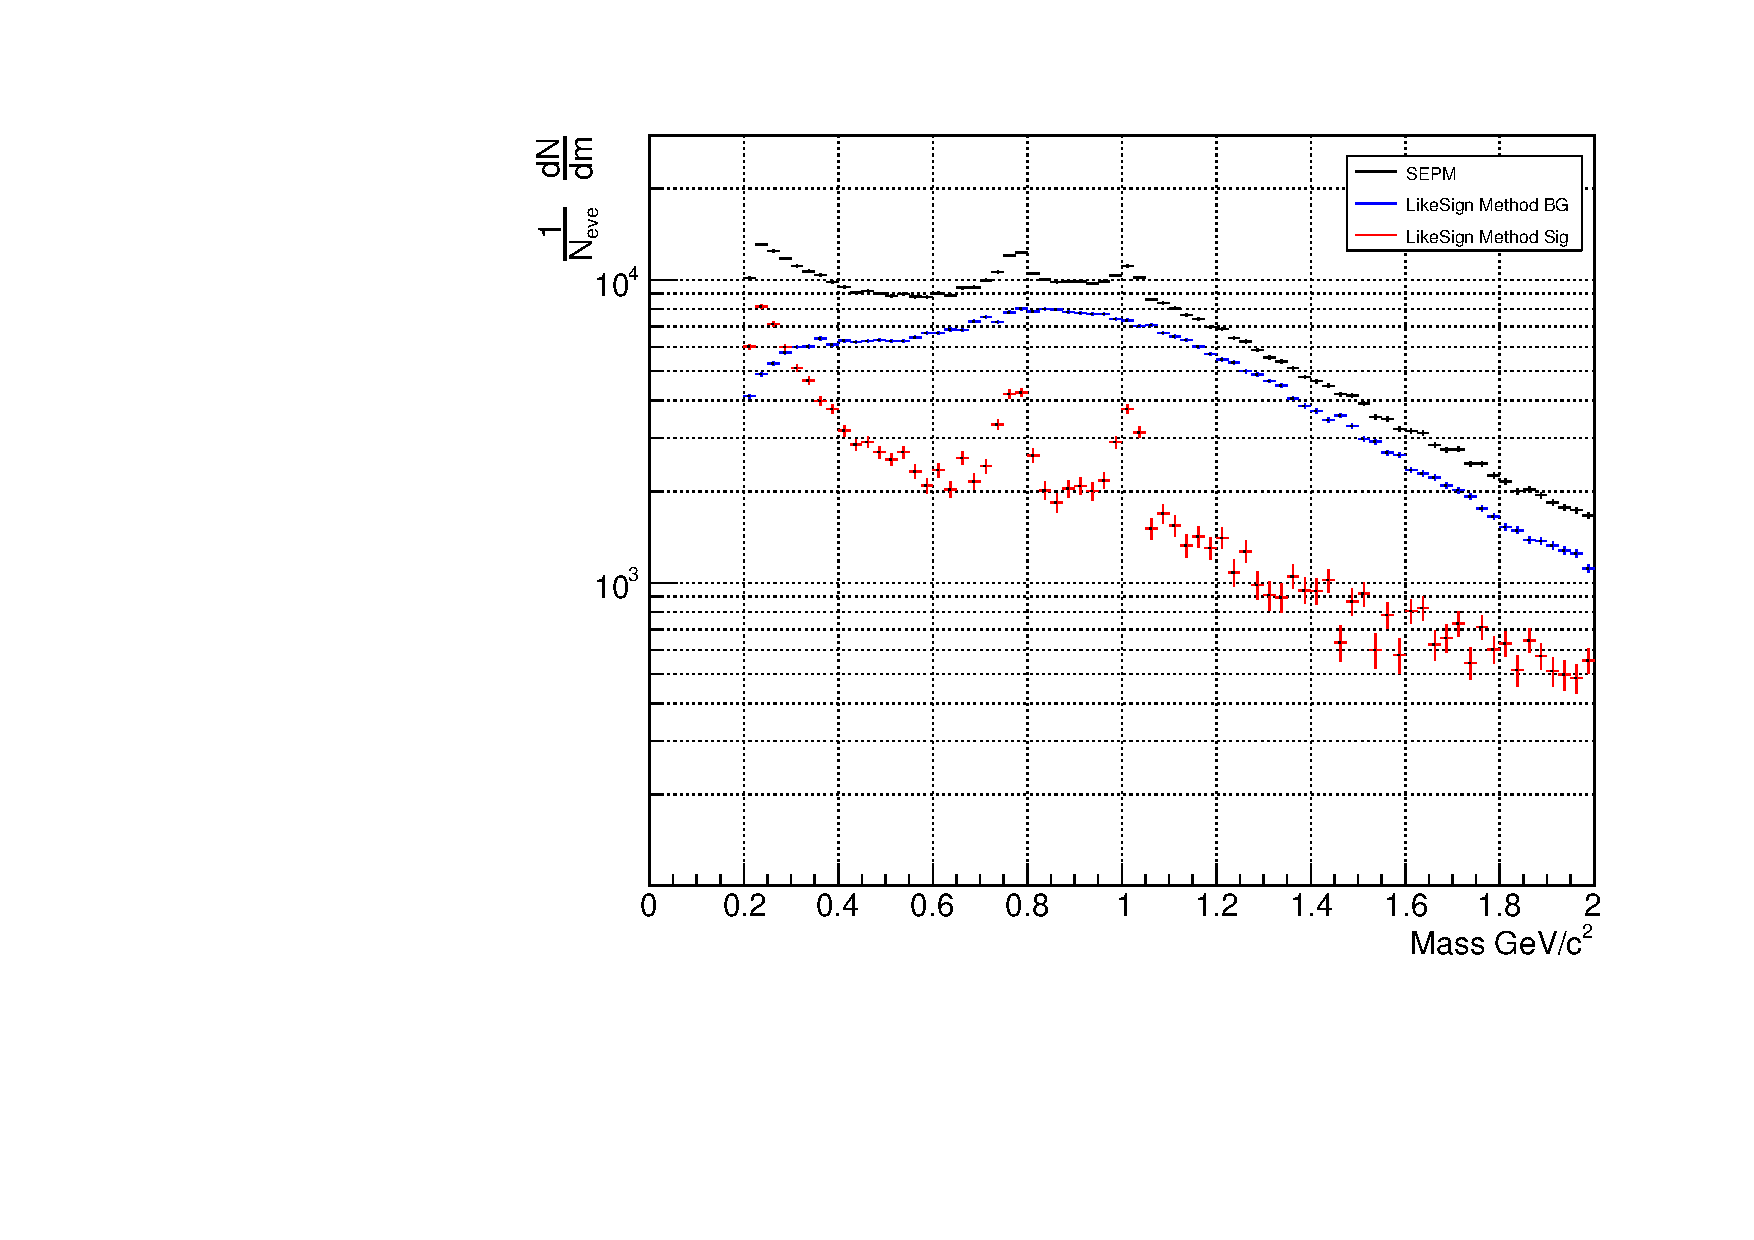
\includegraphics[width=\textwidth]{fig/3_4_4_CB_chi2_100.pdf}
                    \caption*{MFT-MCH matching $\chi^2 < 100$}
                \end{minipage}
                \hfill
                \begin{minipage}{0.45\textwidth}
                    \centering
                    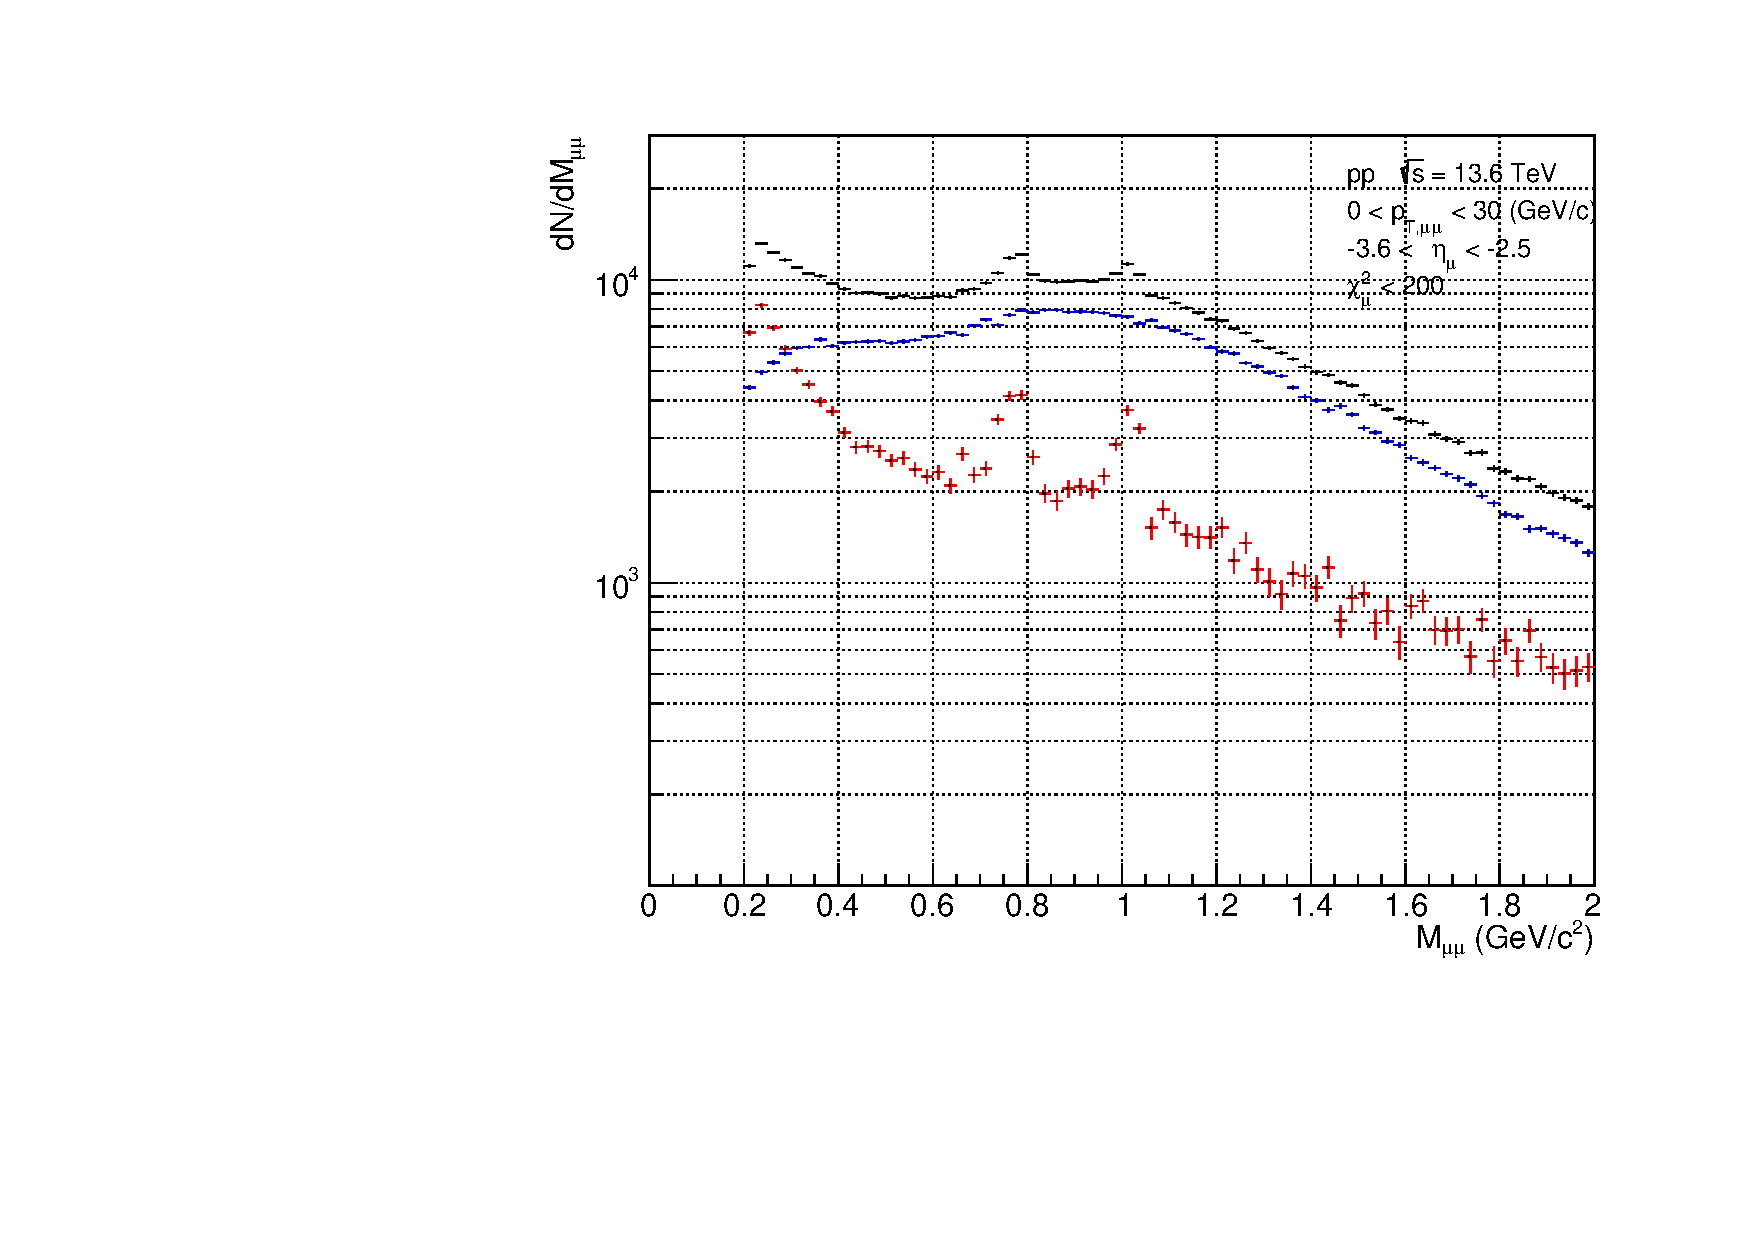
\includegraphics[width=\textwidth]{fig/3_4_4_CB_chi2_200.pdf}
                    \caption*{MFT-MCH matching $\chi^2 < 200$}
                \end{minipage}
                \caption{The result of Combinatorial Background subtraction after applying the MFT-MCH matching $\chi^2$ cut}
                \label{Analysis:Dimuon:Matching_CB}
            \end{figure}
            By reducing the \(\chi^2\) cut, the black distribution decreases in size. Additionally, it can be observed that the \(\omega\) and \(\phi\) peaks in the red distribution become more pronounced. The fitting results for this red distribution are shown in the Fig.\ref{Analysis:Dimuon:Matching_Fit}.
            \begin{figure}[H]
                \centering
                \begin{minipage}{0.45\textwidth}
                    \centering
                    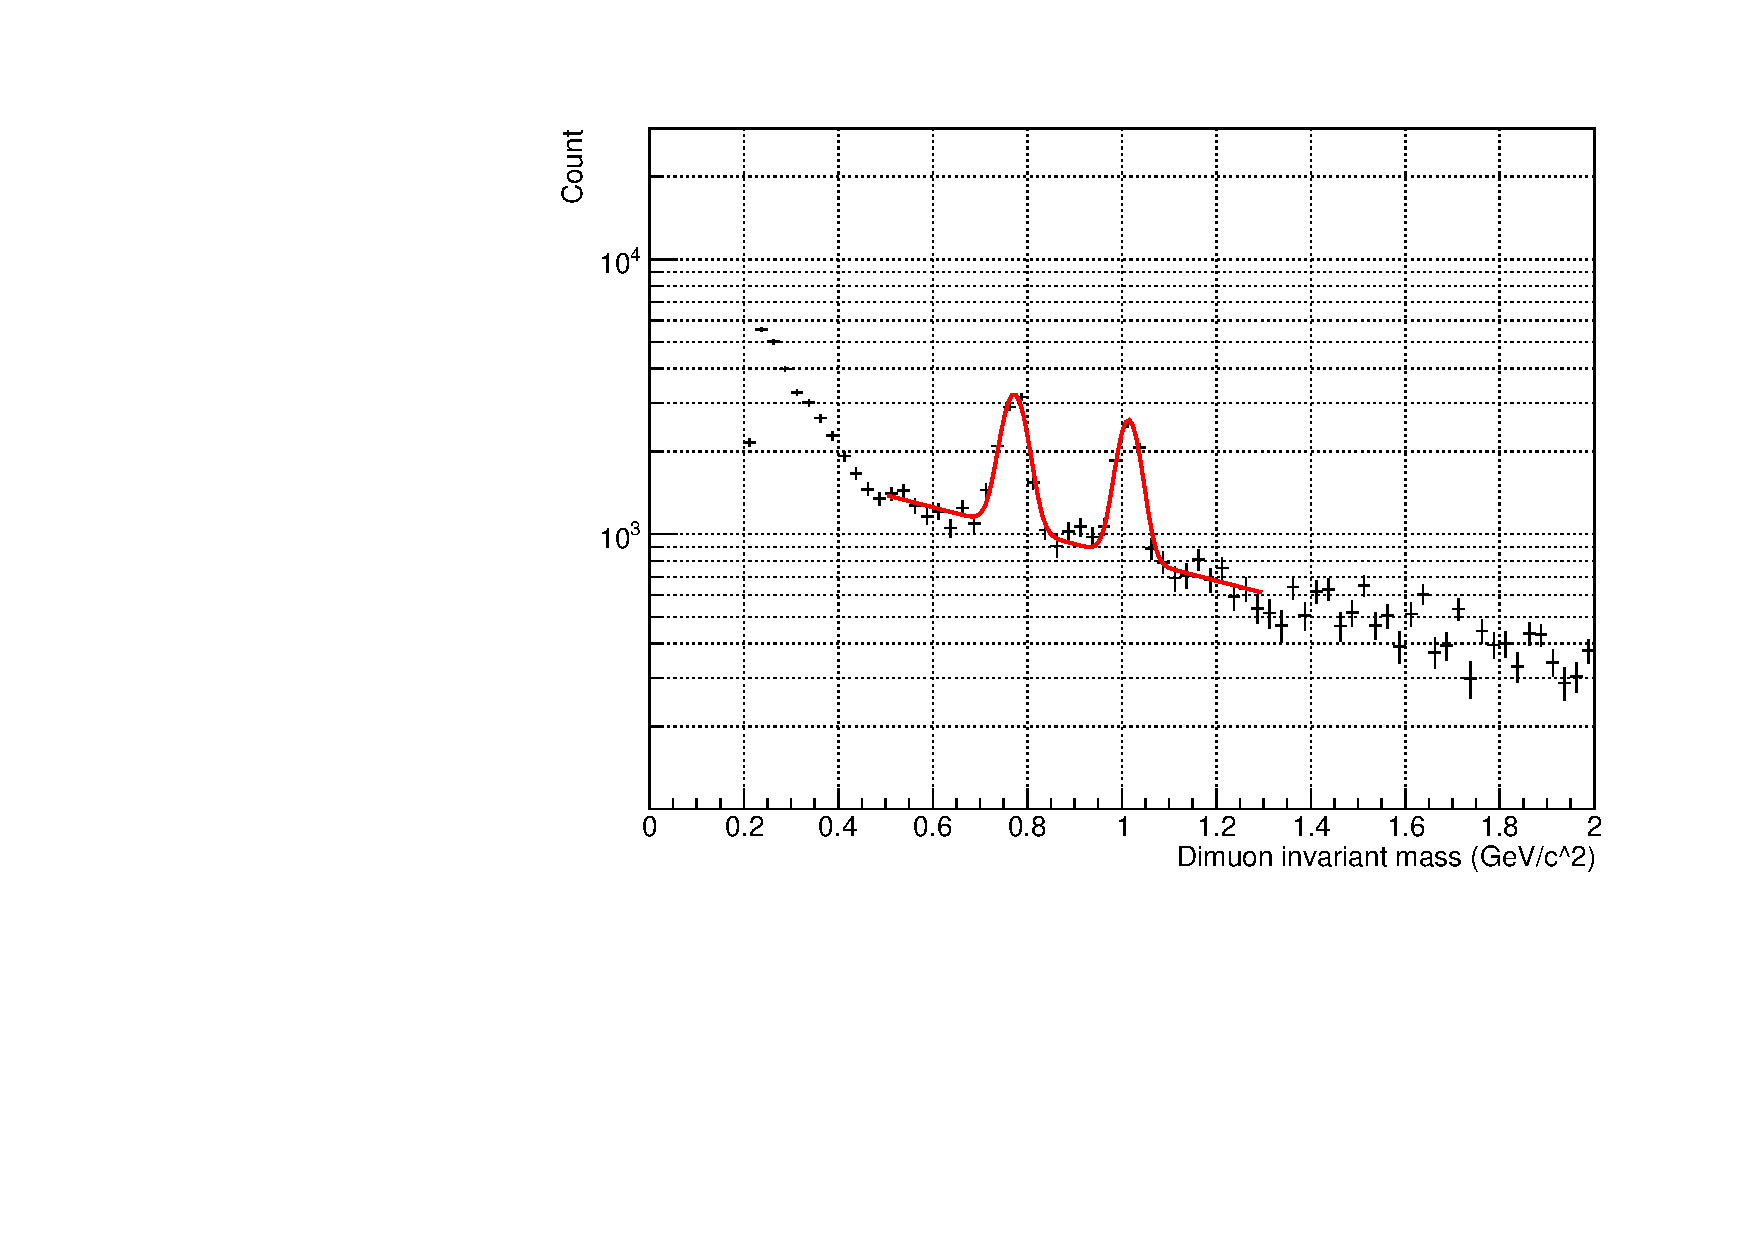
\includegraphics[width=\textwidth]{fig/3_4_4_Fit_chi2_20.pdf}
                    \caption*{MFT-MCH matching $\chi^2 < 20$}
                \end{minipage}
                \hfill
                \begin{minipage}{0.45\textwidth}
                    \centering
                    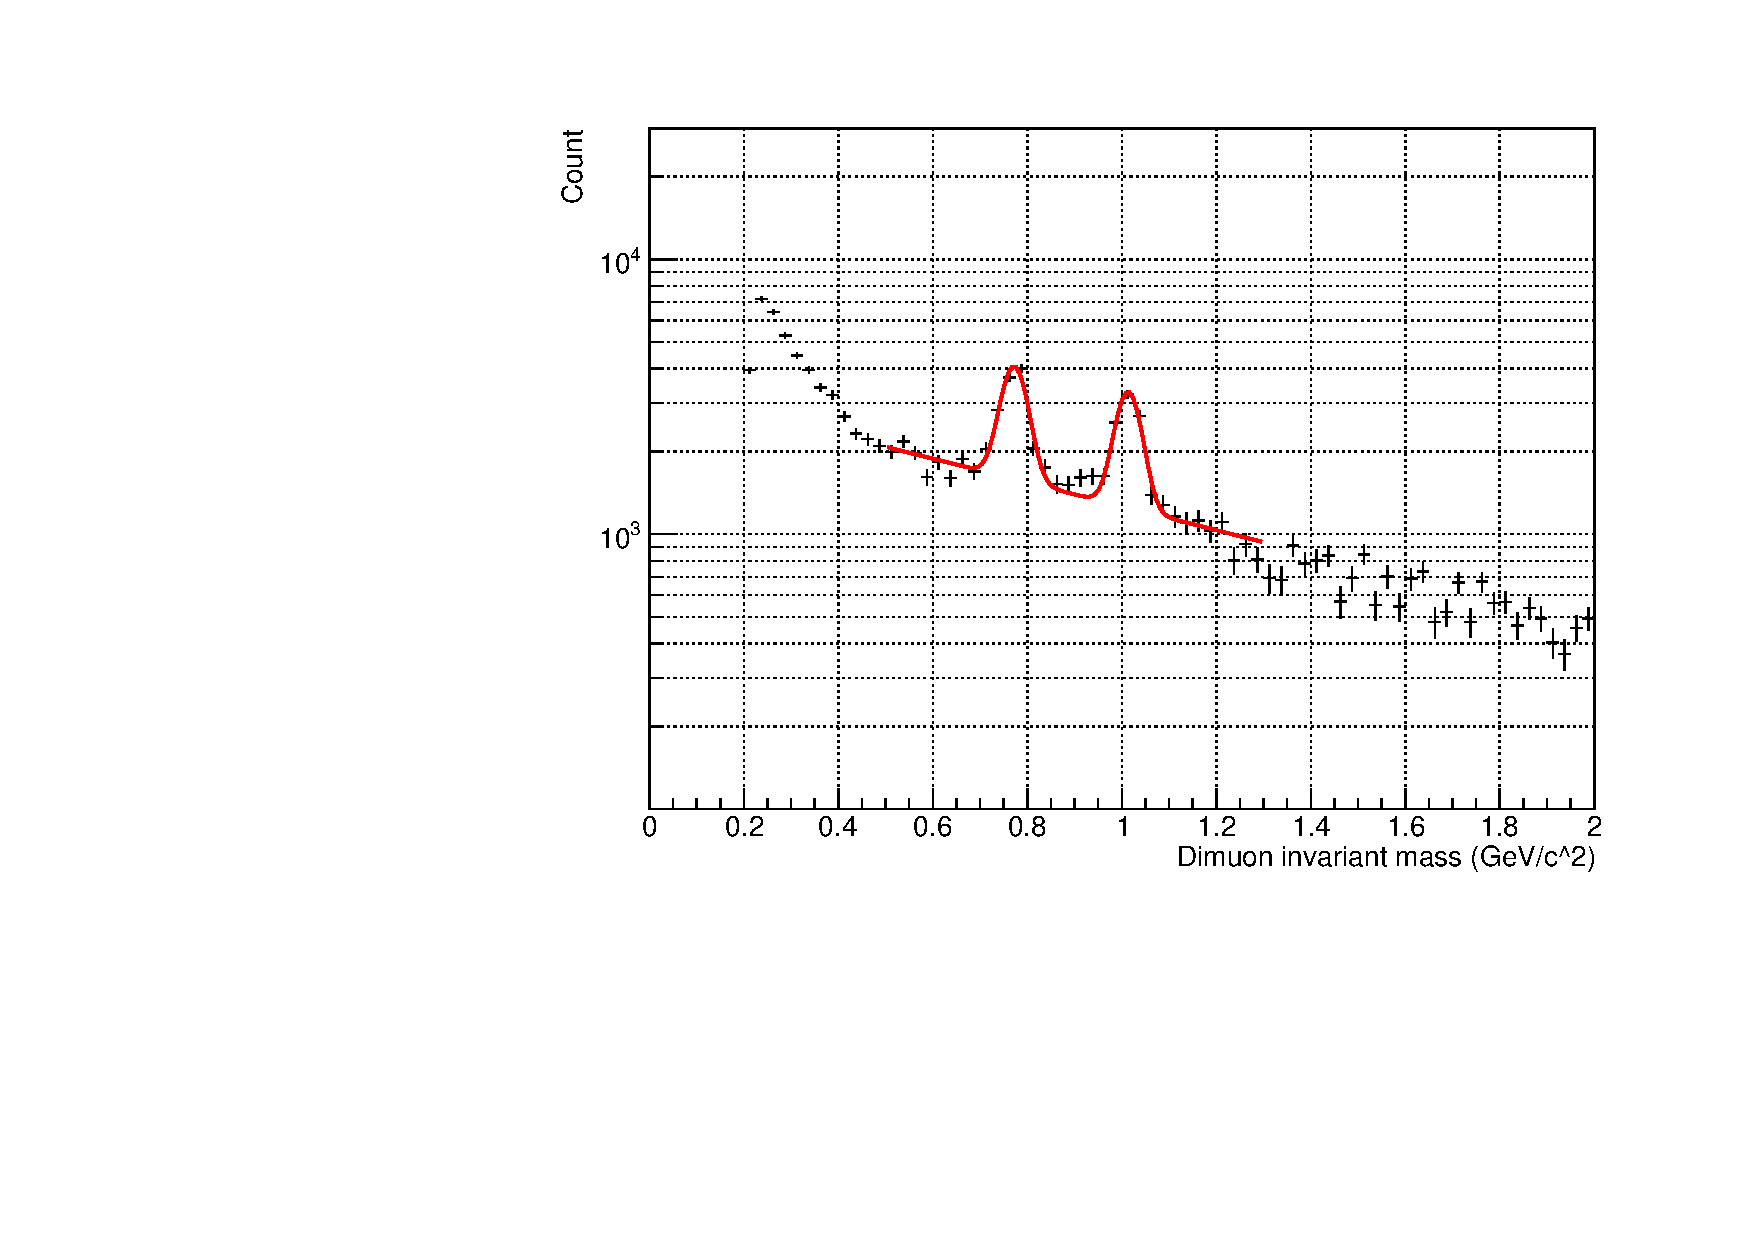
\includegraphics[width=\textwidth]{fig/3_4_4_Fit_chi2_40.pdf}
                    \caption*{MFT-MCH matching $\chi^2 < 40$}
                \end{minipage}
                \\
                \vspace{1em}
                \begin{minipage}{0.45\textwidth}
                    \centering
                    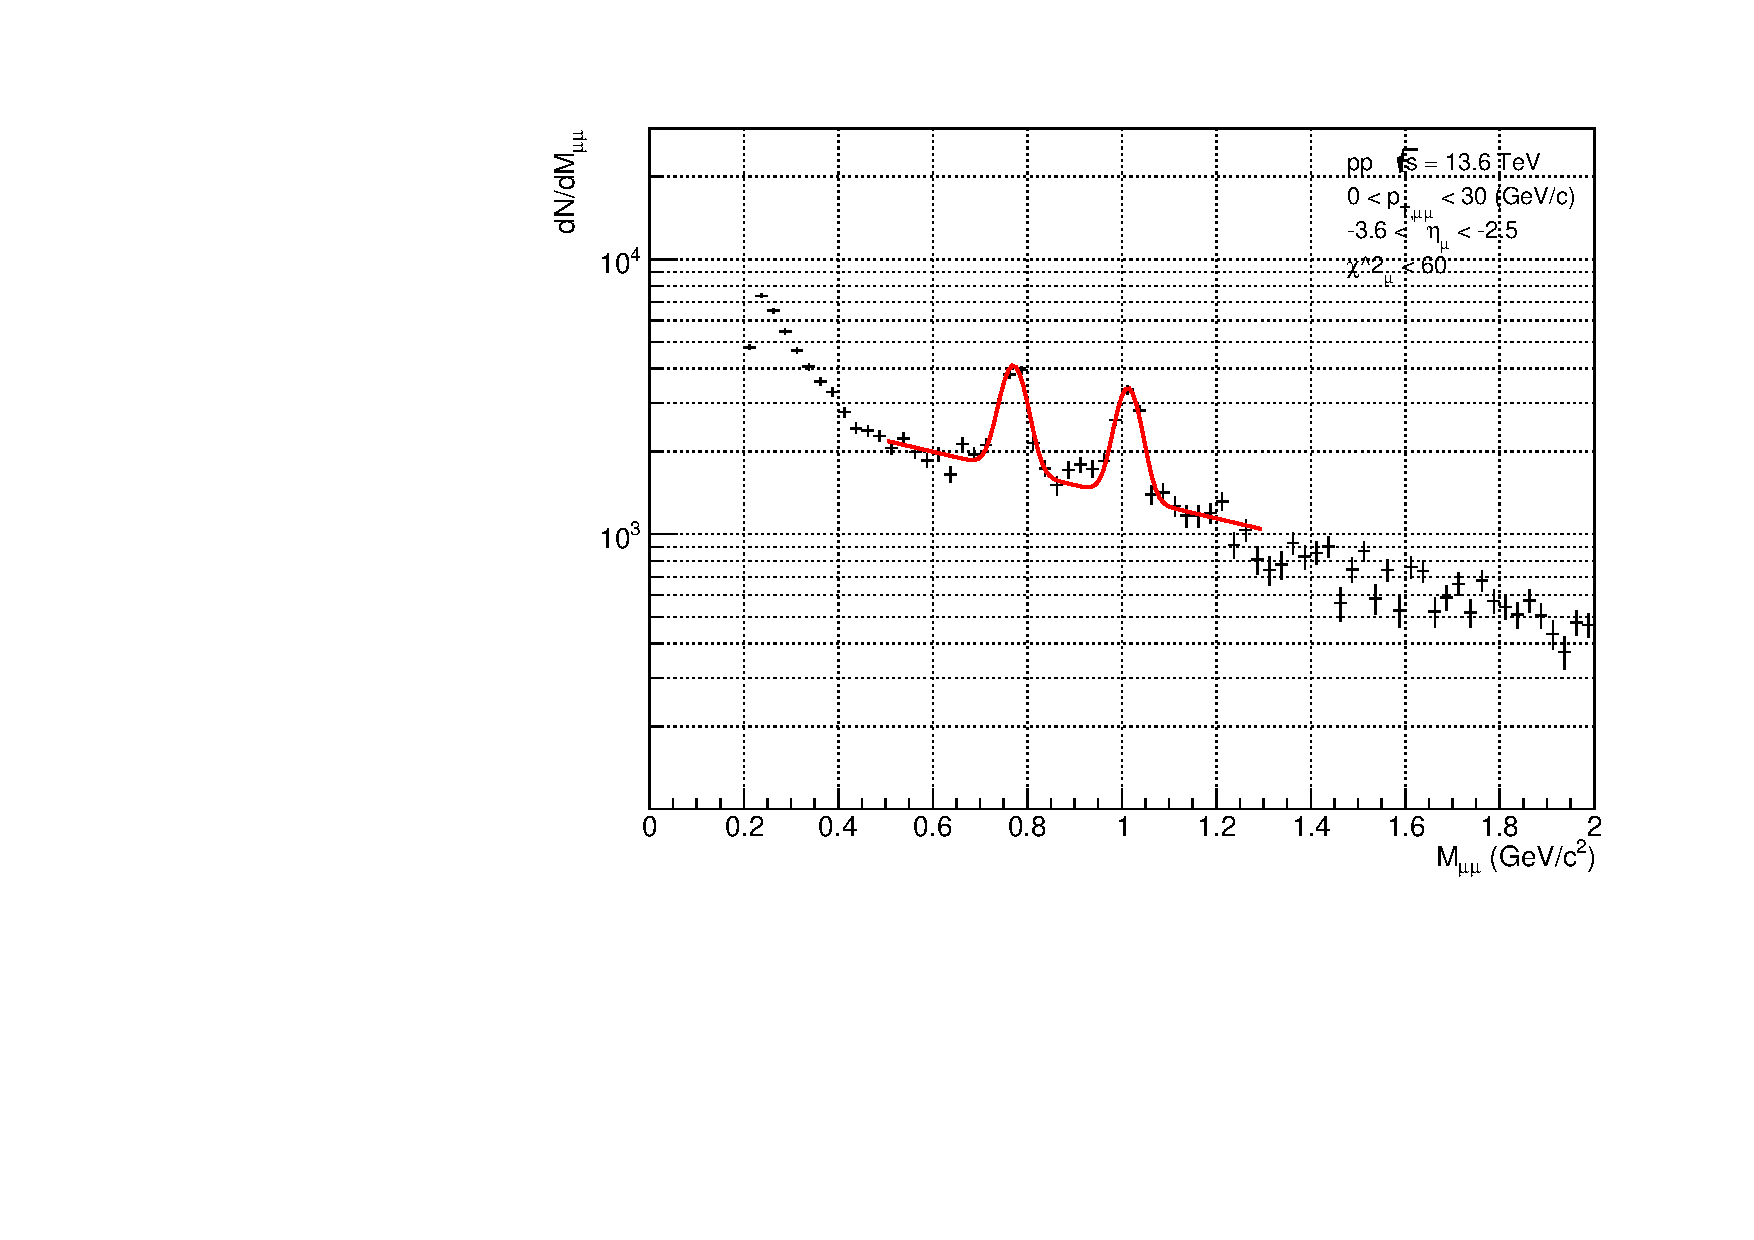
\includegraphics[width=\textwidth]{fig/3_4_4_Fit_chi2_60.pdf}
                    \caption*{MFT-MCH matching $\chi^2 < 60$}
                \end{minipage}
                \hfill
                \begin{minipage}{0.45\textwidth}
                    \centering
                    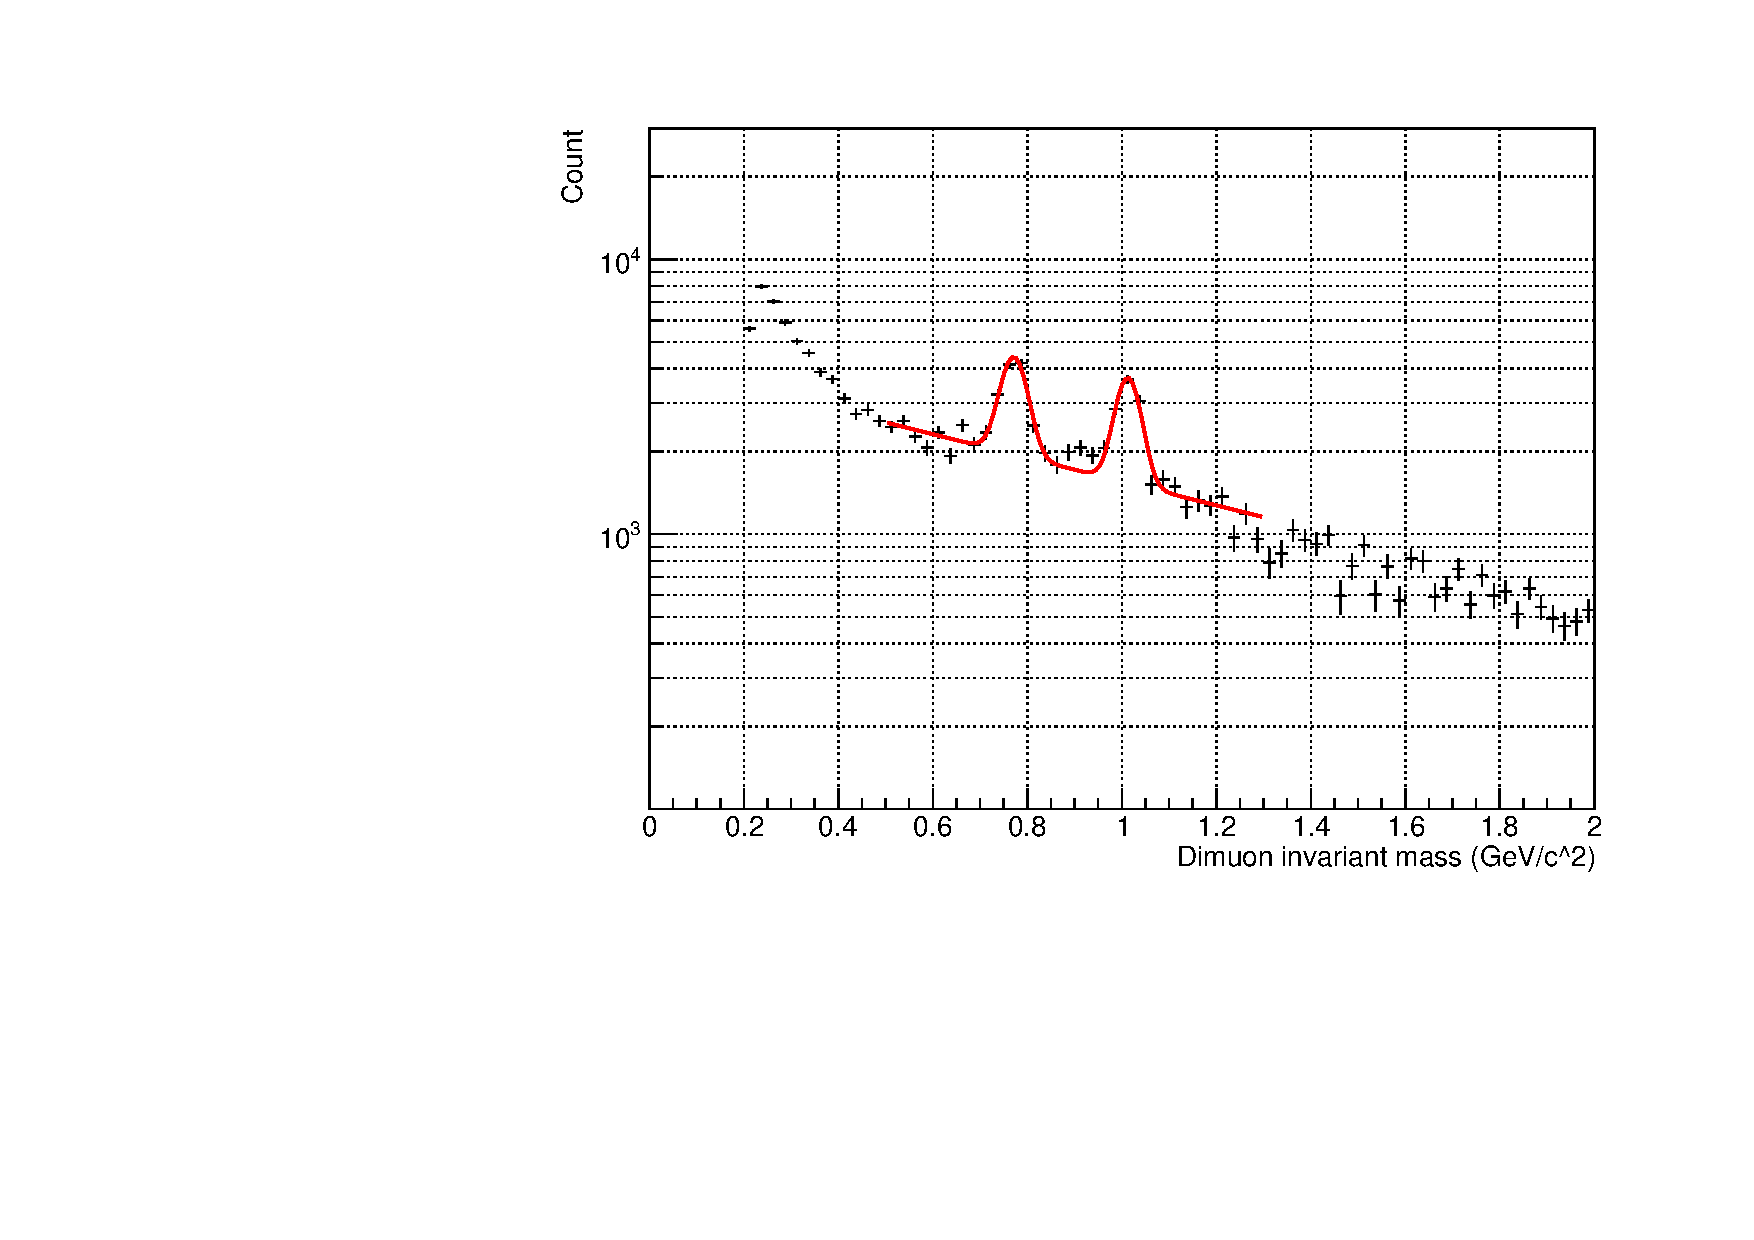
\includegraphics[width=\textwidth]{fig/3_4_4_Fit_chi2_80.pdf}
                    \caption*{MFT-MCH matching $\chi^2 < 80$} 
                \end{minipage}
                \\
                \vspace{1em}
                \begin{minipage}{0.45\textwidth}
                    \centering
                    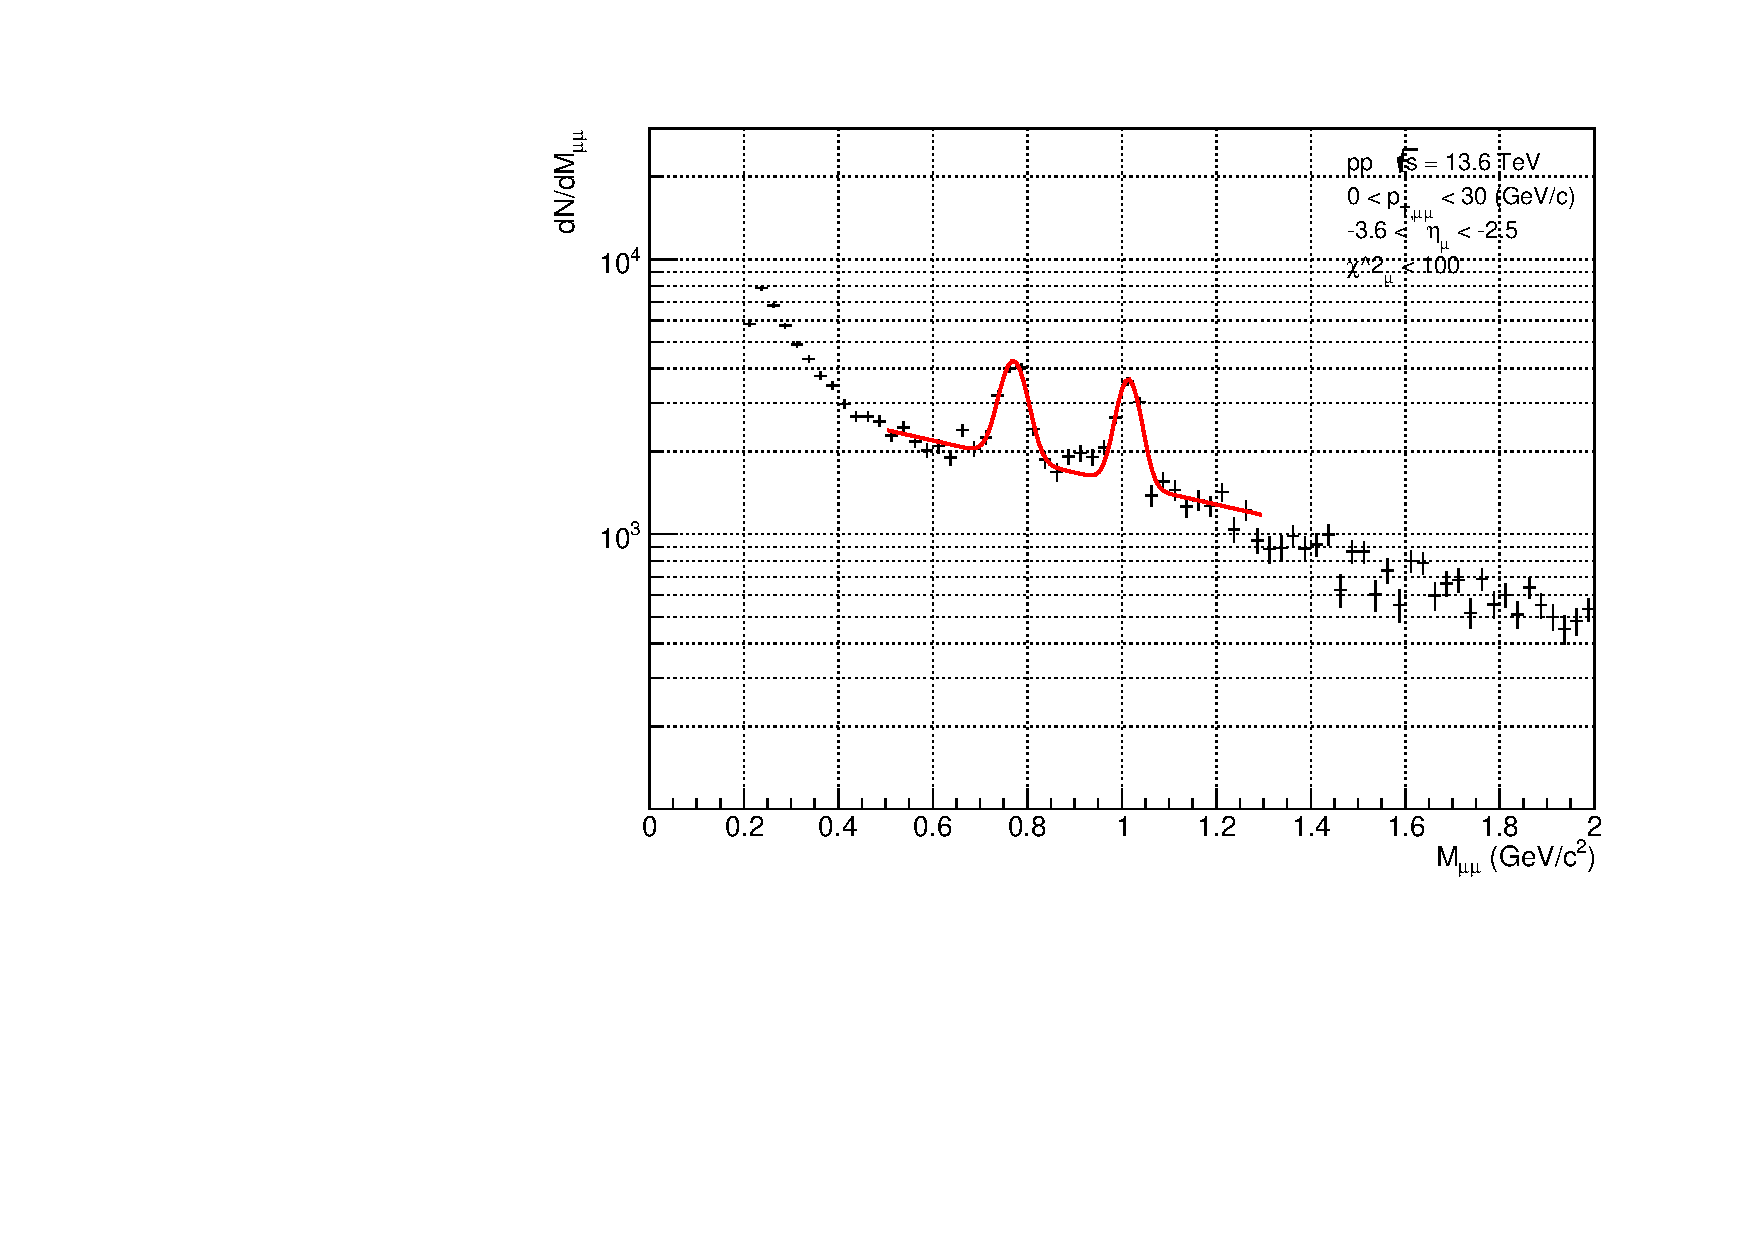
\includegraphics[width=\textwidth]{fig/3_4_4_Fit_chi2_100.pdf}
                    \caption*{MFT-MCH matching $\chi^2 < 100$}
                \end{minipage}
                \hfill
                \begin{minipage}{0.45\textwidth}
                    \centering
                    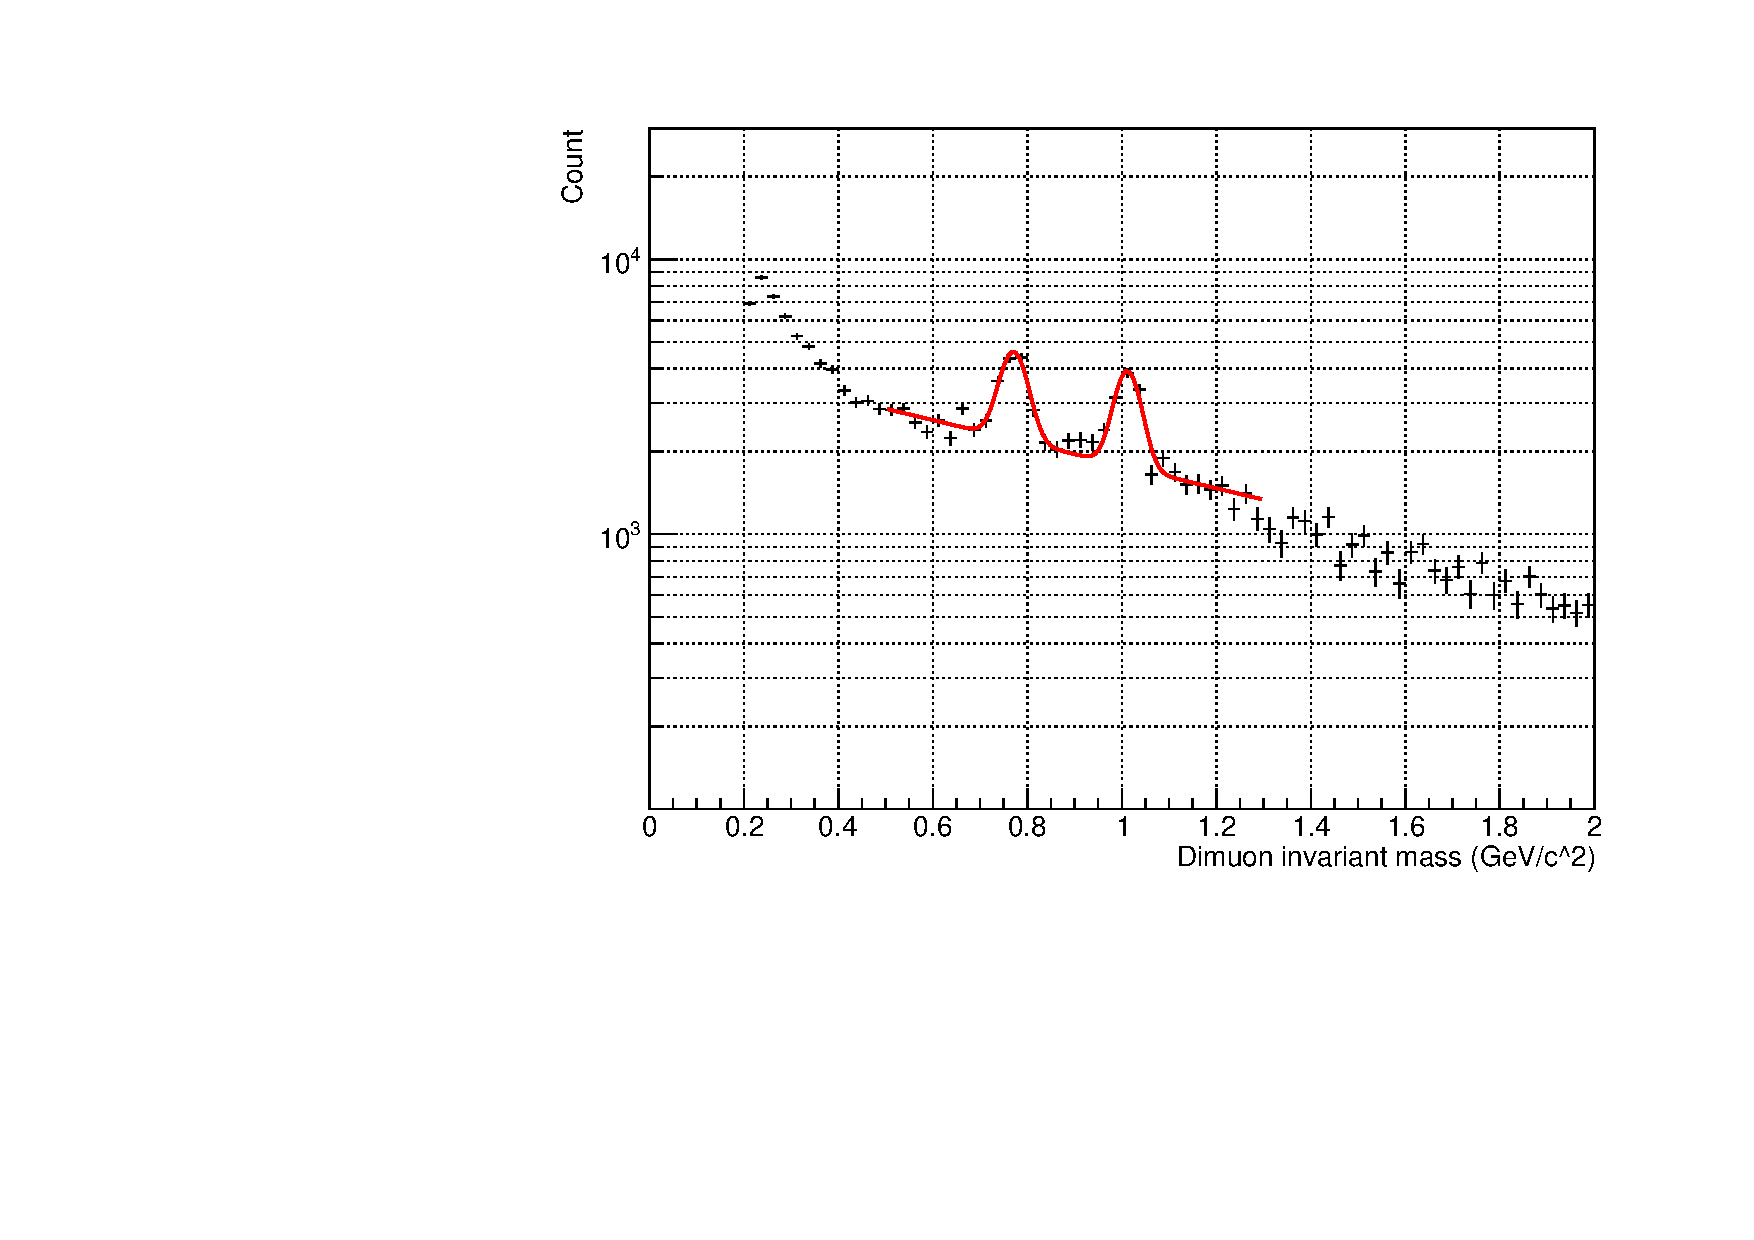
\includegraphics[width=\textwidth]{fig/3_4_4_Fit_chi2_200.pdf}
                    \caption*{MFT-MCH matching $\chi^2 < 200$}
                \end{minipage}
                \caption{MFT-MCH matching $\chi^2$カットを適用した際のピークフィットの結果}
                \label{Analysis:Dimuon:Matching_Fit}
            \end{figure}
            %need addition
            The horizontal axis represents the matching \(\chi^2\), while the vertical axis shows \(S/\sqrt{S+BG}\). As the cut value is reduced, the value of \(S/\sqrt{S+BG}\) increases. When a cut of \(\chi^2<30\) is applied, \(S/\sqrt{S+BG}\) reaches its maximum for both \(\omega\) and \(\phi\).\@ From this result, it is evident that the optimal matching \(\chi^2\) value is \(\chi^2<30\).\@
            \begin{figure}[htbp]
                \centering
                % Left figure
                \begin{minipage}{0.45\textwidth} % minipage for width specification
                    \centering
                    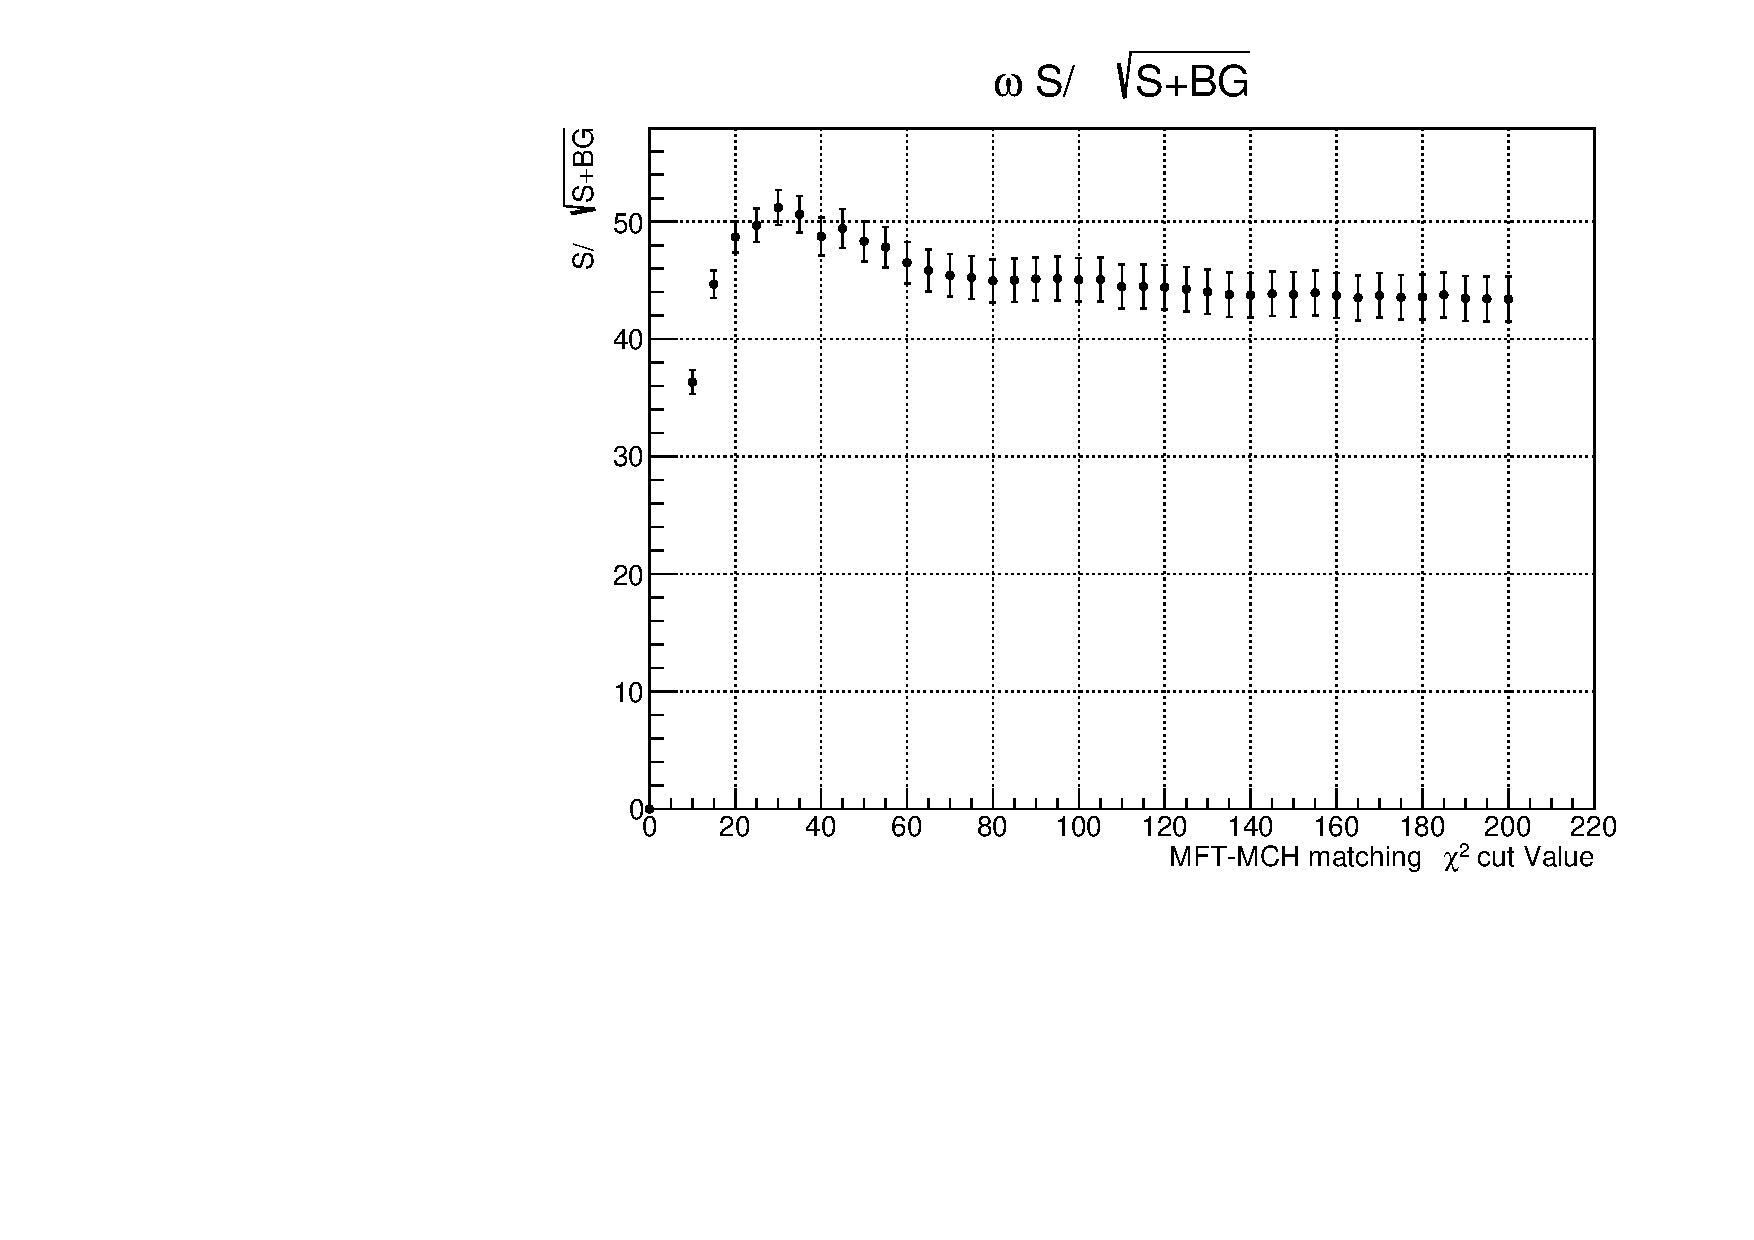
\includegraphics[width=\textwidth]{fig/3_4_4_omega_significance.pdf} % Left image
                    \caption{$\omega$ figure of merit}
                    \label{fig:omega_significance}
                \end{minipage}
                % Right figure
                \hfill
                \begin{minipage}{0.45\textwidth}
                    \centering
                    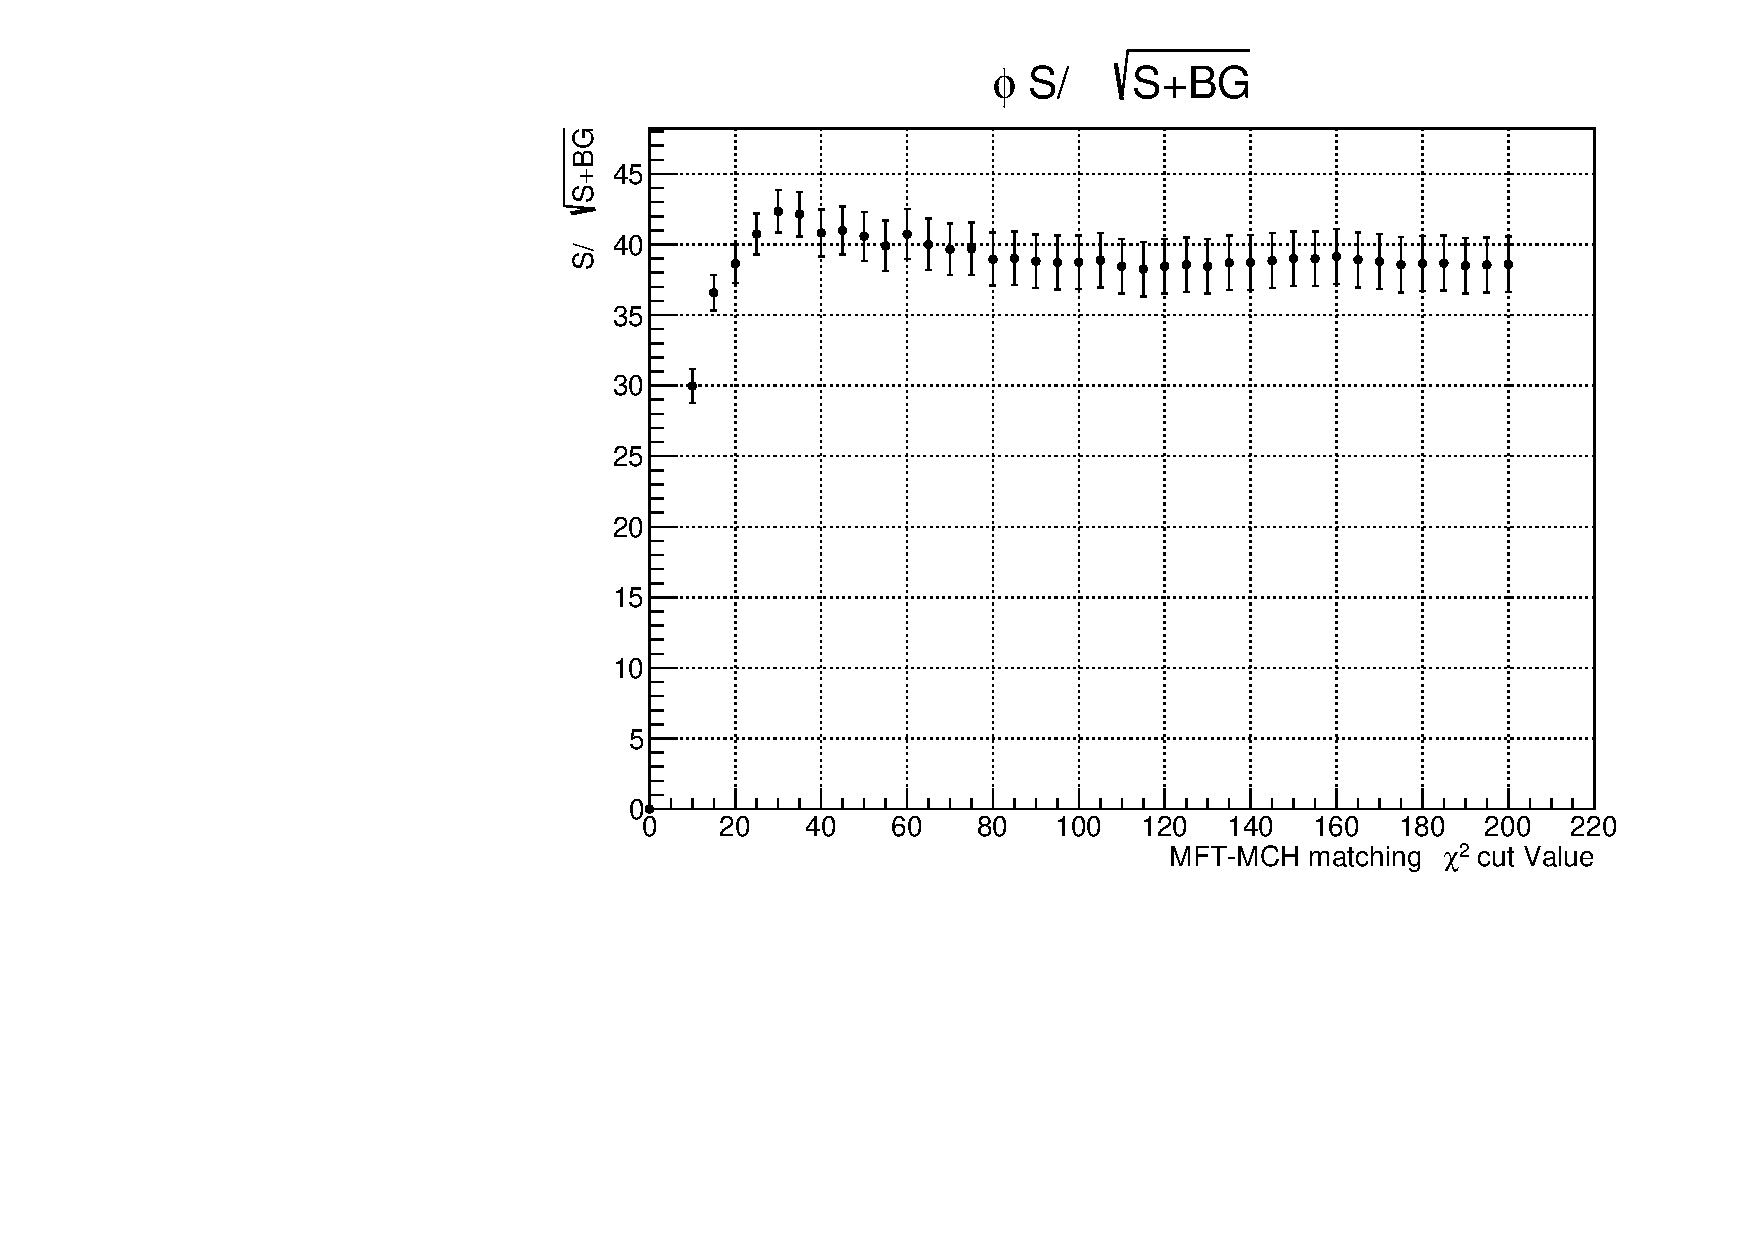
\includegraphics[width=\textwidth]{fig/3_4_4_phi_significance.pdf} % Right image
                    \caption{$\phi$ figure of merit}
                    \label{fig:phi_significance}
                \end{minipage}
            \end{figure}

        \subsubsection{Fake Match Track Removal Analysis of MFT-MCH-MID Track using MFT Track $\eta$ - MCH Track $\eta$}
        \label{Analysis:Matching}
            The \(\eta\) distribution of Global Tracks differs significantly from the true distribution. This discrepancy arises due to muon reconstruction involving the MFT, indicating issues with MFT-MCH matching. Fake matches contribute to this significantly distorted \(\eta\) distribution. By removing these distortions, it is shown that the resolution of \(\eta\), \(p_T\), and \(\phi\) for single muons improves. In this analysis, Fake matches are removed by utilizing the difference in \(\eta\) between the MFT Track and MCH Track that constitute the Global Track. The dataset used is LHC24b1, which consists of Monte Carlo data of \(pp\) collisions at \(\sqrt{s} = 13.6\) TeV from minimum-bias events. This simulation data has been compared with real data, confirming that they exhibit the same behavior. %\ref{Appendix:compair_Real_and_MC}
            \begin{figure}[H]
                \centering
                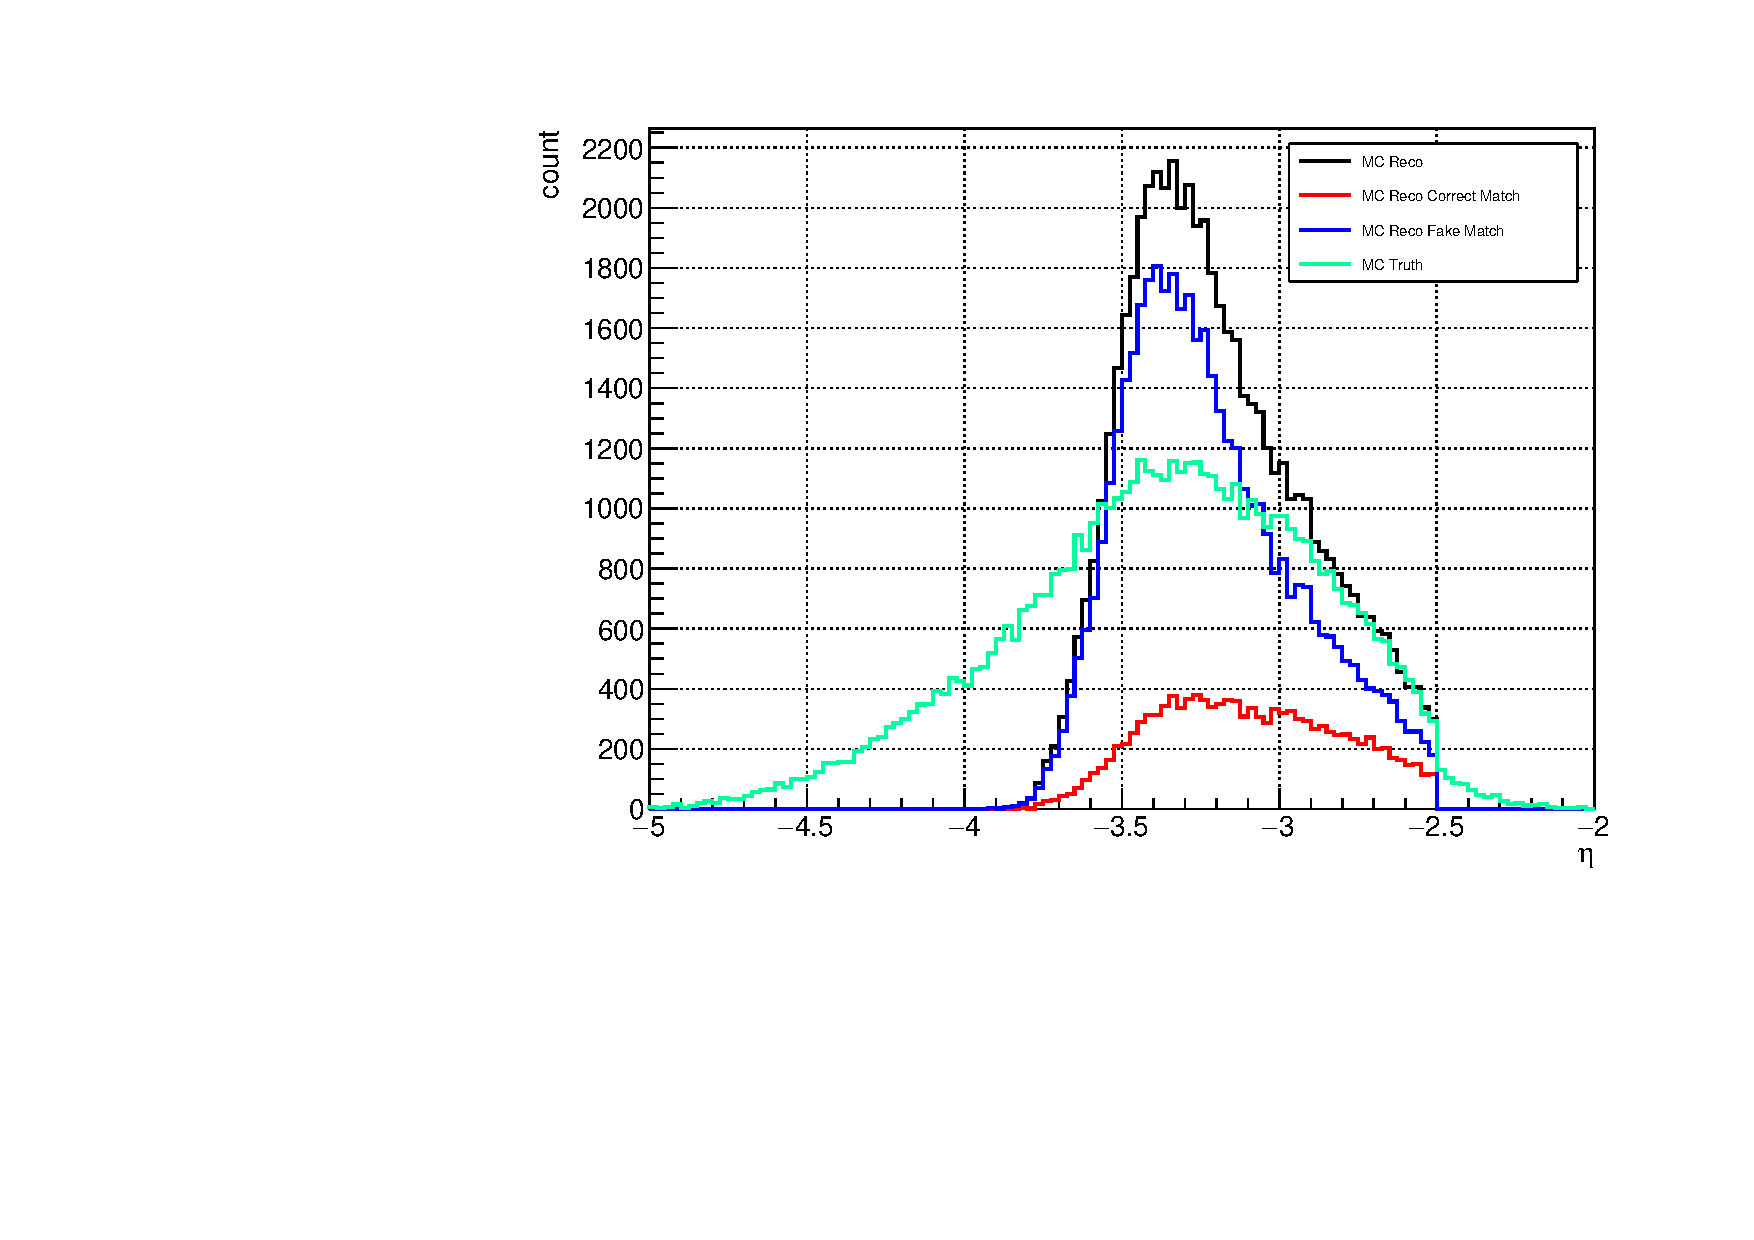
\includegraphics[keepaspectratio, scale=0.5]{fig/3_5_6_etacutno_eta.pdf}
                \caption{$\eta$ distribution of Global Track}
                \label{Analysis:Matching:eta}
            \end{figure}
            Figure \ref{Analysis:Matching:eta} shows the \(\eta\) distribution of Global Tracks for all \(p_T\) regions. The black histogram represents the reconstructed \(\eta\) distribution of Global Tracks. The blue histogram corresponds to the \(\eta\) distribution of reconstructed tracks identified as Fake matches, while the red histogram represents the \(\eta\) distribution of correctly matched tracks. The green histogram represents the true \(\eta\) distribution corresponding to the black reconstructed tracks.  
            Comparing the black reconstructed muon distribution with the green true distribution, the acceptance range of MFT-MCH-MID Tracks is \(-3.6 < \eta < -2.5\). However, in the green distribution, muons with \(\eta\) values smaller than \(-3.6\) are reconstructed within the \(-3.6 < \eta < -2.5\) range. This phenomenon is likely caused by muons that passed through the absorber and subsequently traversed the MCH-MID system while being outside the MFT acceptance. 
            To remove such tracks, a \(\Delta \eta\) cut is applied as (\ref{Deltaeta_eq}).
            \begin{eqnarray}
                \label{Deltaeta_eq}
                \Delta \eta = \text{MFT} \, \eta - \text{MCH} \, \eta  
            \end{eqnarray}
            For each track, \(\Delta \eta\) was calculated. Fig.\ref{Analysis:Matching:DeltaEta} shows the distribution. The black represents the distribution of reconstructed muons, the blue represents the distribution of Fake Match tracks, and the red represents the distribution of Correct Match tracks.
            \begin{figure}[H]
                \centering
                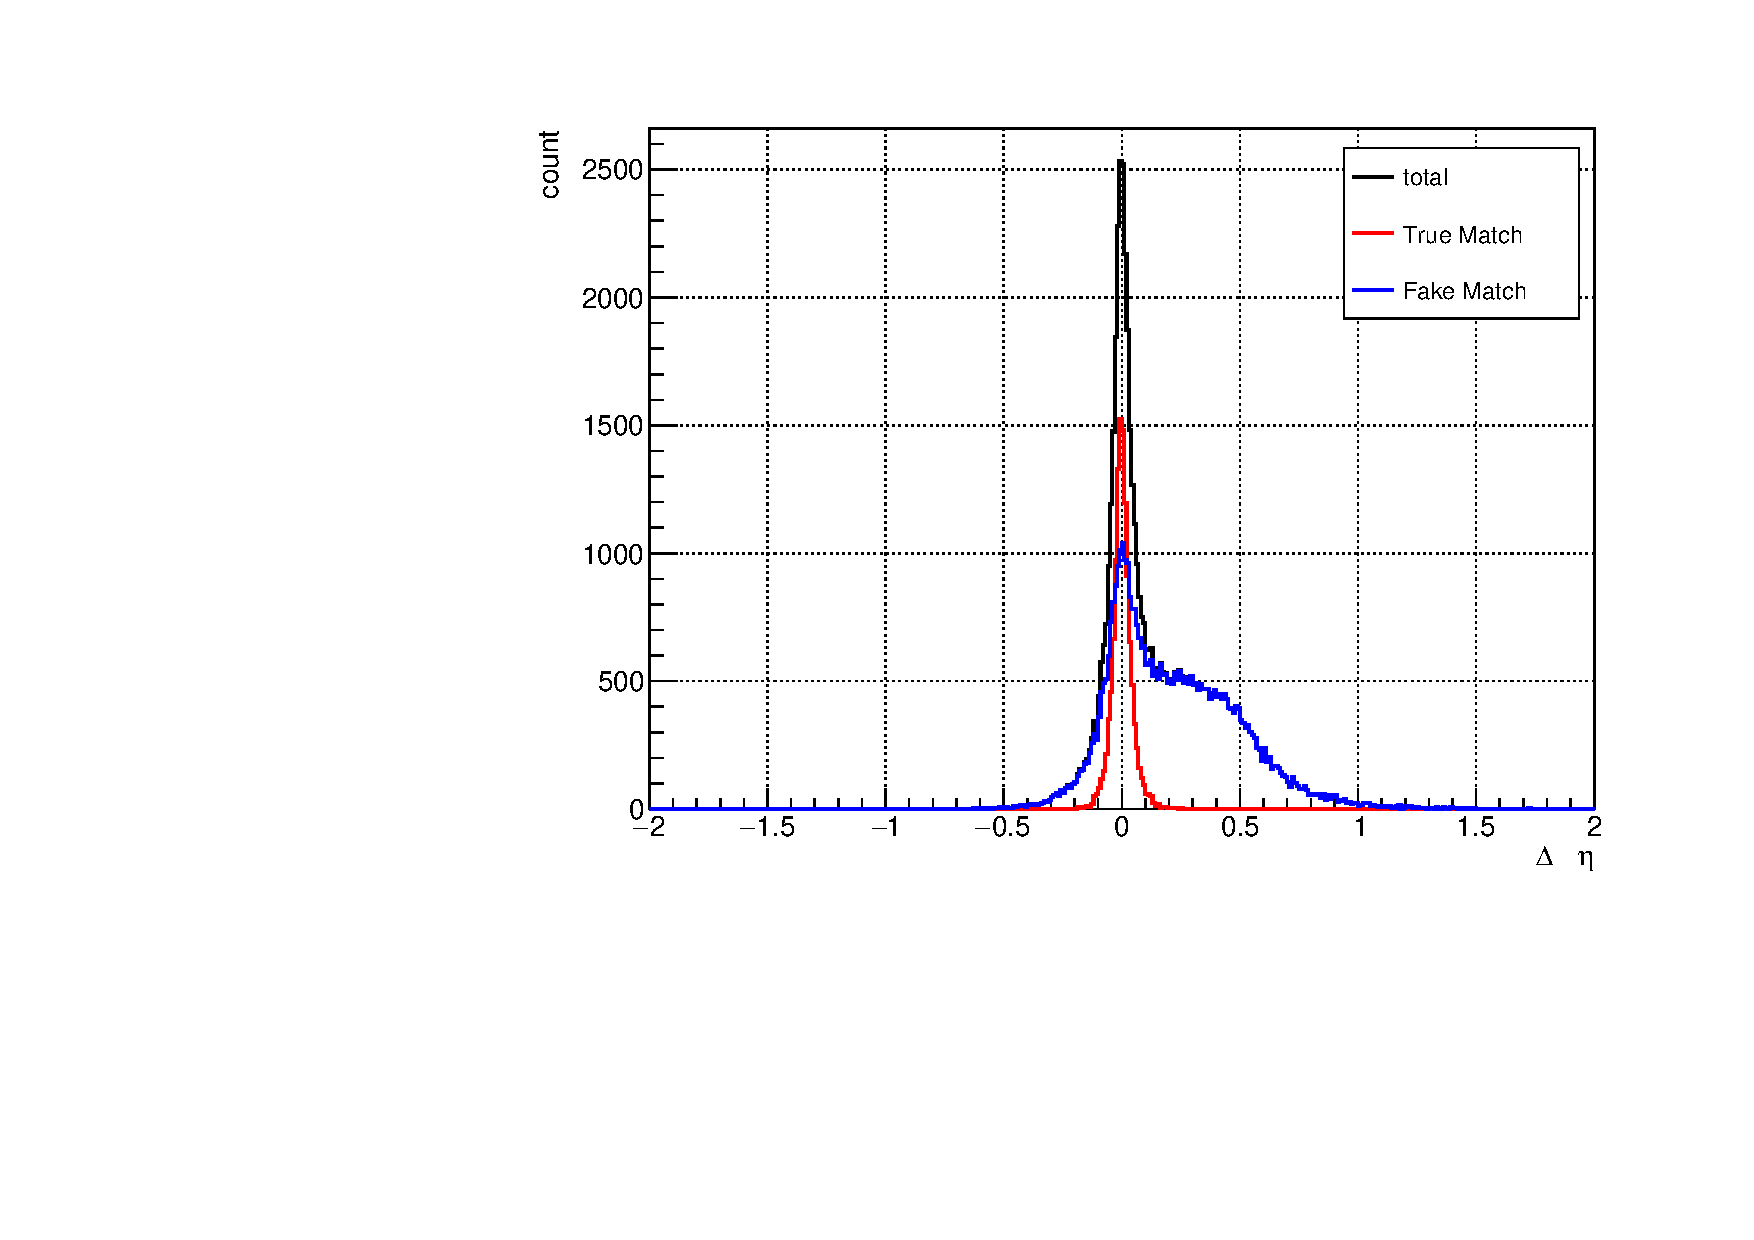
\includegraphics[keepaspectratio, scale=0.5]{fig/3_5_6_etacutno_deltaeta.pdf} % 右側の画像
                \caption{$\Delta \eta$ distribution}
                \label{Analysis:Matching:DeltaEta}
            \end{figure}
            For \( |\Delta \eta| > 0.2 \), Fake Match tracks dominate. By applying a \( |\Delta \eta| < 0.2 \) cut to remove Fake Matches while retaining as many Correct Matches as possible, the distributions and resolutions of each physical quantity are shown for this case.
            \begin{figure}[H]
                \centering
                % 左側の図
                \begin{minipage}{0.45\textwidth} % minipage で横幅を指定
                    \centering
                    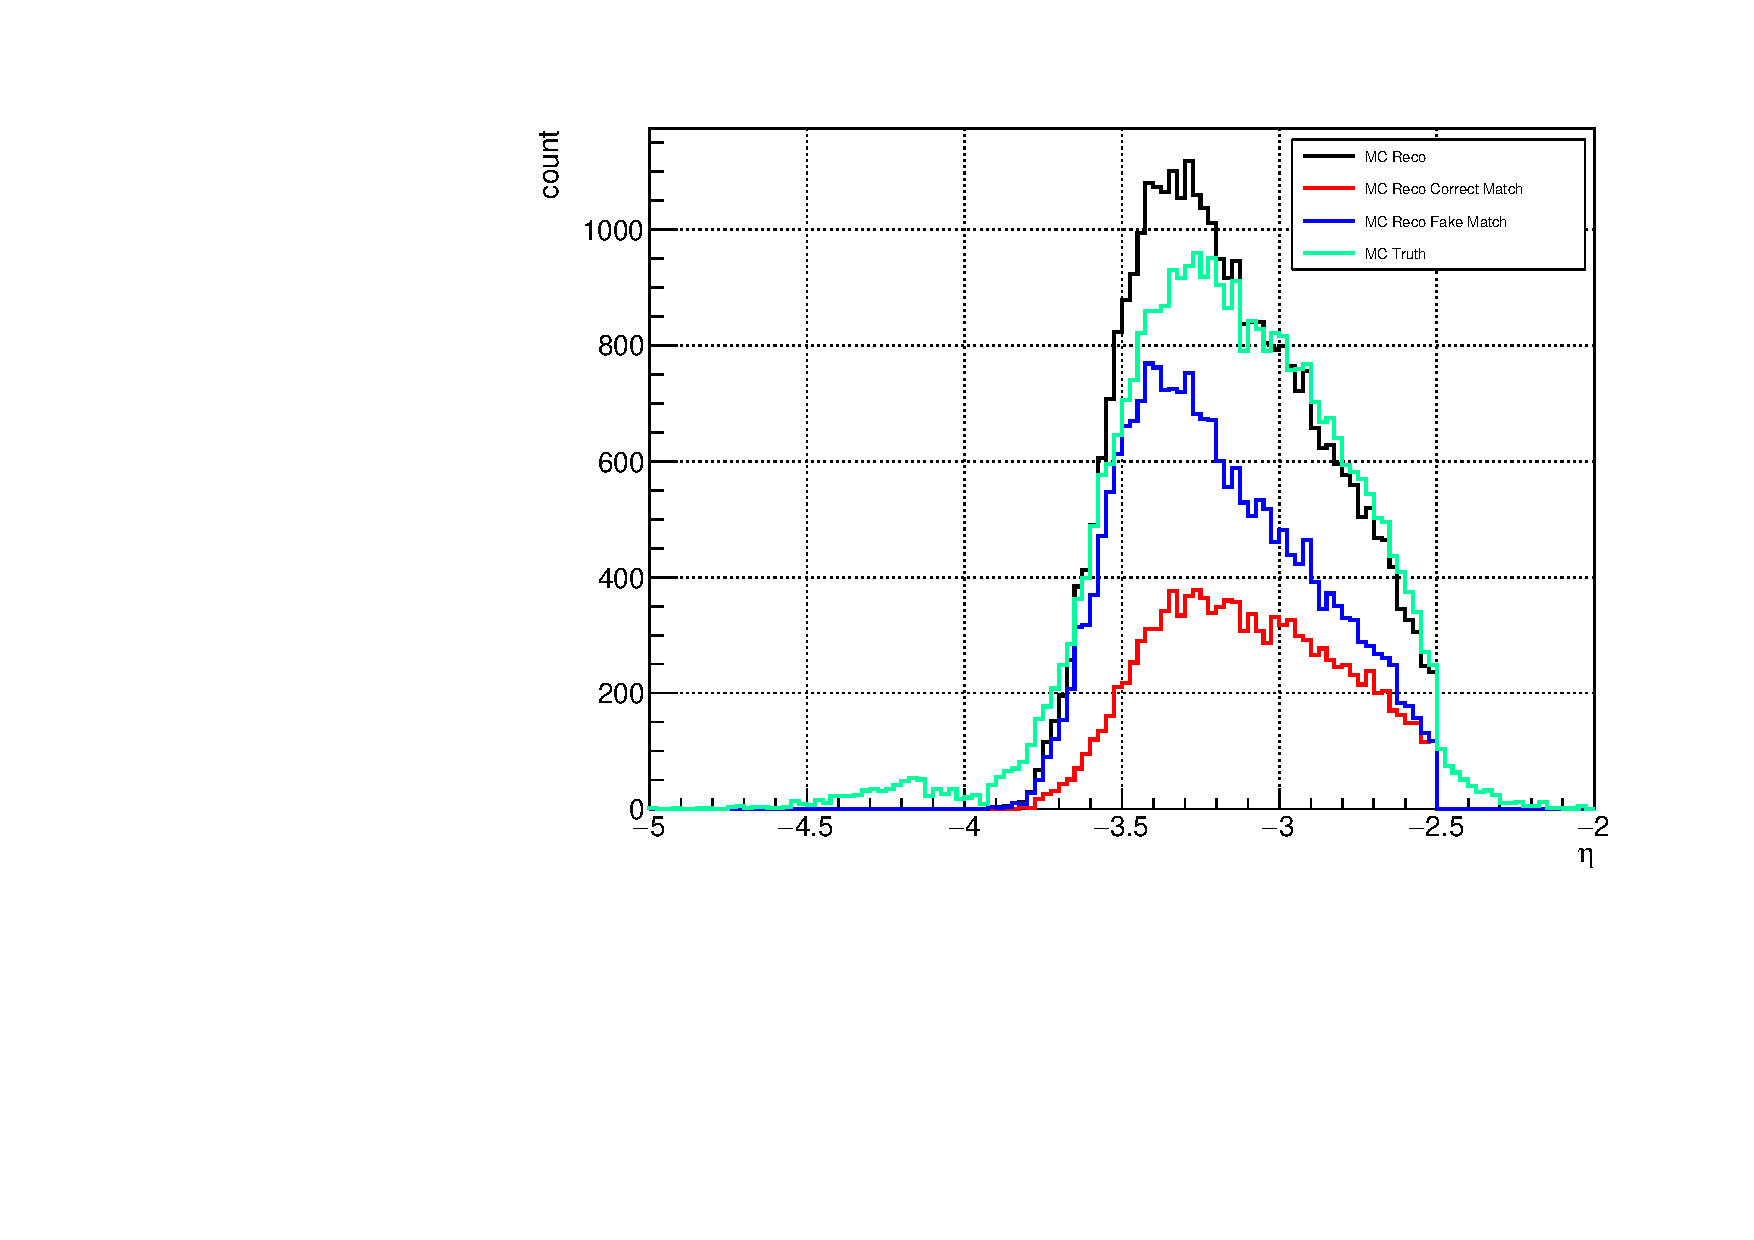
\includegraphics[width=\textwidth]{fig/3_5_6_etacut02_eta.pdf} % 左側の画像
                    \caption{The $\eta$ distribution of Global Tracks after the $\Delta \eta$ cut}
                    \label{Analysis:Matching:afterCut_eta}
                \end{minipage}
                % 右側の図
                \hfill
                \begin{minipage}{0.45\textwidth}
                    \centering
                    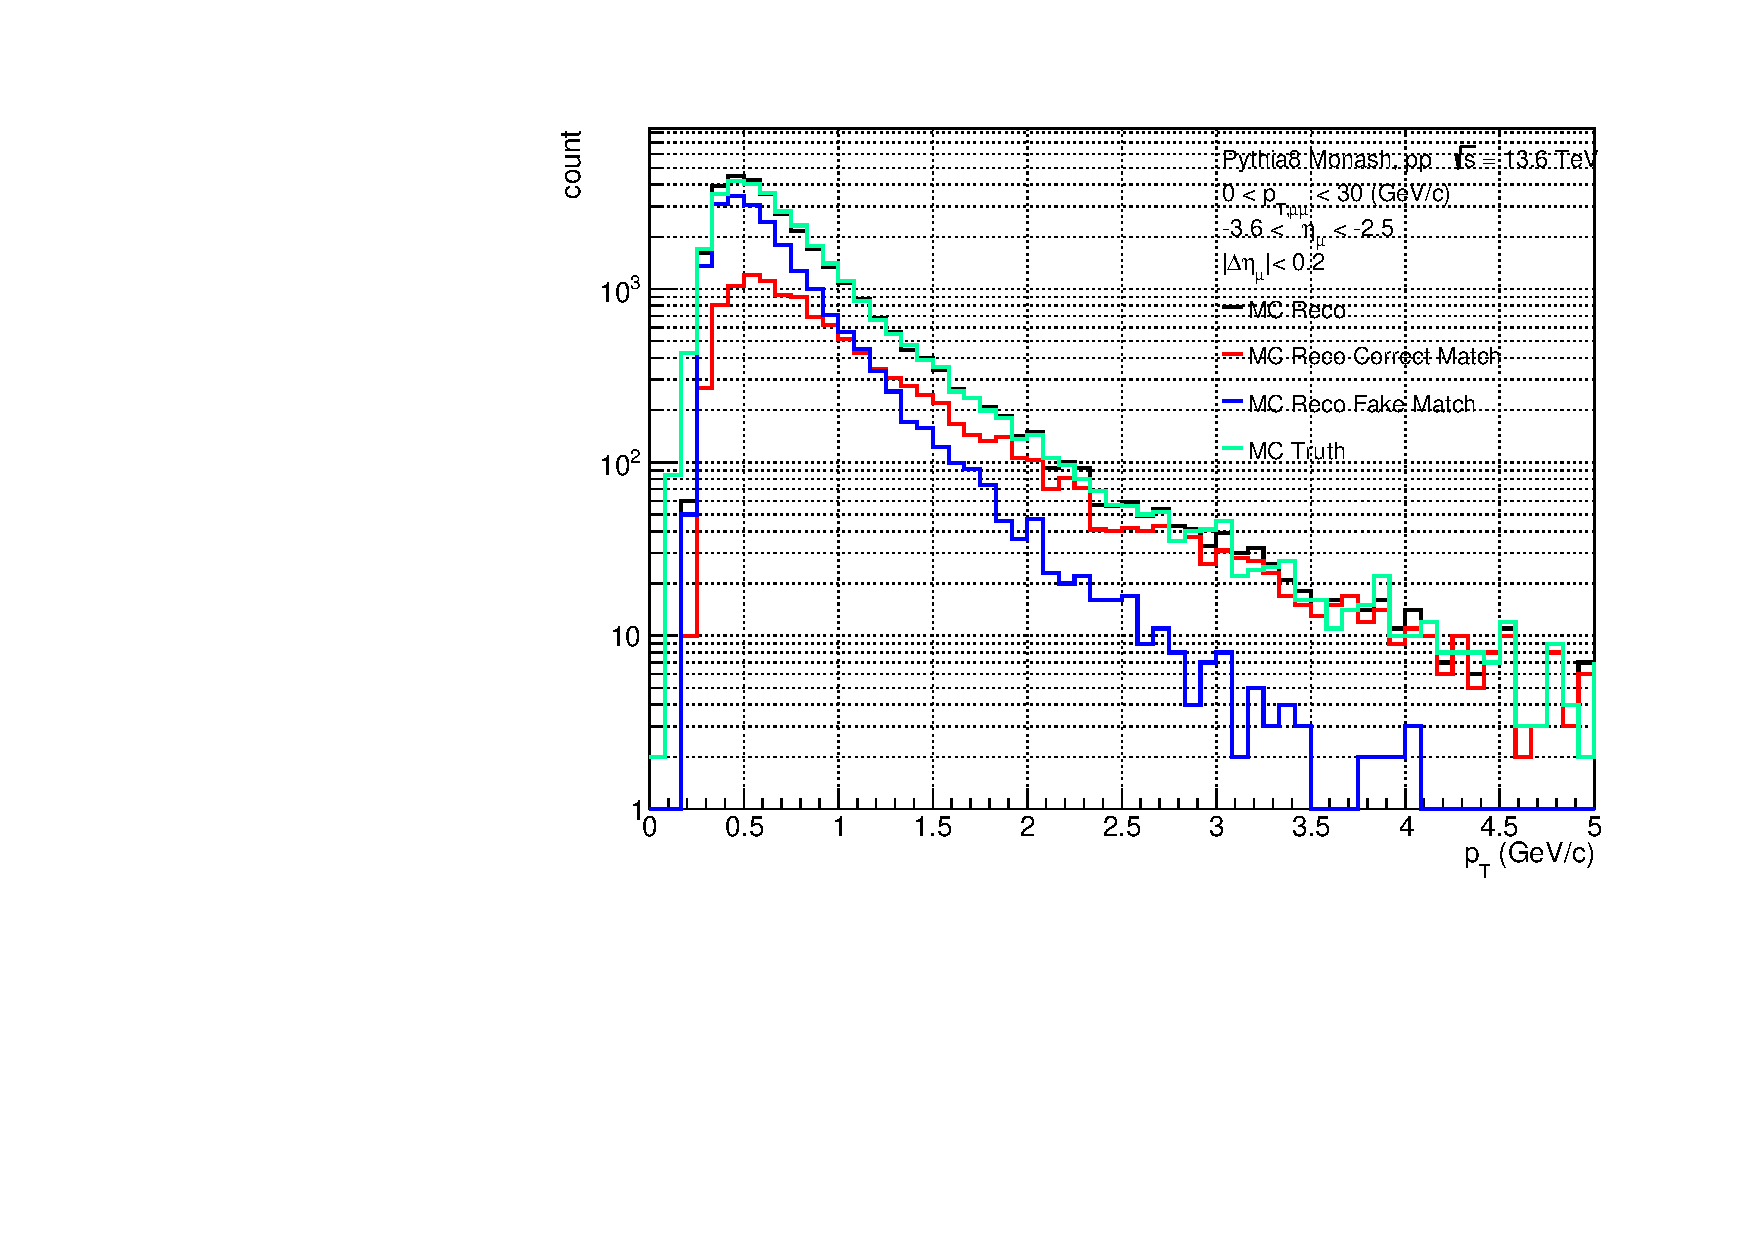
\includegraphics[width=\textwidth]{fig/3_5_6_etacut02_pt.pdf} % 右側の画像
                    \caption{The $p_T$ distribution of Global Tracks after the $\Delta \eta$ cut}
                    \label{Analysis:Matching:afterCut_pt}
                \end{minipage}-
            \end{figure}
            Fig.\ref{Analysis:Matching:afterCut_eta} shows the \(\eta\) distribution after the \(\Delta \eta\) cut. Additionally, Fig.\ref{Analysis:Matching:afterCut_pt} displays the \(p_T\) distribution after the \(\Delta \eta\) cut. As in Figure \ref{Analysis:Matching:eta}, the black histogram represents all reconstructed muon tracks, the red represents Correct match tracks, and the blue represents Fake Match tracks. The green histogram corresponds to the true \(\eta\) distribution for the black muons. Comparing the green distribution of \(\eta\) after the cut with Figure \ref{Analysis:Matching:eta}, we see that the muons distributed at \(\eta < -3.8\) have been removed. Furthermore, this cut successfully removes a large portion of the Fake match tracks that were present in the range of \(-3.6 < \eta < -3.2\). However, as can be seen from Figure \ref{Analysis:Matching:afterCut_pt}, Fake matches originating from low transverse momentum still remain.
            \begin{figure}[H]
                \centering
                    \begin{minipage}{0.45\textwidth}
                        \centering
                        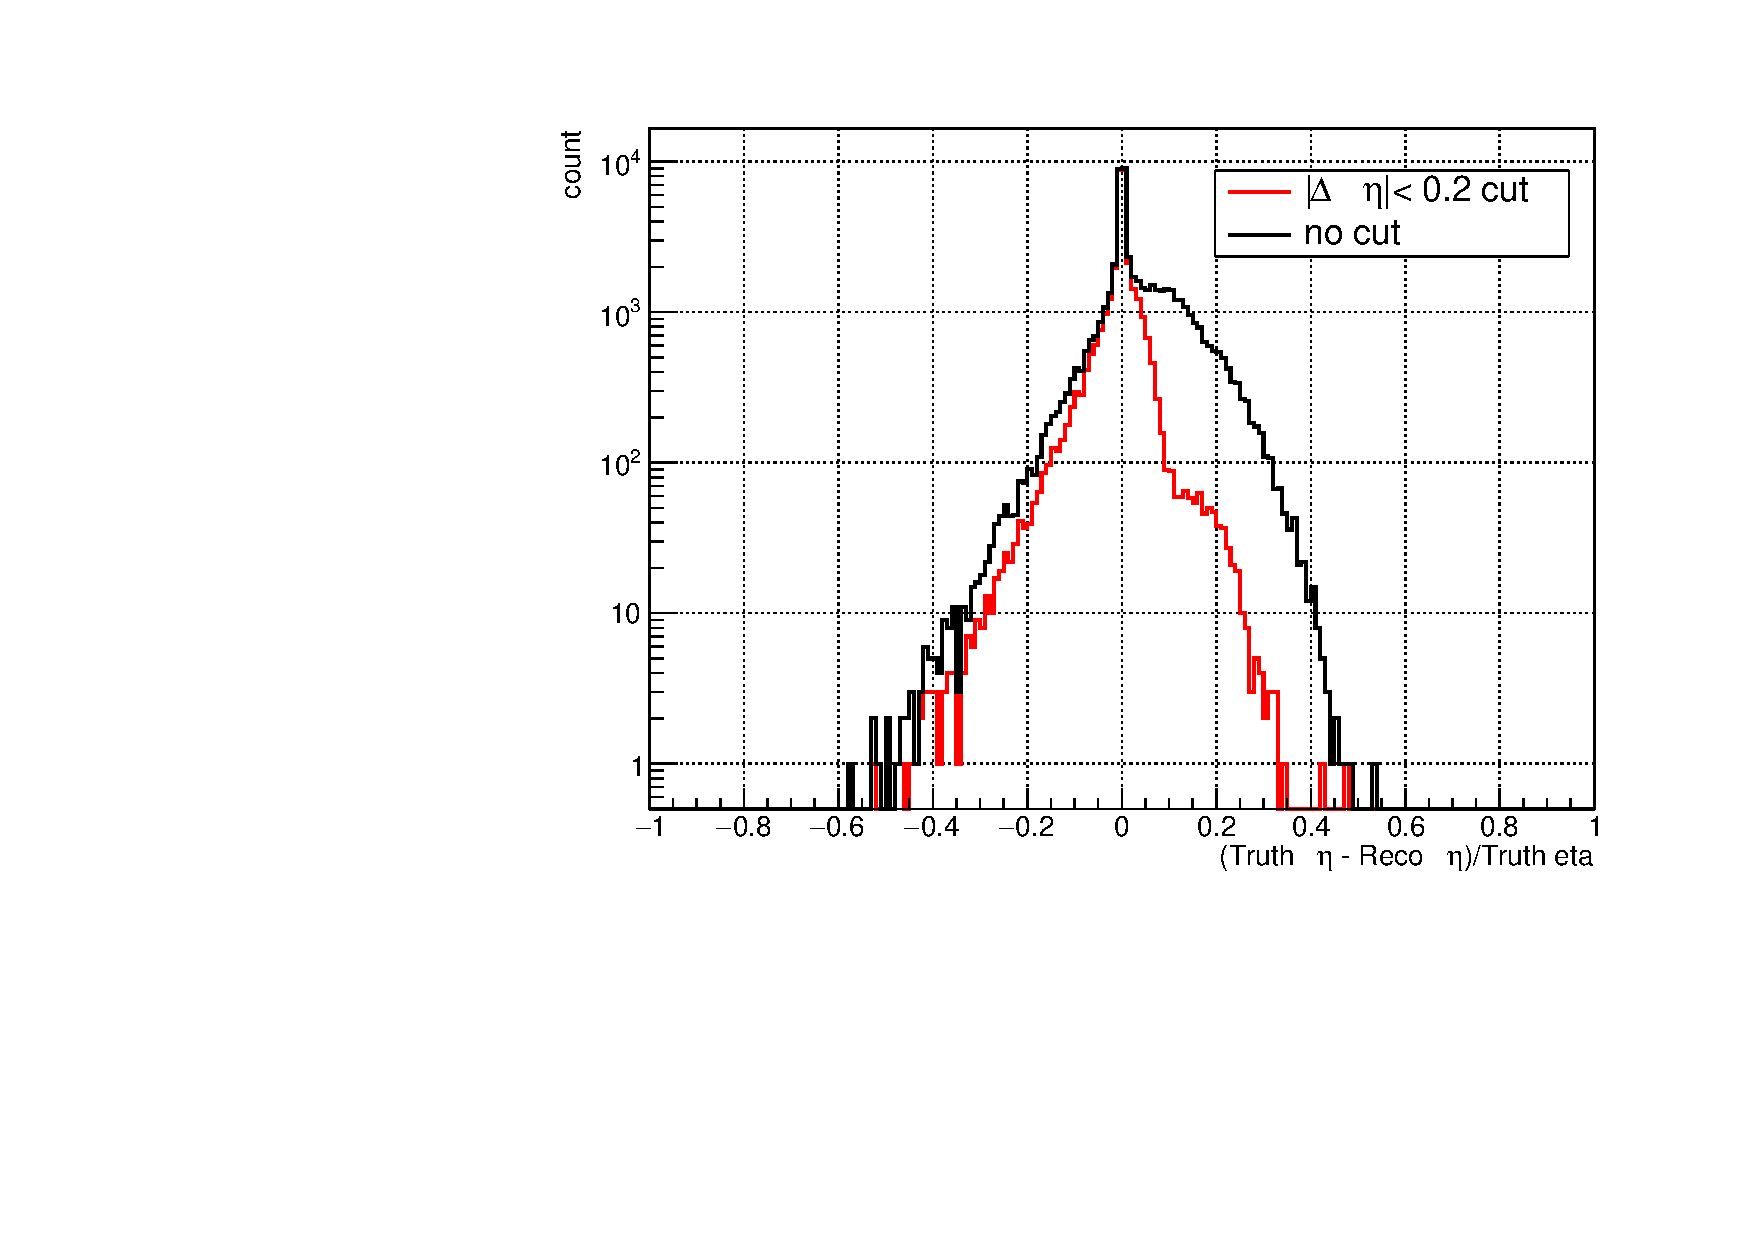
\includegraphics[width=\textwidth]{fig/3_5_6_reso_eta.pdf} 
                        \caption{Resolution of $\eta$}
                        \label{Analysis:Matching:pt resolution}
                    \end{minipage}
                    \begin{minipage}{0.45\textwidth}
                        \centering
                        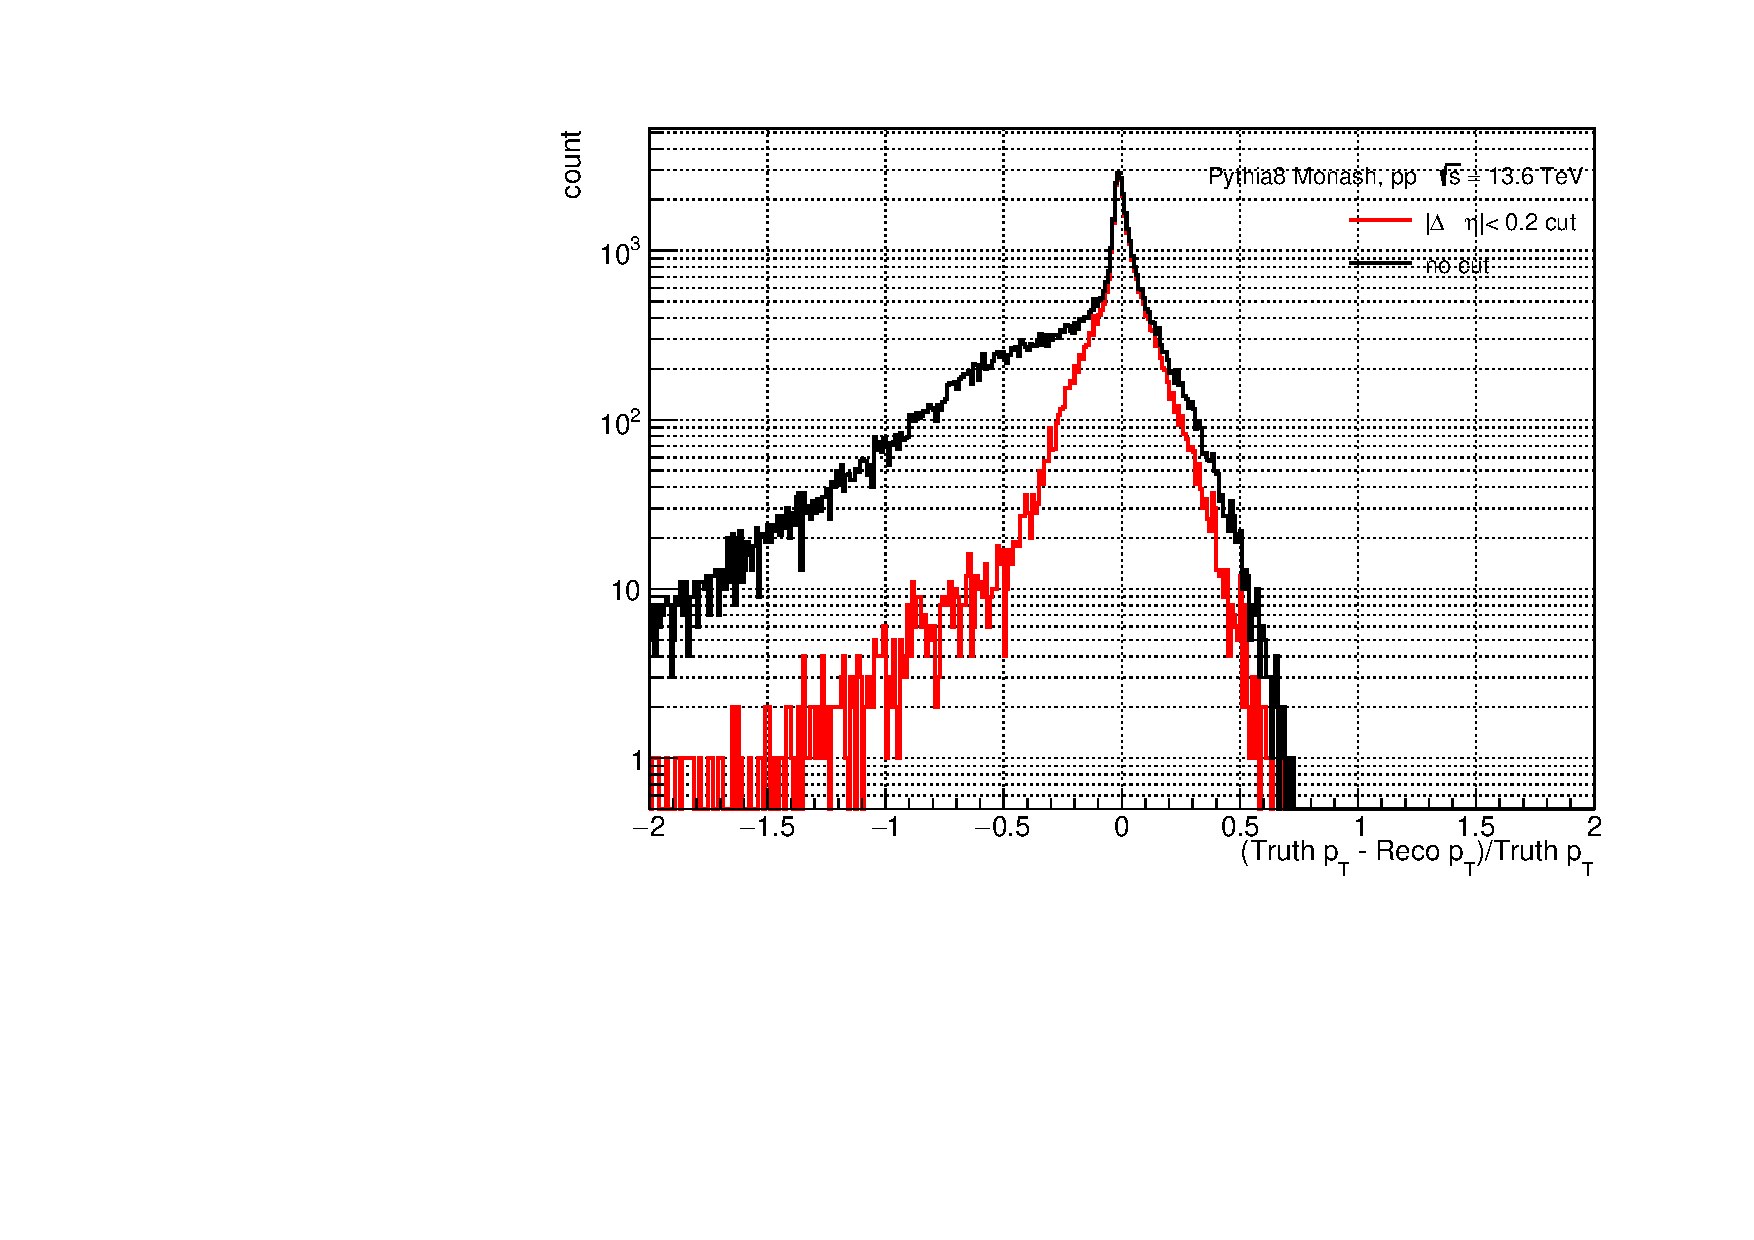
\includegraphics[width=\textwidth]{fig/3_5_6_reso_pt.pdf} 
                        \caption{Resolution of $p_T$}
                        \label{Analysis:Matching:eta resolution}
                    \end{minipage}
                \end{figure}
                \begin{figure}[H]
                    \centering
                    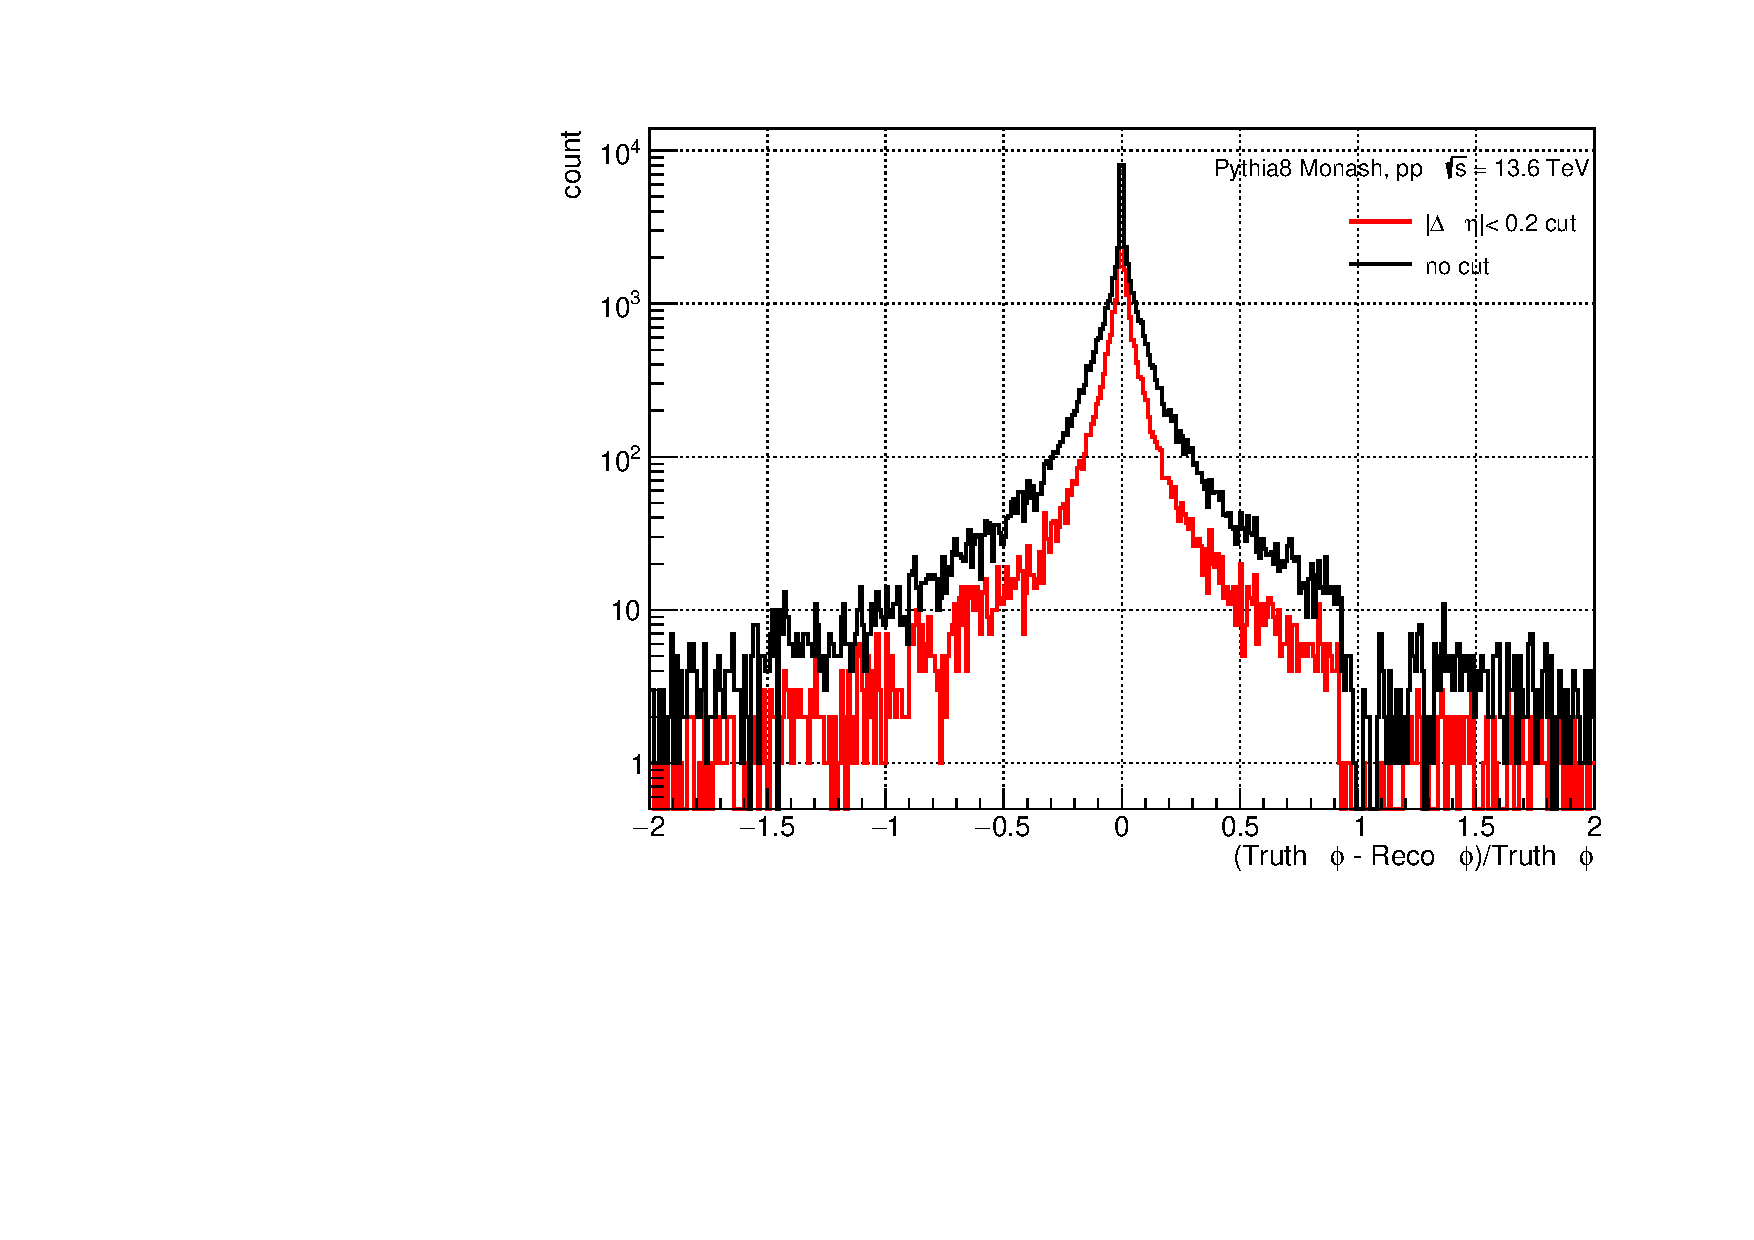
\includegraphics[keepaspectratio, scale=0.4]{fig/3_5_6_reso_phi.pdf} 
                    \caption{Resolution of $\phi$}
                    \label{Analysis:Matching:phi resolution}
                \end{figure}
            Figures \ref{Analysis:Matching:pt resolution}, \ref{Analysis:Matching:eta resolution}, and \ref{Analysis:Matching:phi resolution} show the resolution of \(p_T\), \(\eta\), and \(\phi\), respectively. The horizontal axis represents the resolution, which is calculated by subtracting the reconstructed quantity from the true physical quantity and then dividing by the true value. The vertical axis represents the count. The black distribution shows the resolution without applying the \(\Delta \eta\) cut, while the red distribution shows the tracks after applying the \(|\Delta \eta| < 0.2\) cut. By comparing the black and red histograms, it is clear that the resolution has small value for all distributions. This shows that the resolution improves with the cut. Next, we will describe the efficiency and matching purity improvements due to the cut.
            \begin{figure}[htbp]
                \centering
                \begin{minipage}{0.45\textwidth}
                    \centering
                    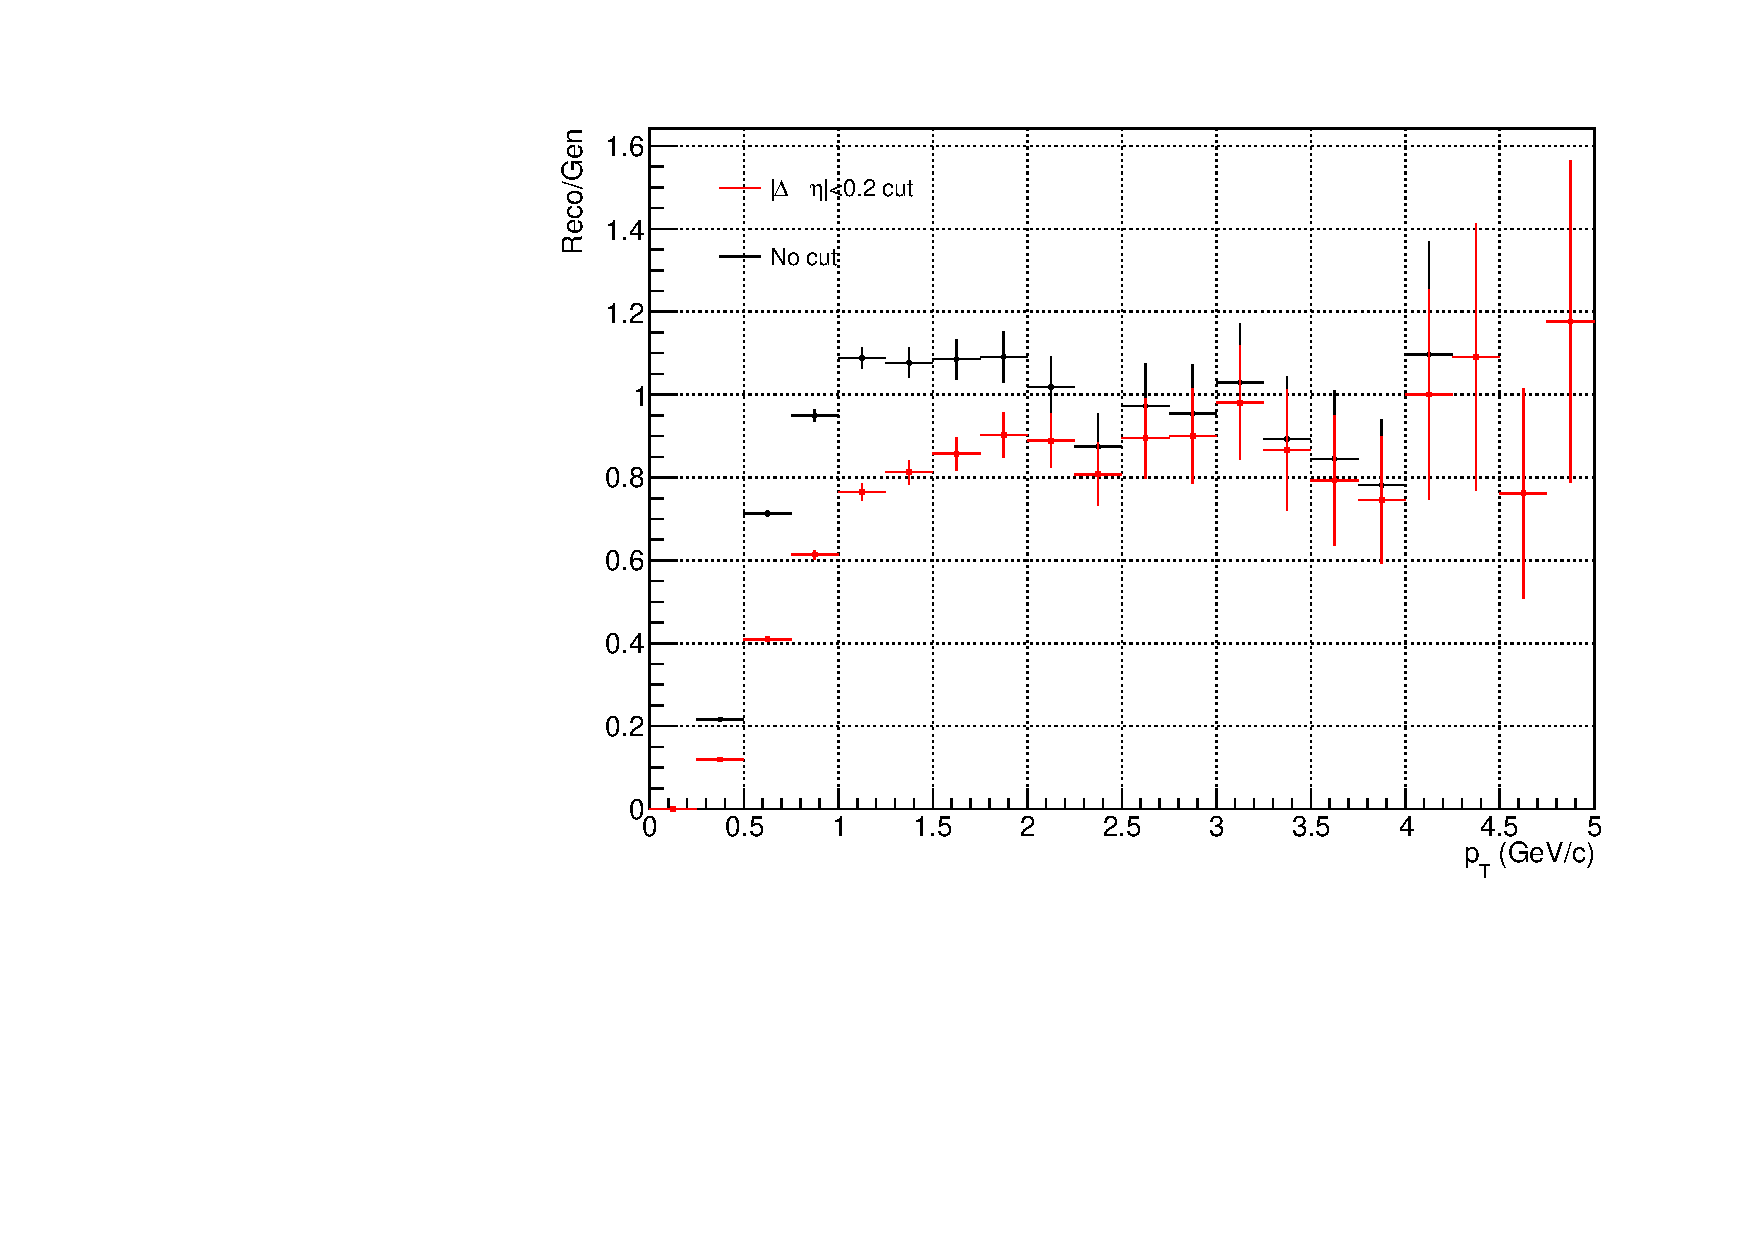
\includegraphics[width=\textwidth]{fig/3_5_6_efficiency_pt.pdf}
                    \captionsetup{labelformat=empty}
                    \caption{Efficency of $p_T$}
                \end{minipage}
                \hfill
                \begin{minipage}{0.45\textwidth}
                \centering
                    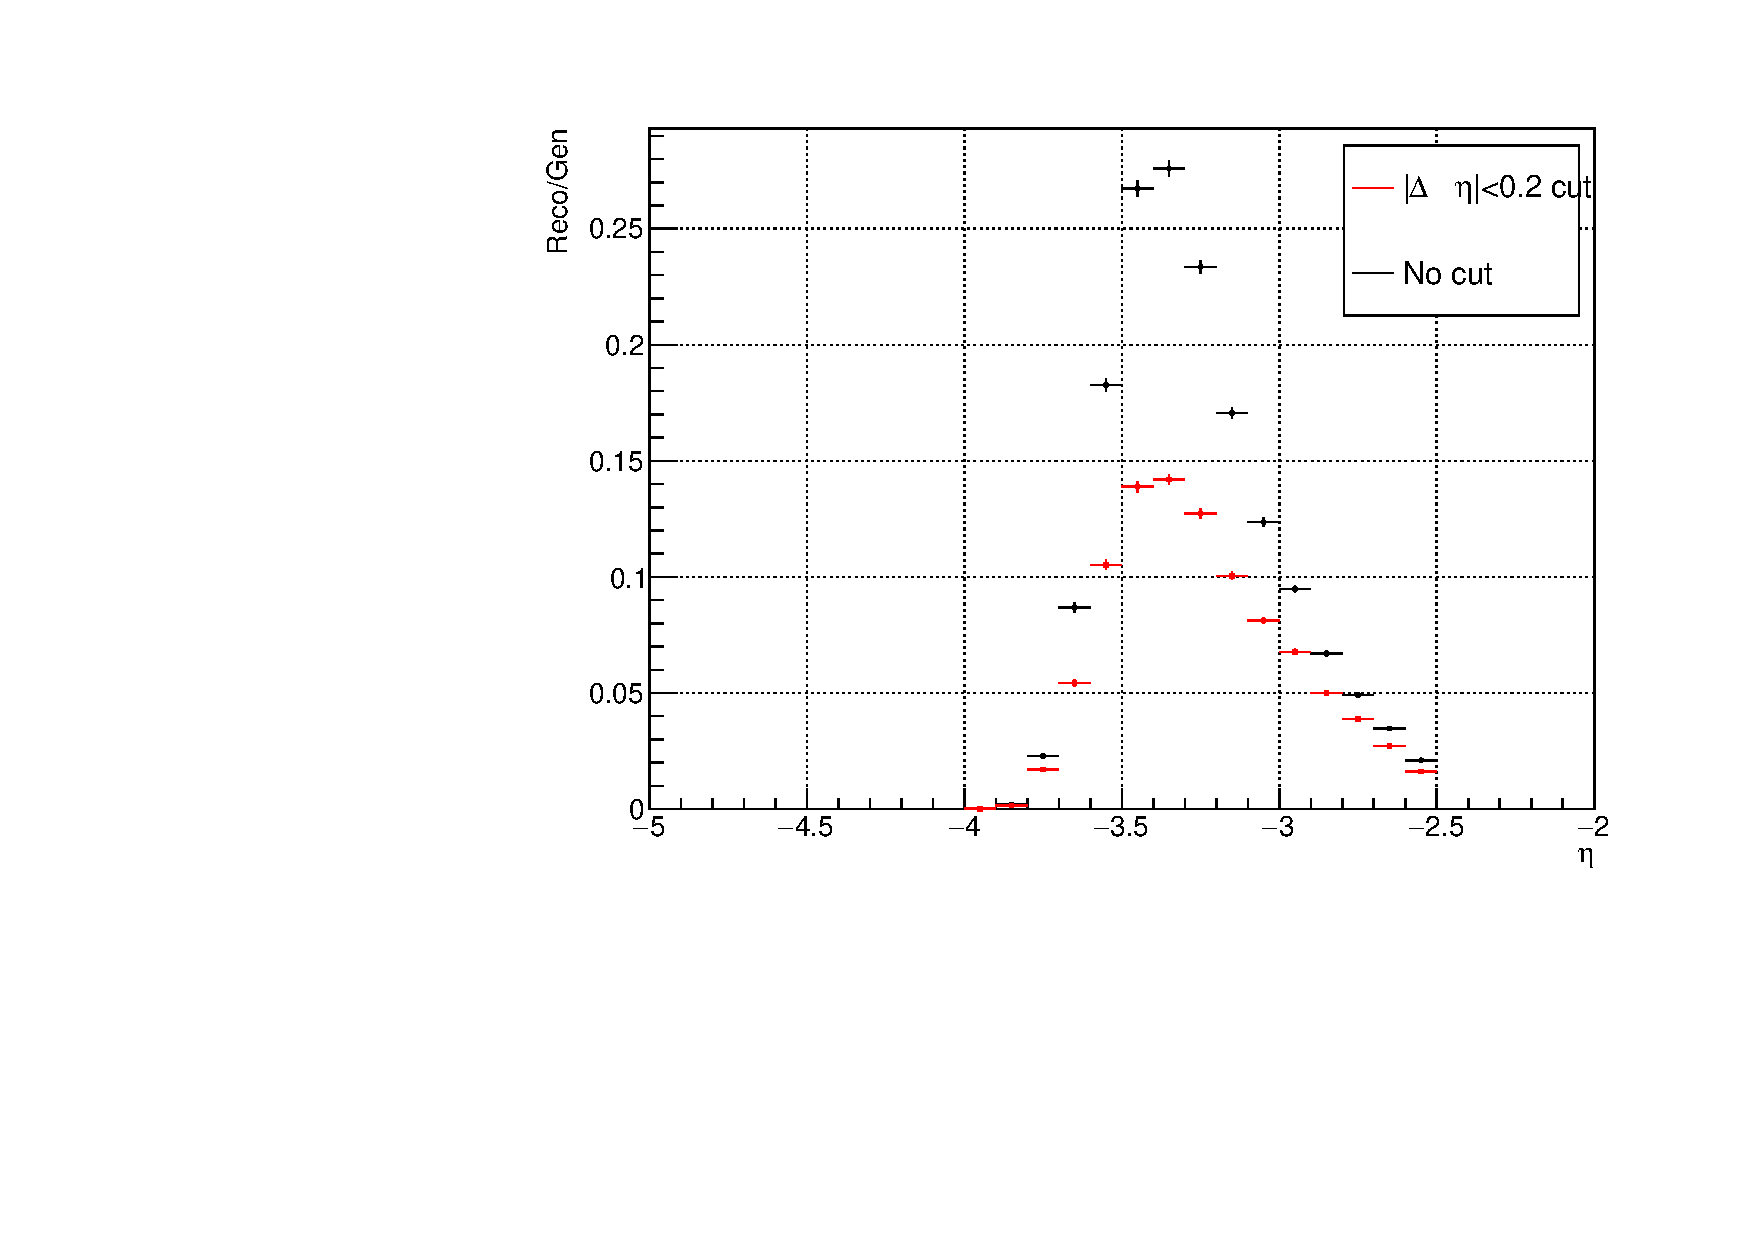
\includegraphics[width=\textwidth]{fig/3_5_6_efficiency_eta.pdf}
                    \captionsetup{labelformat=empty}
                    \caption{Efficency of $\eta$}
                \end{minipage}
                \\
                \vspace{1em}
                \begin{minipage}{0.45\textwidth}
                \centering
                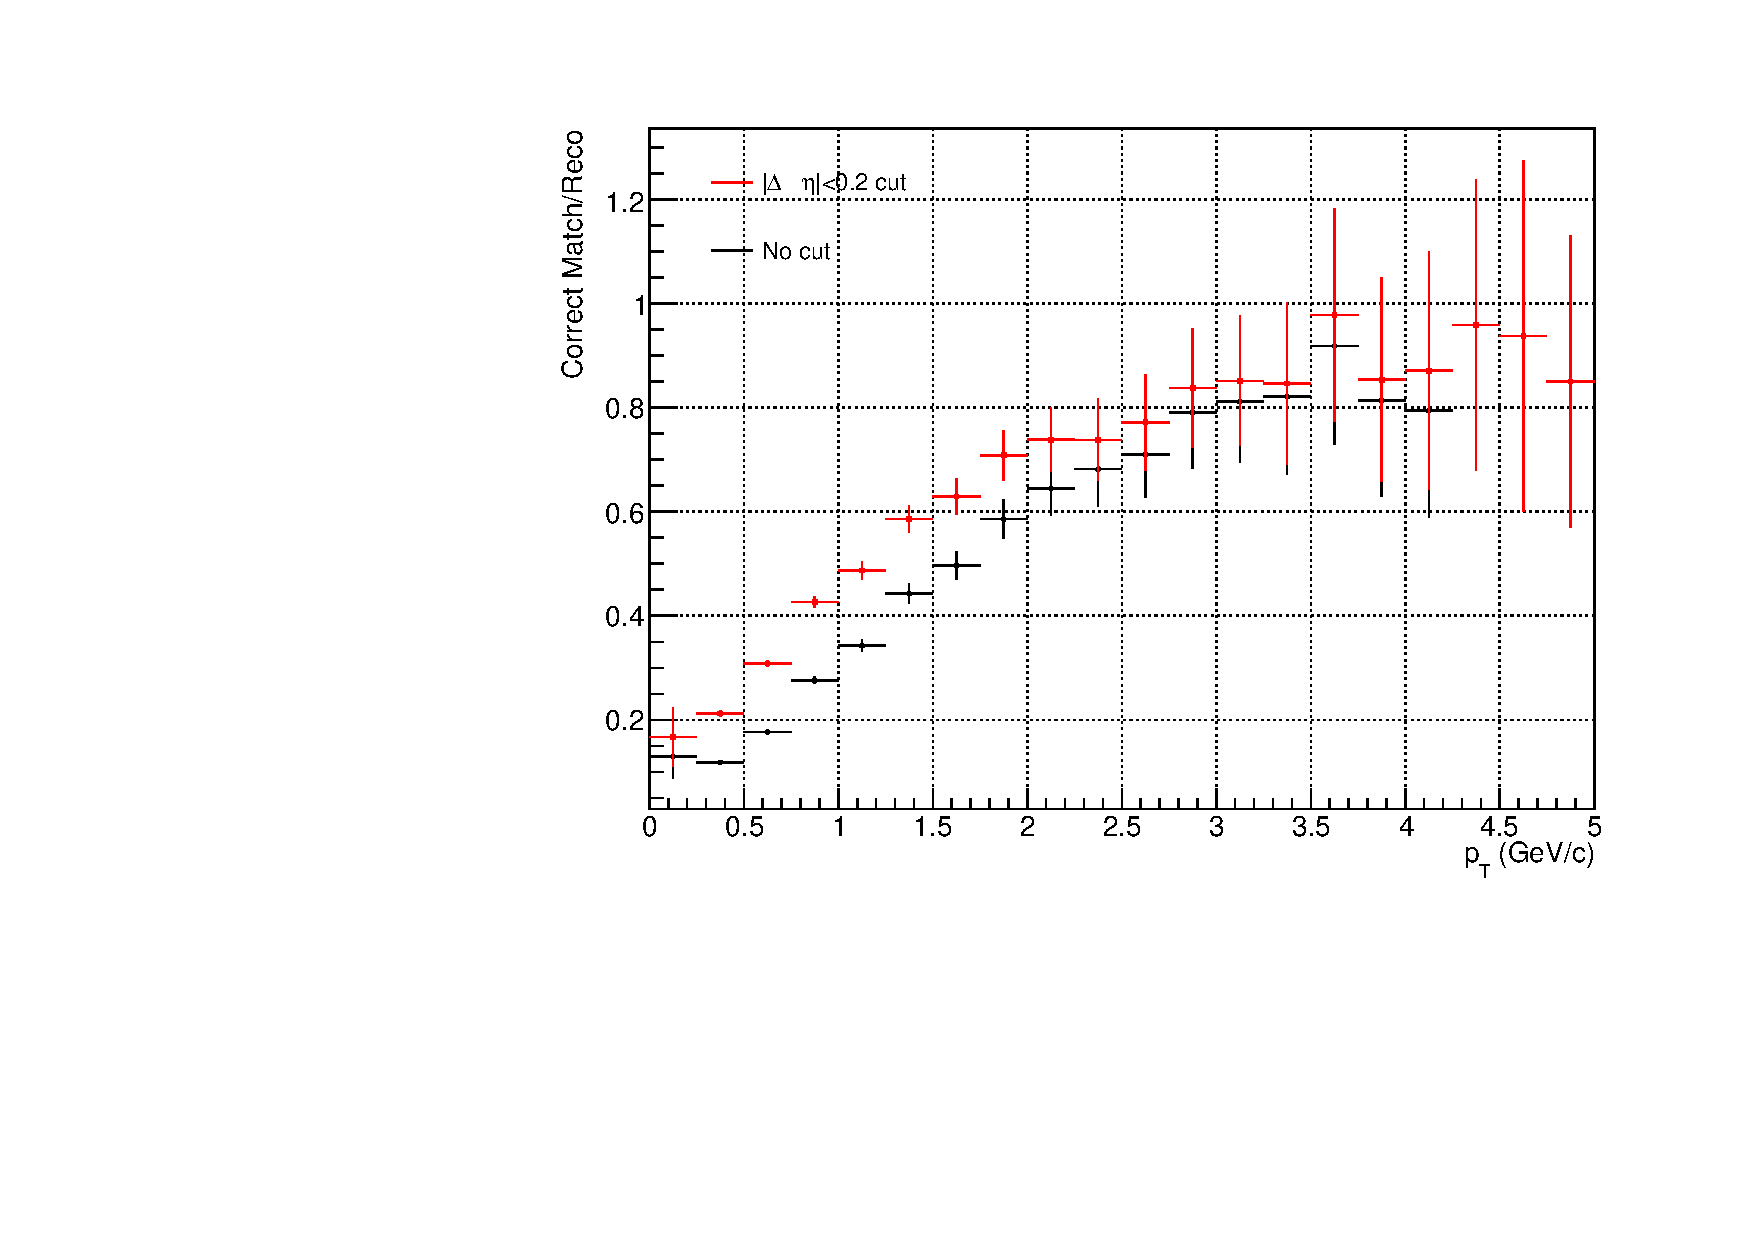
\includegraphics[width=\textwidth]{fig/3_5_6_purity_pt.pdf}
                    \caption{Purity of $p_T$}
                \end{minipage}
                \hfill
                \begin{minipage}{0.45\textwidth}
                    \centering
                    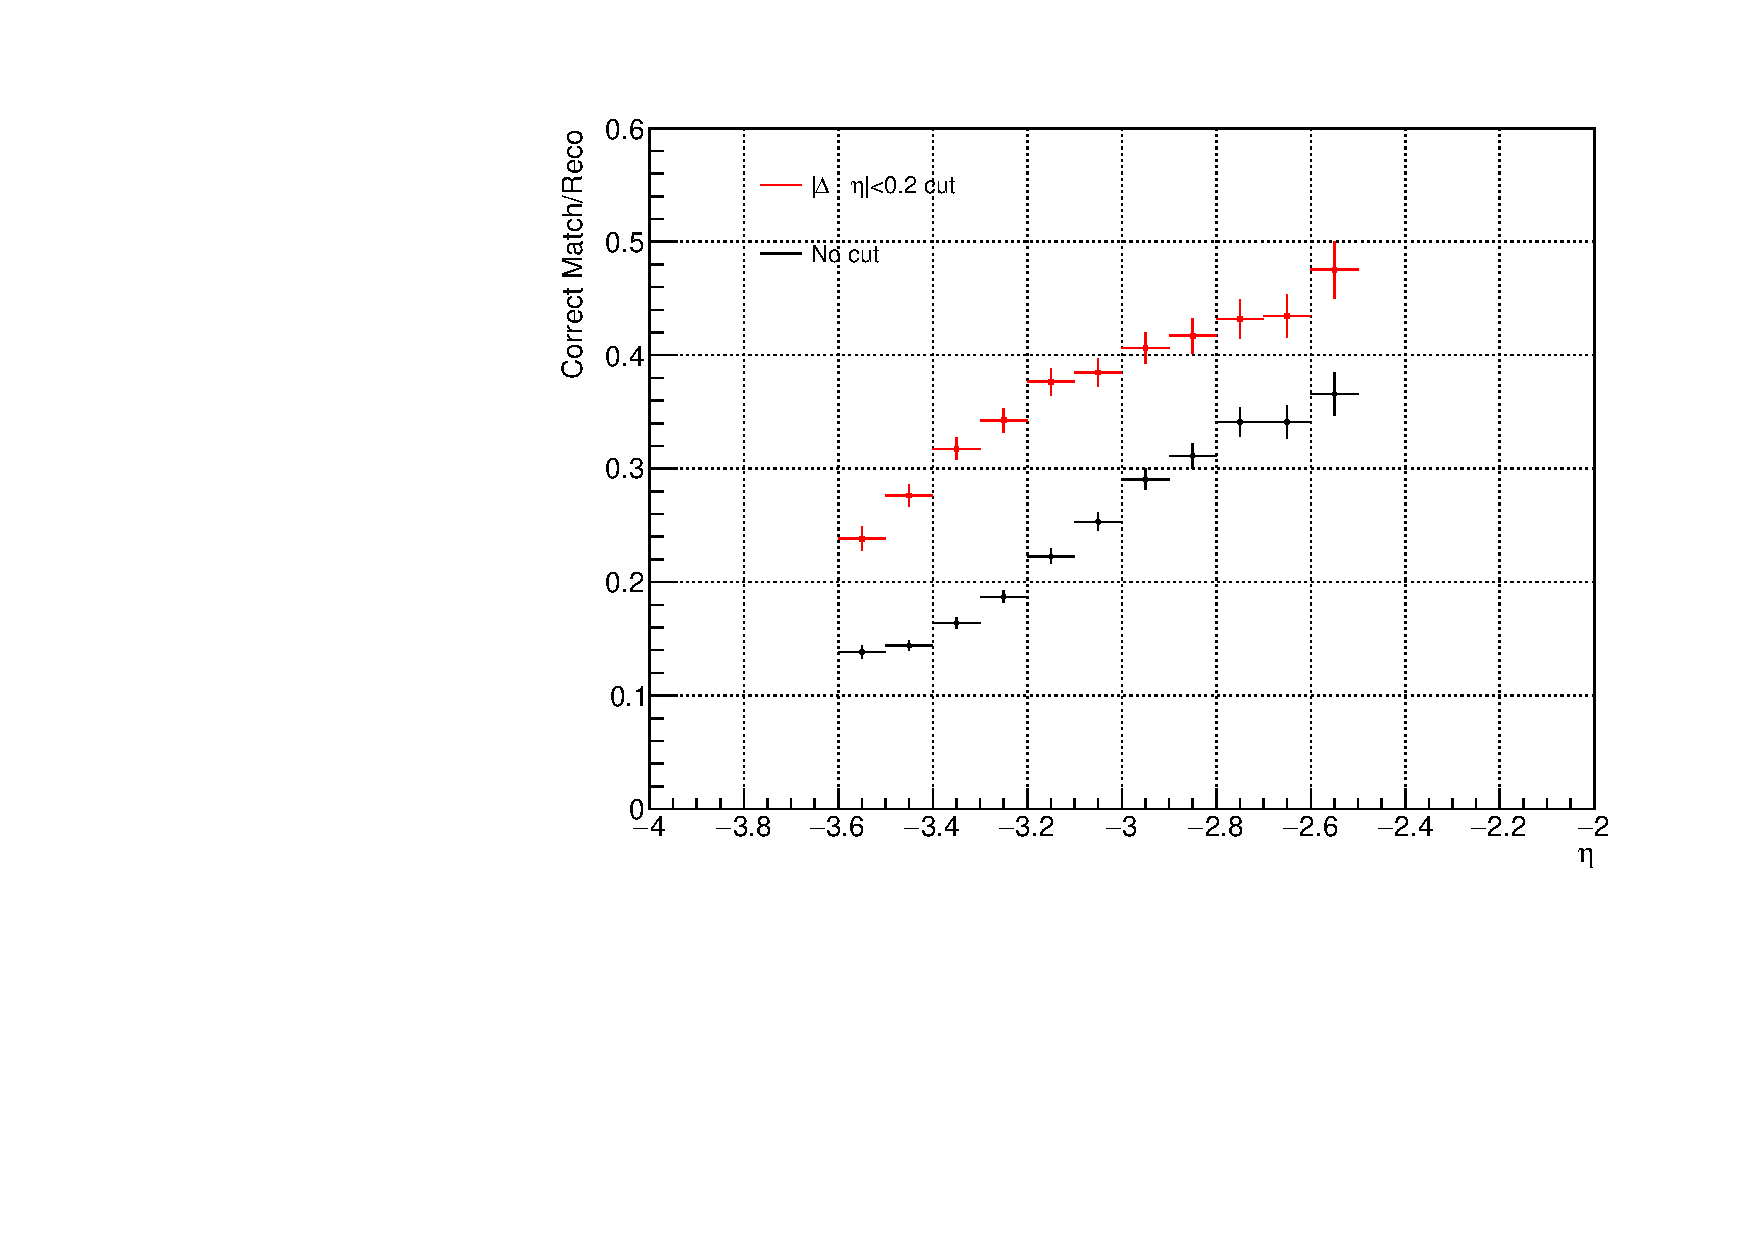
\includegraphics[width=\textwidth]{fig/3_5_6_purity_eta.pdf}
                \caption{Purity of $\eta$} 
                \end{minipage}
                \\
                \vspace{1em}
                \begin{minipage}{0.45\textwidth}
                        \centering
                        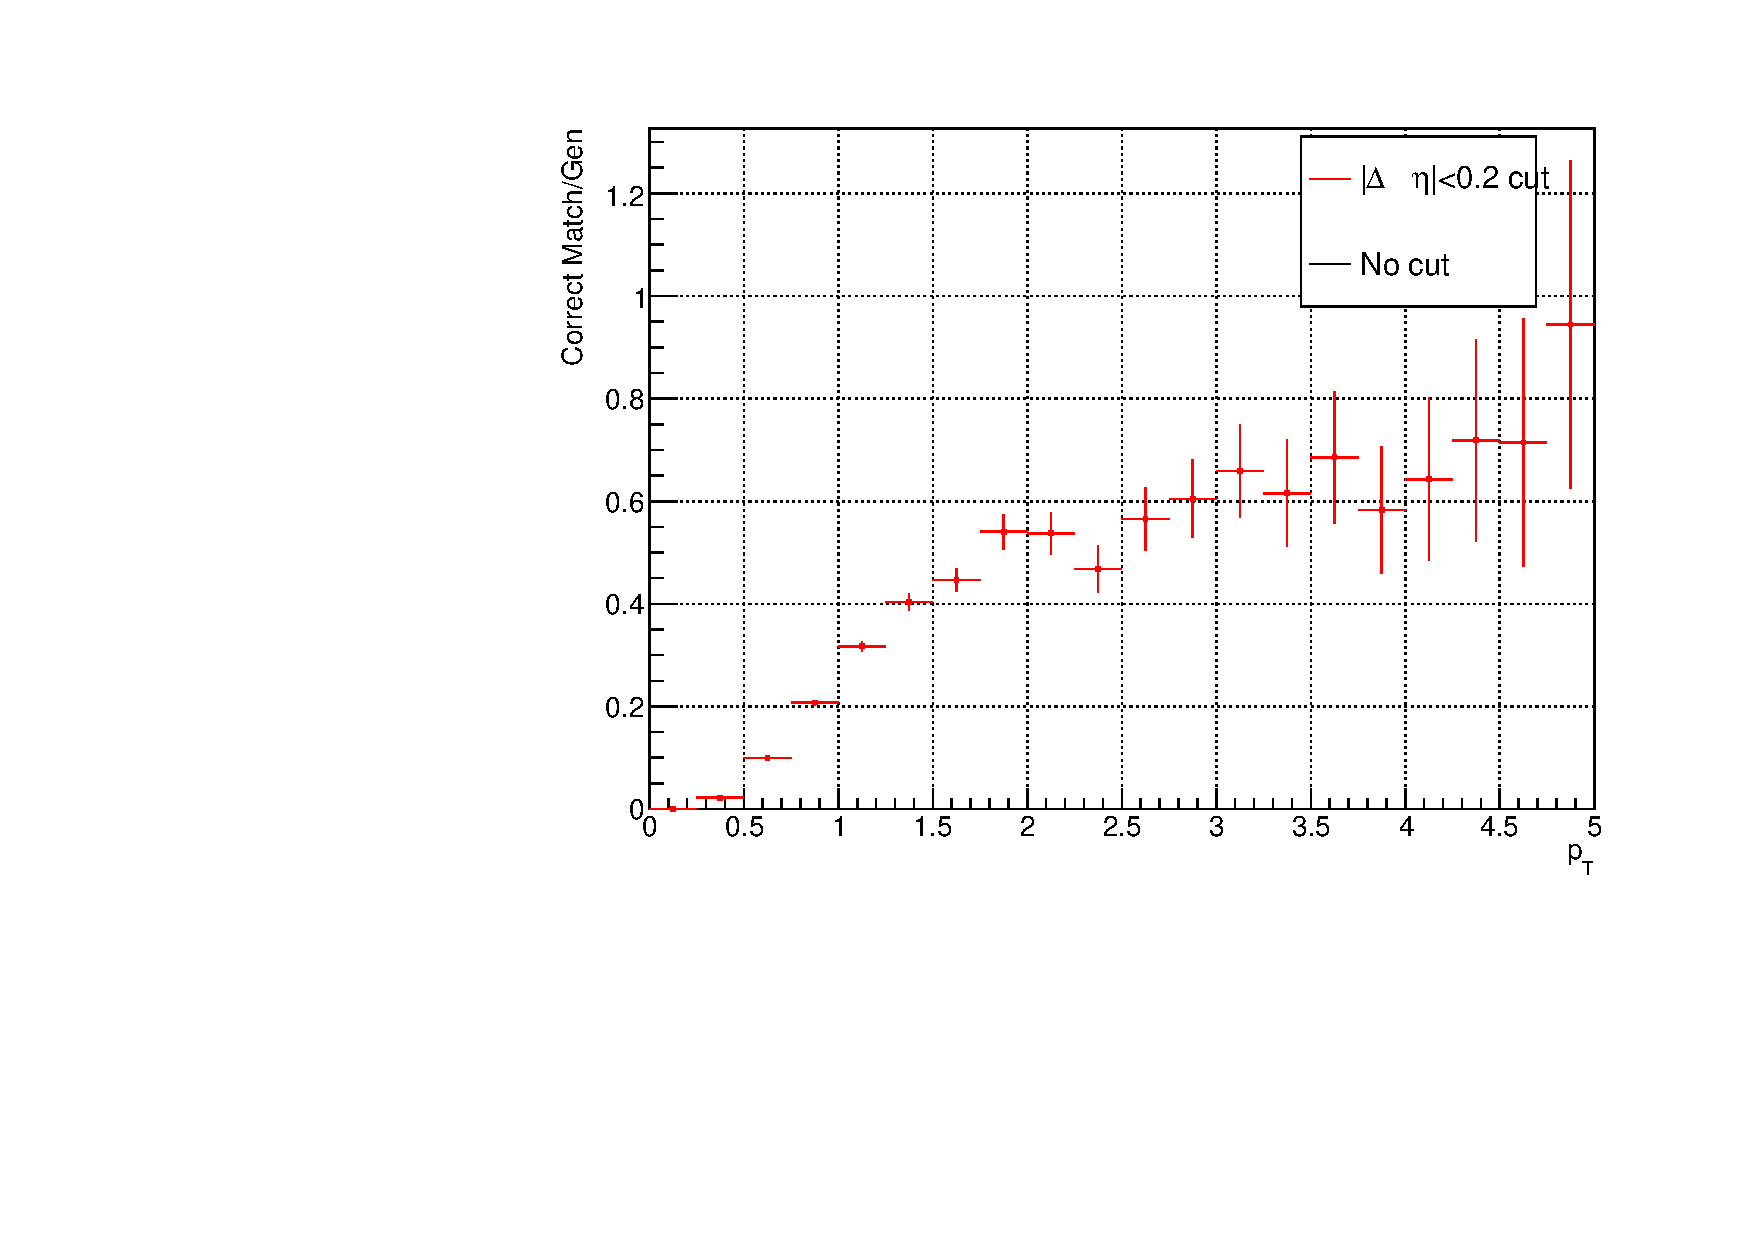
\includegraphics[width=\textwidth]{fig/3_5_6_effpuri_pt.pdf}
                    \caption{Efficency $\times$ Purity of $p_T$}
                \end{minipage}
                \hfill
                \begin{minipage}{0.45\textwidth}
                    \centering
                    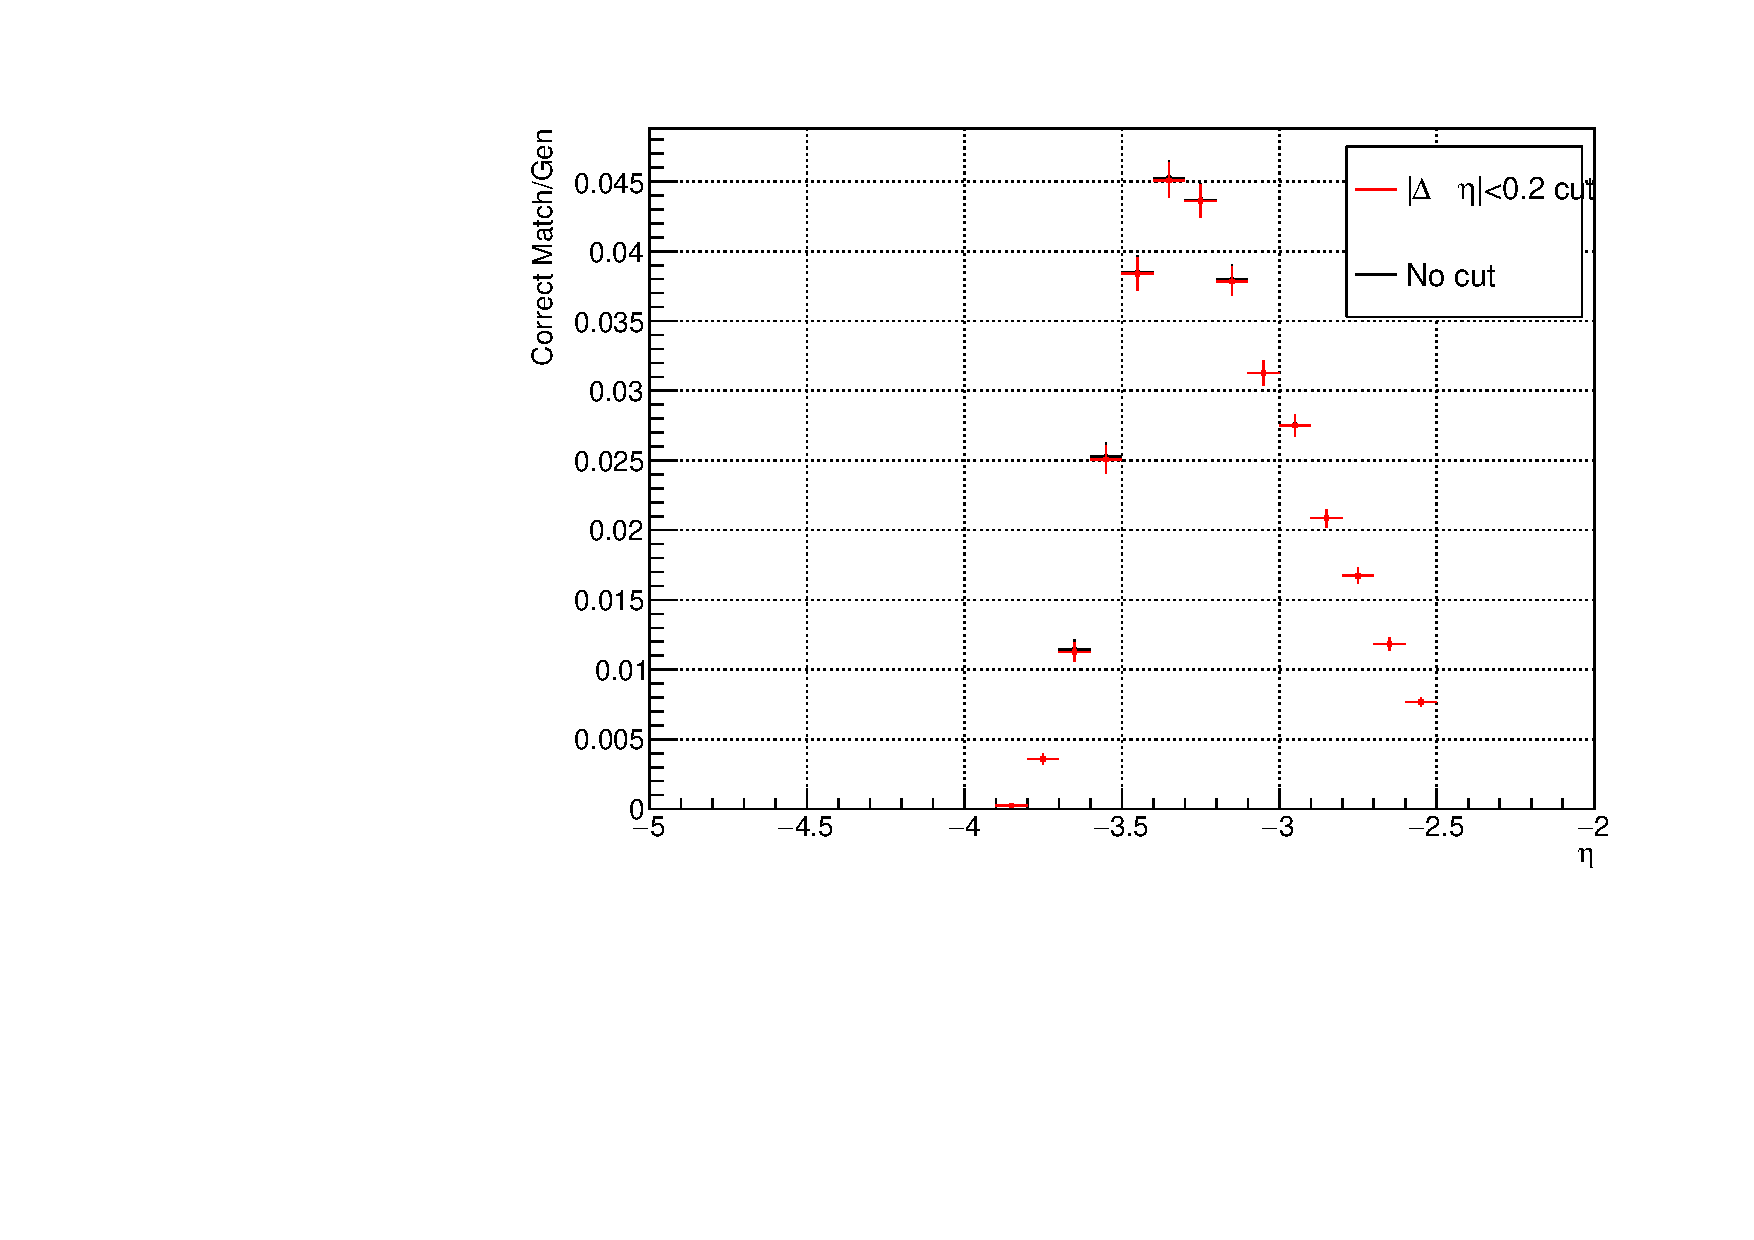
\includegraphics[width=\textwidth]{fig/3_5_6_effpuri_eta.pdf}
                    \caption{Efficency $\times$ Purity of $\eta$}
                \end{minipage}
            \end{figure}
            The \( |\Delta \eta| < 0.2 \) cut was applied in such a way as to discard as few correct match tracks as possible, while removing fake match tracks. For the \( p_T \) distribution, the efficiency drops below 2 GeV, but the matching purity improves. The product of efficiency \(\times\) purity remains unchanged compared to before the cut. This indicates that the cut does not significantly remove correct matches. For the \(\eta\) distribution, efficiency is reduced in the range \( -3.6 < \eta < -3 \), but matching purity improves in the range \( -4 < \eta < -2 \). Similarly, the product of efficiency \(\times\) purity for \(\eta\) also remains unchanged compared to before the cut.